 \documentclass{llncs}

%\documentclass[envcountsame, fleqn]{llncs}
  \usepackage{amsmath, amssymb, latexsym}
  \usepackage{graphicx}
\usepackage{epic,eepic}

%\pagestyle{plain}
\usepackage{listings}
\usepackage{psfrag}
\usepackage{rotating}

\usepackage{url}
\usepackage{amssymb,amsthm, epsfig,amstext}
\usepackage{txfonts}
\usepackage{algorithmic}
\usepackage{algorithm}
\usepackage{graphicx}

\usepackage{mathrsfs}

\usepackage{color, colortbl}

\usepackage{todonotes}
\usepackage{multirow}
\usepackage{float,color}
\usepackage{picinpar,color,xcolor,wrapfig}
\setcounter{secnumdepth}{4}
\sloppy

\pagestyle{plain}

%%%%%%%%%%%%%%%   MACROS  %%%%%%%%%%%%%%%%%%


%!TEX root = popl2018.tex

\newcommand{\set}[1]{\{ #1 \}}
\newcommand{\sequence}[2]{(#1, \ldots, #2)}
\newcommand{\couple}[2]{(#1,#2)}
\newcommand{\pair}[2]{(#1,#2)}
\newcommand{\triple}[3]{(#1,#2,#3)}
\newcommand{\quadruple}[4]{(#1,#2,#3,#4)}
\newcommand{\tuple}[2]{(#1,\ldots,#2)}
\newcommand{\Nat}{\ensuremath{\mathbb{N}}}
\newcommand{\Rat}{\ensuremath{\mathbb{Q}}}
\newcommand{\Rea}{\ensuremath{\mathbb{R}}}
\newcommand{\Zed}{\ensuremath{\mathbb{Z}}}
%\newcommand{\true}{\top}
%\newcommand{\false}{\perp}
\newcommand{\bottom}{\perp}
%% \newcommand{\powerset}[1]{{\cal P}(#1)}
\newcommand{\npowerset}[2]{{\cal P}^{#1}(#2)}
\newcommand{\finitepowerset}[1]{{\cal P}_f(#1)}
\newcommand{\level}[2]{L_{#1}(#2)}
\newcommand{\card}[1]{\mbox{card}(#1)}
\newcommand{\range}[1]{\mathtt{ran}(#1)}
\newcommand{\astring}{s}

\newcommand{\Cc}{\mathcal{C}}


\newcommand {\notof}{\ensuremath{\neg}}
\newcommand {\myand}{\ensuremath{\wedge}}
\newcommand {\myor}{\ensuremath{\vee}}
\newcommand {\mynext}{\mbox{{\sf X}}}
\newcommand {\until}{\mbox{{\sf U}}}
\newcommand {\sometimes}{\mbox{{\sf F}}}
\newcommand {\previous}{\mynext^{-1}}
\newcommand {\since}{\mbox{{\sf S}}}
\newcommand {\fminusone}{\mbox{{\sf F}}^{-1}}
\newcommand {\everywhere}[1]{\mbox{{\sf Everywhere}}(#1)}



\newcommand{\aatomic}{{\rm A}}
\newcommand{\aset}{X}
\newcommand{\asetbis}{Y}
\newcommand{\asetter}{Z}

\newcommand{\avarprop}{p}
\newcommand{\avarpropbis}{q}
\newcommand{\avarpropter}{r}
\newcommand{\varprop}{{\rm PROP}} % Set of atomic propositions (for a given logic)

% formulae

\newcommand{\aformula}{\astateformula} % a formula
\newcommand{\aformulabis}{\astateformulabis} % another formula (when at least 2 are present)
\newcommand{\aformulater}{\astateformulater} % another formula (when at least 3 are present)
\newcommand{\asetformulae}{X}
\newcommand{\subf}[1]{sub(#1)}

\newcommand{\aautomaton}{{\mathbb A}}
\newcommand{\aautomatonbis}{{\mathbb B}}

\newcommand {\length}[1] {\ensuremath{|#1|}}



% Equivalences
\newcommand{\egdef}{\stackrel{\mbox{\begin{tiny}def\end{tiny}}}{=}} % =def=
\newcommand{\eqdef}{\stackrel{\mbox{\begin{tiny}def\end{tiny}}}{=}} % =def=
\newcommand{\equivdef}{\stackrel{\mbox{\begin{tiny}def\end{tiny}}}{\equivaut}} % <=def=>
\newcommand{\equivaut}{\;\Leftrightarrow\;}

\newcommand{\ainfword}{\sigma}

\newcommand{\amap}{\mathfrak{f}}
\newcommand{\amapbis}{\mathfrak{g}}

\newcommand{\step}[1]{\xrightarrow{\!\!#1\!\!}}
\newcommand{\backstep}[1]{\xleftarrow{\!\!#1\!\!}}

\newcommand {\aedge}[1] {\ensuremath{\stackrel{#1}{\longrightarrow}}}
\newcommand {\aedgeprime}[1] {\ensuremath{\stackrel{#1}{\longrightarrow'}}}
\newcommand {\afrac}[1] {\ensuremath{\mathit{frac}(#1)}}
\newcommand {\cl}[1] {\ensuremath{\mathit{cl}(#1)}}
\newcommand {\sfc}[1] {\ensuremath{\mathit{sfc}(#1)}}
\newcommand {\dunion} {\ensuremath{\uplus}}
\newcommand {\edge} {\ensuremath{\longrightarrow}}
\newcommand {\emptyword}{\ensuremath{\epsilon}}
\newcommand {\floor}[1] {\ensuremath{\lfloor #1 \rfloor}}
\newcommand {\intersection} {\ensuremath{\cap}}
\newcommand {\union} {\ensuremath{\cup}}
\newcommand {\vals}[2] {\ensuremath{\mathit{val}_{#2}(#1)}}



\newcommand {\pspace} {\textsc{pspace}}
\newcommand {\nlogspace} {\textsc{nlogspace}}
\newcommand {\logspace} {\textsc{logspace}}
\newcommand {\expspace} {\textsc{expspace}}
\newcommand {\np} {\textsc{np}}
\newcommand {\threeexptime} {\textsc{3exptime}}
\newcommand {\polytime} {\textsc{p}}
\newcommand{\twoexpspace}{\textsc{2expspace}}
\newcommand{\threeexpspace}{\textsc{3expspace}}
\newcommand {\nexptime} {\textsc{nexptime}}



\newcommand{\aalphabet}{\Sigma}     % an alphabet, A is already used for atoms
\newcommand{\aword}{\mathfrak{u}}
\newcommand{\awordbis}{\mathfrak{v}}



\newcommand{\aassertion}{P}
\newcommand{\aassertionbis}{Q}
\newcommand{\aexpression}{e}
\newcommand{\aexpressionbis}{f}
\newcommand{\avariable}{\mathtt{x}}
\newcommand{\uniquevar}{\mathtt{u}}
\newcommand{\uniquevarbis}{\mathtt{v}}
\newcommand{\avariablebis}{\mathtt{y}}
\newcommand{\avariableter}{\mathtt{z}}
\newcommand{\nullconstant}{\mathtt{null}}
\newcommand{\nilvalue}{nil}
\newcommand{\emptyconstant}{\mathtt{emp}}
\newcommand{\infheap}{\mathtt{inf}}
\newcommand{\saturated}{\mathtt{Saturated}}

\newcommand{\astateformula}{\phi}
\newcommand{\astateformulabis}{\psi}
\newcommand{\astateformulater}{\varphi}
%%
\newcommand{\separate}{\ast}
\newcommand{\sep}{\separate}
\newcommand{\size}{\mathtt{size}}
\newcommand{\sizeeq}[1]{\mathtt{size} \ = \ #1}
\newcommand{\alloc}[1]{\mathtt{alloc}(#1)}
\newcommand{\allocb}[2]{\mathtt{alloc}^{-1}[#2](#1)}
\newcommand{\isol}[1]{\mathtt{isoloc}(#1)}
\newcommand{\icell}{\mathtt{isocell}}
\newcommand{\malloc}{\mathtt{malloc}}
\newcommand{\cons}{\mathtt{cons}}
\newcommand{\new}{\mathtt{new}}
\newcommand{\free}[1]{\mathtt{free} \ #1}
\newcommand{\maxform}[1]{\mathtt{maxForms}(#1)}
\newcommand{\locations}[1]{\mathtt{loc}(#1)}
\newcommand{\values}{\mathtt{Val}}
\newcommand{\aheap}{\mathfrak{h}}
\newcommand{\avaluation}{\mathfrak{V}}
\newcommand{\heaps}{\mathcal{H}}
\newcommand{\astore}{\mathfrak{s}}
\newcommand{\stores}{\mathcal{S}}
\newcommand{\amodel}{\mathfrak{M}}
\newcommand{\alabel}{\ell}

\newcommand{\aprogram}{\mathtt{PROG}}
\newcommand{\programs}{\mathtt{P}}
\newcommand{\ctprograms}{\programs^{ct}}
\newcommand{\aninstruction}{\mathtt{instr}}
\newcommand{\ainstruction}{\mathtt{instr}}
\newcommand{\instructions}{\mathtt{I}}
\newcommand{\aguard}{\ensuremath{g}}
\newcommand{\guards}{\ensuremath{G}}
\newcommand{\domain}[1]{\mathtt{dom}(#1)}
\newcommand{\memory}{\stores\times\heaps}
\newcommand{\skipinstruction}{\mathtt{skip}}

\newcommand{\execution}{\mathtt{comp}}
\newcommand{\aux}{\mathtt{embd}}
\newcommand{\runof}{run}
\newcommand{\anexecution}{e}


\newcommand{\aletter}{\ensuremath{a}}
\newcommand{\aletterbis}{\ensuremath{b}}
\newcommand{\alocation}{\mathfrak{l}}

\newcommand{\pointsl}[1]{\stackrel{#1}{\hookrightarrow}}
\newcommand{\ppointsl}[1]{\stackrel{#1}{\mapsto}}
\newcommand{\ourhook}[1]{\stackrel{#1}{\hookrightarrow}}
\newcommand{\ltrue}{{\sf true}}
\newcommand{\lfalse}{{\sf false}}


\newcommand{\variables}{\mathtt{FVAR}}
\newcommand{\pvariables}{\mathtt{PVAR}}
\newcommand{\secvariables}{\mathtt{SVAR}}
\newcommand{\logique}[1]{\mathtt{FO}(#1)}



\newcommand{\atranslation}{\mathfrak{t}}
\newcommand{\nbpred}[1]{\widetilde{\sharp #1}}
\newcommand{\nbpredstar}[1]{\widetilde{\sharp #1}^{\star}}
\newcommand{\isolated}{\mathtt{isol}}
\newcommand{\stdmarks}{\mathtt{envir}}
\newcommand{\relation}[1]{\mathtt{relation}_{#1}}
\newcommand{\freevar}{\mathtt{FV}}
\newcommand{\notonmark}{\mathtt{notonenv}}
\newcommand{\InVal}[1]{\mathtt{InVal}\!\left(#1\right)}
\newcommand{\NotOnEnv}[1]{\mathtt{NotOnEnv}\!\left(#1\right)}
\newcommand{\PartOfVal}[1]{\mathtt{PartOfVal}\!\left(#1\right)}
%\newcommand{\nbpreds}[3]{\sharp #1 \geq #2}
\newcommand{\defstyle}[1]{{\emph{#1}}}

\newcommand{\cut}[1]{}
\newcommand{\interval}[2]{[#1,#2]}
\newcommand{\buniquevar}{\overline{\uniquevar}}
\newcommand{\bbuniquevar}{\overline{\overline{\uniquevar}}}
\newcommand{\magicwand}{\mathop{\mbox{$\mbox{$-~$}\!\!\!\!\ast$}}}
\newcommand{\wand}{\magicwand}
\newcommand{\septraction}{\stackrel{\hsize0pt \vbox to0pt{\vss\hbox to0pt{\hss\raisebox{-6pt}{\footnotesize$\lnot$}\hss}\vss}}{\magicwand}}
%% \newcommand{\reach}{\mathtt{reach}}
\mathchardef\mhyphen="2D % hyphen while in math mode

\newcommand{\adataword}{\mathfrak{dw}}
\newcommand{\adatum}{\mathfrak{d}}

\newcommand{\collectionknives}{\mathtt{ks}}
\newcommand{\collectionknivesfork}[1]{\mathtt{ksfs}_{=#1}}
\newcommand{\collectionknivesforks}{\mathtt{ksfs}}
\newcommand{\collectionkniveslargeforks}{\mathtt{kslfs}}


\newcommand{\acounter}{\mathtt{C}}

\newcommand{\fotwo}[3]{{\mbox{FO2}_{#1,#2}(#3)}}
\newcommand{\mtrans}[1]{t\!\left(#1\right)^{\Box}}
\newcommand{\mbtrans}[2]{\mtrans{#2}_{#1}}


\newcommand{\alogic}{\mathfrak{L}}


\newcommand{\semantics}[1]{\ensuremath{[ #1 ]}}


\newcommand{\adomino}{\mathfrak{d}}
\newcommand{\atile}{\mathfrak{d}}
\newcommand{\atiling}{\mathfrak{t}}

\newcommand{\hori}{\mathtt{h}}
\newcommand{\verti}{\mathtt{v}}
\newcommand{\domi}{\mathtt{d}}

\newcommand{\cpyrel}{\mathfrak{cp}}

\newcommand{\cntcmp}{\mathfrak{C}}

\newcommand{\heapdag}{\mathfrak{G}}

\newcommand{\onmainpath}{\mathtt{mp}}

\newcommand{\tree}{\mathtt{tree}}

%\newcommand{\tile}{\mathtt{tile}}

\newcommand{\type}{\mathtt{type}}

\newcommand{\ptype}{\mathtt{ptype}}

\newcommand{\exttype}{\mathtt{exttype}}

\newcommand{\anctypes}{\mathtt{AncTypes}}

\newcommand{\destypes}{\mathtt{DesTypes}}

\newcommand{\inctypes}{\mathtt{IncTypes}}

\newcommand{\treeic}{\mathtt{treeIC}}

\newcommand{\trs}{\mathfrak{trs}}


\newcommand{\nin}{\not \in}
\newcommand{\cupplus}{\uplus}
\newcommand{\aunarypred}{\mathtt{P}}


\newcommand{\hide}[1]{}

\newcommand{\eval}[2]{\llbracket#1\rrbracket_{#2}}
\newcommand\cur{\mathsf{cur}}
\newcommand\dom{\mathsf{dom}}
\newcommand\rng{\mathsf{rng}}

\newcommand\dd{\mathbb{D}}
\newcommand\nat{\mathbb{N}}


\newcommand\cA{\mathcal{A}}
\newcommand\cB{\mathcal{B}}
\newcommand\cC{\mathcal{C}}
\newcommand\cE{\mathcal{E}}
\newcommand\cG{\mathcal{G}}
\newcommand\Ll{\mathcal{L}}
\newcommand\cM{\mathcal{M}}
\newcommand\cP{\mathcal{P}}
\newcommand\cR{\mathcal{R}}
\newcommand\cS{\mathcal{S}}
\newcommand\cT{\mathcal{T}}

\newcommand\vard{\mathfrak{d}}

\newcommand\replaceall{\mathsf{replaceAll}}
\newcommand\indexof{\mathsf{IndexOf}}


\newcommand\strline{\mathsf{SL}}

\newcommand\pstrline{\mathsf{SL_{pure}}}

\newcommand\search{\mathsf{search}}

\newcommand\verify{\mathsf{verify}}

\newcommand\searchleft{\mathsf{searchLeft}}

\newcommand\searchlong{\mathsf{searchLong}}


\newcommand\pref{\mathsf{Pref}}

\newcommand\wprof{\mathsf{WP}}

\newcommand\vars{\mathsf{Vars}}

\newcommand\dep{\mathsf{Dep}}
\newcommand\ptn{\mathsf{Ptn}}

\newcommand\src{\mathsf{src}}
\newcommand\strtorep{\mathsf{strToRep}}

\newcommand\rpleft{\mathsf{l}}
\newcommand\rpright{\mathsf{r}}


\newcommand\srcnd{\mathsf{srcND}}

\newcommand\ctxt{\mathsf{ctxt}}


\newcommand\ctxts{\mathsf{Ctxts}}

\newcommand\sprt{\mathsf{sprt}}

\newcommand\val{\mathsf{val}}

\newcommand\srclen{\mathsf{srcLen}}

\newcommand\rpleftlen{\mathsf{lLen}}


\newcommand\dfs{\mathsf{DFS}}

\newcommand\repr{\mathsf{rep}}

\newcommand\red{\mathsf{red}}

\newcommand\gfun{\mathcal{F}}


\newcommand{\leftmost}{{\sf leftmost}}
\newcommand{\longest}{{\sf longest}}

\newcommand{\arbidx}{{\sf Idx_{arb}}}
\newcommand{\dmdidx}{{\sf Idx_{dmd}}}
\newcommand{\lftlen}{{\sf Len_{lft}}}

%\newtheorem{remark}[theorem]{Remark}


%%%%%%%%%%%%%%%%%%%%%%%%%%%%%%%%%%%%%%%%%%%%

\newcommand{\zhilin}[1]{\color{cyan} {ZL: #1 :LZ} \color{black}}
\newcommand{\tl}[1]{\color{purple} {TL: #1 :LT} \color{black}}
\newcommand{\anthony}[1]{\color{blue} {AL: #1 :LA} \color{black}}
\newcommand{\matt}[1]{\color{blue} {MH: #1 :HM} \color{black}}
\newcommand{\philipp}[1]{\color{blue} {PR: #1 :RP} \color{black}}

%%%%%%%%%%%%%%%%%%%%%%%%%%%%%%%%%%%%%%%%%%%%


\title{A Decision Procedure for Path Feasibility of \\
String Numeric Programs}


\author{}

\institute{ }

\begin{document}


%Regular Papers should not exceed 20 pages in LNCS format, not counting references and appendices.
%
%Regular papers at CAV 2020 will follow a full double blind review process, which means that author names and affiliations must be omitted from the submission. Additionally, if a submission refers to prior work done by the authors, the reference should be made in the third person. These are firm submission requirements, and any regular paper that does not conform to these requirements will be rejected without review.
%
%Authors can include a clearly marked appendix at the end of their submissions that is exempt from the page limit restrictions. However, the reviewers are not obliged to read the contents of these appendices. These papers should contain original research and sufficient detail to assess the merits and relevance of the contribution. Papers will be evaluated on basis of a combination of correctness, technical depth, significance, novelty, clarity, and elegance.

\maketitle

\begin{abstract}
String and numeric constraints are widely used in programs, especially in Web programs, e.g. Javascript and PHP. 
In this paper, we consider a string logic which can express both string and numeric constraints, in particular, the logic includes not only pure string operations, e.g. concatenation, replaceAll, reverse, and transducers, but also those operations involving the integer data type, e.g. length, substring, and indexOf functions.  
We propose a decision procedure for the logic, based on a variant of cost register automata (Alur et al. LICS 2013), which seamlessly extends that of the OSTRICH solver. Moreover, we implement the decision procedure on top of OSTRICH. The experimental results show that the decision procedure performances very well on a wide range of benchmarks. 
\end{abstract}

%\section{Introduction}
%\label{intro}
%
%\section{Preliminaries}
%\label{prel}
%
%Definition for NFA, NFT.

%%%%%%%%%%%%%%%%%%%%%%%%%%%%%%%%%%%%%%%%%%%%%%%%%%%%%%%
\section{Introduction}

20 pages, excluding references.

%!TEX root = popl2018.tex

\section{Introduction}

The problem of %satisfiability of logical theories over strings
automatically solving string constraints (aka satisfiability of logical theories over
strings) has recently witnessed
renewed interest %in the programming language and verification community
\cite{Berkeley-JavaScript,TCJ16,LB16,YABI14,S3,Abdulla14,Abdulla17,DV13,symbolic-transducer,BEK} 
because of important applications in the analysis of 
string-manipulating programs. For example,
program analysis techniques like symbolic execution \cite{king76,DART,EXE} 
would
%. For example, program analysis techniques like
%symbolic execution \cite{king76} (or variants like dynamic symbolic execution
%\cite{DART,EXE}) will 
systematically explore executions in a program and collect symbolic path 
constraints, which could then be solved using a constraint solver and
used to determine which location in the program to continue exploring.
To successfully apply a constraint solver in this instance, it is
crucial that the constraint language precisely model the data types in the
program, along with the data-type operations used. In the context of
string-manipulating programs, this could include 
concatenation, regular constraints (i.e. pattern matching against a regular
expression), string-length functions, and the string-replace functions, among 
many others.

%For scripting
%languages (e.g. Python, PHP, and JavaScript), which have grown in popularity
%in recent years, numerous string 
%There are several well-established research threads on this satisfiability 
%problem depending on 
%which string operations are permitted in the theory. 
Perhaps the most well-known theory of strings for applications to analysing
string-manipulating programs is the theory of strings with concatenation 
(aka \emph{word equations}),
whose decidability status was settled positively by Makanin \cite{Makanin}
in 1977 after it was open for many years. More importantly, 
this theory remains 
decidable even when regular constraints are incorporated into the 
language \cite{Schulz}. However, whether adding the string-length function
results preserves the decidability remains a long-standing open problem
\cite{Vijay-length,buchi}.

%\OMIT{
%which is crucial for 
Another important string operation (especially, in popular scripting
languages like Python, JavaScript, and PHP) is the string-replace function, 
which may be used to replace either the first occurrence or
all occurrences of a string (a string constant/variable, or a regular expression) by 
another string (a string constant/variable). The replace function (especially 
the replace-all functionality) is omnipresent in HTML5 applications
\cite{LB16,TCJ16,YABI14}. 
%\mat{What does it mean for the replace function to be convincingly argued?}
For example, a standard industry defense against cross-site scripting 
(XSS) vulnerabilities includes sanitising untrusted strings before adding them
into the DOM (Document Object Model) or the HTML document. 
This is typically done by %replacing every occurrence of
various metacharacter-escaping mechanisms (e.g. see 
\cite{Kern14,BEK,OWASP-XSS}), e.g., backslash-escape, which replaces \emph{every
occurrence} of quotes and double-quotes (i.e. \verb+'+ and \verb+"+) in the
string by \verb+\'+ and \verb+\"+. 
In addition
to sanitisers, common JavaScript functionalities like \texttt{document.write()} 
and \texttt{innerHTML} apply an \emph{implicit browser transduction} --- which
decodes HTML codes (e.g. \verb+&#39;+ is replaced by \verb+'+) in the input 
string --- before inserting the input string into the DOM.
Both of these examples can be expressed by (perhaps multiple) 
applications of the string-replace function.
Moreover, although these examples replace constants by constants, the popularity of template systems such as Mustache~\cite{Mustache} demonstrate the need for replacements involving variables.
Using Mustache, a web-developer, for example, may define an HTML fragment with placeholders that is instantiated with user data during the construction of the delivered page.
\mat{Need to say more what template systems are?}
\anthony{Better mention closure templates I think, Matt. They do both
mustache-kind of replace plus sanitisers. They call these strict autoescaping
templates. See \cite{SSS11}.}

%Concatenation: 8\%
%Replace-all: 8\%

In general, the string-replace function has three parameters, and in the current mainstream language such as Python and JavaScript, all of the three parameters can be inserted as string variables. As result, when we perform program analysis for, for instance, detecting security vulnerabilities as described as above, one often obtains string constraints of the form $z= \replaceall(x, p, y)$, where $x,y$ are string constants/variables, and $p$ is either a string constant/variable, or a regular expression.
Such a constraint means that $z$ is obtained by replacing all occurrences of $p$ in $x$ by $y$. For convenience, we call $x, p, y$ as the subject, the pattern, and the replacement parameters respectively. 

%for instance $z=\replaceall(x,"aa", y)$, meaning that $z$ is obtained by replacing all occurrences of $aa$ in $x$ by $y$. Solving string constraints involving this type of constraints is crucial, but unfortunately, is not supported by the current technique. There are two reasons:

%The string-replace function is formalised as $\replaceall(x, p, y)$, where $x,y$ are string constants/variables, and $p$ is either a string constant/variable, or a regular expression. The semantics of $\replaceall(x, p, y)$ is to replace all occurrences of $p$ in $x$ with $y$. For convenience, we call $x, p, y$ as the subject, the pattern, and the replacement parameters respectively. 

%The string-replace function is a quite powerful string operation. To see this, let us consider the constraint $C \equiv z = \replaceall(x, 0, y) \wedge x \in (01)^* \wedge y \in 0^*$. Then the set of values of $z$ that make $C$ satisfied is $\{(0^n 1)^* \mid n \in \Nat \}$.


The $\replaceall$ function is a powerful string operation that goes beyond the 
expressiveness of concatenation. 
Recently, it was shown in \cite{LB16} that any theory of strings containing the 
string-replace function (even the most restricted version where 
pattern/replacement strings are both constant strings) becomes undecidable if 
we do not impose some kind of
straight-line (aka acyclicity) restriction on the formulas. 
\OMIT{
As a matter of fact, it was shown in~\cite{LB16} that any 
incorporating a simple form of the $\replaceall$ function, where the pattern and the replacement are both string constants, into the theory of concatenations already results in an undecidable theory of strings.  
%that lies beyond 
%the expressiveness of the theory of concatenation, 
Therefore, it is challenging to reason about the string-replace function in its general form. 
}
%In~\cite{LB16}, a theory of strings involving concatenation and finite state transducers was considered. The $\replaceall$ function where the pattern is a string constant or regular expression, the third parameter is a constant can be seen as a special case of finite state transducers. It was shown therein that incorporating the simple form of the $\replaceall$ function into the theory of concatenations already results in an undecidable theory of strings. 
A partial result 
%can be deduced from the results 
from the following recent POPL paper in~\cite{LB16} provides decidability
for the straight-line fragment of the theory of strings involving 
concatenation, regular constraints, and the $\replaceall$ function where the 
pattern and the replacement are both string constants. 
The decision procedure therein was obtained for finite-state transducers, which
subsume the aforementioned simple form of the $\replaceall$ function, but
\emph{not} in its most form.
The straight-line restriction is natural in the sense that it reflects the shape of formulas typically generated by symbolic execution.  Nevertheless, the decidability boundary of the straight-line fragment of string constraints involving the $\replaceall$ function in this general form, e.g. when the replacement parameter is a variable, remains an open question which we address in this article.
\mat{Am i right to say we tackle it here?}

%% If you're looking for all the omitted and hidden semi-paragraphs that were here, checkout version 407adea8bf0c0564f064f43ae3b355fc8ac901d7. -- Matt

\paragraph{Example}

We give a simple example demonstrating a (naive) XSS vulnerability to illustrate the use of string-replace functions.
Consider the HTML fragment below.
\begin{minted}{html}
    <h1>User 
        <span onMouseOver="popupText('{{bio}}')">
            {{userName}} </span> </h1>
\end{minted}
This HTML fragment is a template as might be used with systems such as Mustache to display a user on a webpage.
For each user that is to be displayed -- with their username and biography stored in variables \emph{name} and \emph{biography} respectively -- the string \verb+{{userName}}+ will be replaced by \emph{name} and the string \verb+{{bio}}+ will be replaced by \emph{bio}.
For example, a user \verb+Amelia+ with biography \verb+Amelia was born in 1979...+ would result in the HTML below.
\begin{minted}{html}
    <h1>User 
        <span onMouseOver="popupText('Amelia was born in 1979...')">
            Amelia </span> </h1>
\end{minted}
This HTML would display \verb+User Amelia+, and, when the mouse is placed over \verb+Amelia+, her biography would appear, thanks to the \verb+onMouseOver+ attribute in the \verb+span+ element.

Unfortunately, this template could be insecure if the user biography is not adequately sanitised: 
A user could enter a malicious biography, such as \verb+'); alert('Boo!'); alert('+ which would cause the following instantiation of the \verb+span+ element\footnote{
    Readers familiar with Mustache may expect single quotes to be automatically escaped.
    However, this was not part of the specification until 2014, before which, support was inconsistent, which may have caught some developers off-guard~\cite{MustacheSingleQuote}.    
}.
\begin{minted}{html}
    <span onMouseOver="popupText(''); alert('Boo!'); alert('')">
\end{minted}
Now, when the mouse is placed over the user name, the malicious JavaScript \verb+alert('Boo!')+ is executed.

The presence of such malicious injections of code can be detected using string constraint solving and XSS \emph{attack patterns} $P$, which are given as regular expressions~\cite{BCFJKKV08,SAHMMS10,YABI14}.
For our example, given an attack pattern $P$ and template $t$, we would generate the constraint
\[
    x_1 = \replaceall(t, \verb+{{userName}}+, \mathit{user})
    \land
    x_2 = \replaceall(x_1, \verb+{{bio}}+, \mathit{bio})
    \land
    x_2 \in P
\]
which would detect if the HTML generated by instantiating the template is susceptible to the attack identified by $P$.
\mat{ANTHONY: can you verify/expand on my use of attack patterns?  I just copied it wholesale and blindly from your POPL 2016.}

\paragraph{Contribution.} We investigate the decidability boundary of the theory of strings involving concatenation, regular constraints, and the $\replaceall$ function, with the straight-line constraint introduced in \cite{LB16}. 

We first show that with the $\replaceall$ function in its general form, the concatenation operation is in fact \emph{redundant}, in the sense that it can be simulated by the $\replaceall$ function. This motivates us to consider a theory of strings where the $\replaceall$ function, instead of the concatenation operation, and the regular constraints, are the basic modalities. We focus on the straight-line fragment of this theory, denoted by $\strline[\replaceall]$.

We obtain the following results for the satisfiability problem of $\strline[\replaceall]$.
\begin{itemize}
\item If the pattern parameters of the $\replaceall$ function are allowed to be variables, then the satisfiability of $\strline[\replaceall]$ is undecidable (cf. Proposition~\ref{prop-und-pat-var}).
%
\item If the pattern parameters of the $\replaceall$ function are regular expressions, then the satisfiability of $\strline[\replaceall]$ is decidable and in EXPSPACE (cf. Theorem~\ref{thm-main}). In addition, we show that the satisfiability problem is PSPACE-complete for several cases that are meaningful in practice (cf. Corollary~\ref{cor-pspace}).
%
\item If $\strline[\replaceall]$, where the pattern parameters of the $\replaceall$ function are regular expressions, is extended with any of integer constraints, character constraints, or constraints involving the $\indexof$ function, then the satisfiability becomes undecidable again (cf. Theorem~\ref{thm-ext-int} and  Proposition~\ref{prop-ext-char}-\ref{prop-indexof}).
\end{itemize}

Our decision procedure for $\strline[\replaceall]$ where the pattern parameters of the $\replaceall$ function are regular expressions follows the automata-theoretical approach. The key idea is explained as follows: Let us consider the simple formula $C \equiv x = \replaceall(y, a, z) \wedge x \in e_1 \wedge y \in e_2 \wedge z \in e_3$. 
Suppose that $\cA_1,\cA_2,\cA_3$ are the nondeterministic finite state automata corresponding to $e_1,e_2,e_3$ respectively. 
We effectively eliminate the use of $\replaceall$ by nondeterministically generating from $\cA_1$ a new regular constraint $\cA'_2$ for $y$ -- and $\cA'_3$ for $z$ respectively -- that incorporates the effect of the $\replaceall$. Then the satisfiability of $C$ is turned into testing the nonemptiness of the intersection of $\cA_2$ and $\cA'_2$, as well as the nonemptiness of the intersection of $\cA_3$ and $\cA'_3$. When there are multiple occurrences of the $\replaceall$ function, this process can be iterated. 
Our decision procedure enjoys the following advantages:
\begin{itemize}
	\item it is automata-theoretic and built on a neat automata construction, moreover, when the formula is satisfiable, a solution can be synthesised, 
	
	\item the decision procedure is modular and amenable to implementation,  in the sense that the $\replaceall$ terms are removed one by one to generate more and more regular constraints,
	
	\item the decision procedure requires exponential space, but for the cases that are meaningful in practice, the decision procedure uses only polynomial space. 
\end{itemize}

%EXPSPACE algorithm
%
%a table to summarise the results.


\paragraph{Organisation.} 
This paper is organised as follows: Preliminaries are given in Section~\ref{sec-prel}. The core string language is defined in Section~\ref{sec-core}. The main results of this paper are summarised in Section~\ref{sec-sat}. The decision procedure is presented in Section~\ref{sec:replaceallsl}-\ref{sec:replaceallre}, case by case. The extensions of the core string language are investigated in Section~\ref{sec-ext}. The related work can be found in Section~\ref{sec-rel}.


%%%%%%%%%%%%%%%%%%%%%%%%%%%%%%%%%%%%%%%%%%%%%%%%%%%%%%%
\section{Preliminaries}\label{sec:prel}

%!TEX root = popl2018.tex

\section{Preliminaries}\label{sec-prel}

\paragraph{General notation} 
Let $\mathbb{Z}$ and $\Nat$ denote the set of integers and natural numbers respectively. For $k \in \Nat$, let $[k] = \{1,\cdots, k\}$. For a vector $\vec{x}=(x_1,\cdots, x_n)$, let $|\vec{x}|$ denote the length of $\vec{x}$ (i.e., $n$) and  $\vec{x}[i]$ denote $x_i$ for each $i \in [n]$. %, . For a vector $\vec{x} = (x_1, \cdots, x_n)$, let 
%$\red(\vec{x})$ denote the \emph{reduction} of $\vec{x}$, more specifically, the vector $(x_{i_1},\cdots, x_{i_m})$ such that for each $j \in [m]$, $x_{i_j}$ is different from all $x_1, \cdots, x_{i_j-1}$. For instance, $\red(a,a,b,b,c)=(a,b,c)$.
%\tl{red is for reduced?}


\paragraph{Regular languages}
Fix a finite \emph{alphabet} $\Sigma$. Elements in $\Sigma^*$ are called \emph{strings}. Let $\varepsilon$ denote the empty string and  $\Sigma^+ = \Sigma^* \setminus \{\varepsilon\}$. We will use $a,b,\cdots$ to denote letters from $\Sigma$ and $u, v, w, \cdots$ to denote strings from $\Sigma^*$. For a string $u \in \Sigma^*$, let $|u|$ denote the \emph{length} of $u$ (in particular, $|\varepsilon|=0$). A \emph{position} of a nonempty string $u$ of length $n$ is a number $i \in [n]$ (Note that the first position is $1$, instead of  0). In addition, for $i \in [|u|]$, let $u[i]$ denote the $i$-th letter of $u$. 
For two strings $u_1, u_2$, we use $u_1 \cdot u_2$ to denote the \emph{concatenation} of $u_1$ and $u_2$, that is, the string $v$ such that $|v|= |u_1| + |u_2|$ and for each $i \in [|u_1|]$, $v[i]= u_1[i]$ and for each $i \in |u_2|$, $v[|u_1|+i]=u_2[i]$. Let $u, v$ be two strings. If $v = u \cdot v'$ for some string $v'$, then $u$ is said to be a \emph{prefix} of $v$. In addition, if $u \neq v$, then $u$ is said to be a \emph{strict} prefix of $v$. If $u$ is a prefix of $v$, that is, $v = u \cdot v'$ for some string $v'$, then 
we use $u^{-1} v$ to denote $v'$. In particular, $\varepsilon^{-1} v = v$.

A \emph{language} over $\Sigma$ is a subset of $\Sigma^*$. We will use $L_1, L_2, \dots$ to denote languages. For two languages $L_1, L_2$, we use $L_1 \cup L_2$ to denote the union of $L_1$ and $L_2$, and $L_1 \cdot L_2$ to denote the concatenation of $L_1$ and $L_2$, that is, the language $\{u_1 \cdot u_2 \mid u_1 \in L_1, u_2 \in L_2\}$. For a language $L$ and $n \in \Nat$, we define $L^n$, the \emph{iteration} of $L$ for $n$ times, inductively as follows: $L^0=\{\varepsilon\}$ and $L^{n} =L \cdot L^{n-1}$ for $n > 0$. We also use $L^*$ to denote the iteration of $L$ for arbitrarily many times, that is, $L^* = \bigcup \limits_{n \in \Nat} L^n$. Moreover, let $L^+ = \bigcup \limits_{n \in \Nat \setminus \{0\}} L^n$.

\begin{definition}[Regular expressions $\regexp$]
	\[e \eqdef \emptyset \mid \varepsilon \mid a \mid e + e \mid e \concat e \mid e^*, \mbox{ where } a \in \Sigma. \]
	Since $+$ is associative and commutative, we also write $(e_1 + e_2) + e_3$ as $e_1 + e_2 + e_3$ for brevity. We use the abbreviation $e^+ \equiv e \concat e^*$. Moreover, for $\Gamma = \{a_1, \cdots, a_n\}\subseteq \Sigma$, we use the abbreviations $\Gamma \equiv a_1 + \cdots + a_n$ and $\Gamma^\ast \equiv (a_1 + \cdots + a_n)^\ast$. 
\end{definition}
We define $\Ll(e)$ to be the language defined by $e$, that is, the set of strings that match $e$, inductively as follows: $\Ll(\emptyset) =\emptyset$,
%\begin{itemize}
%\item 
$\Ll(\varepsilon) =\{\varepsilon\}$,
%
%\item 
$\Ll(a)= \{a\}$,
%
%\item 
$\Ll(e_1 + e_2) = \Ll(e_1) \cup \Ll(e_2)$,
%
%\item 
$\Ll(e_1 \concat e_2) = \Ll(e_1) \cdot \Ll(e_2)$,
%
%\item 
$\Ll(e_1^*)=(\Ll(e_1))^*$.
%\end{itemize}
In addition, we use $|e|$ to denote the number of symbols occurring in $e$.

A \emph{nondeterministic finite automaton} (NFA) $\cA$ on $\Sigma$ is a tuple $(Q, \delta, q_0, F)$, where $Q$ is a finite set of \emph{states}, $q_0 \in Q$ is the \emph{initial} state, $F \subseteq Q$ is the set of \emph{final} states, and $\delta \subseteq Q \times \Sigma \times Q$ is the \emph{transition relation}. For a string $w = a_1 \dots a_n$, a \emph{run} of $\cA$ on $w$ is a state sequence $q_0 \dots q_n$ such that for each $i \in [n]$, $(q_{i-1}, a_i, q_i) \in \delta$. A run $q_0 \dots q_n$ is \emph{accepting} if $q_n \in F$. A string $w$ is \emph{accepted} by $\cA$ if there is an accepting run of $\cA$ on $w$. We use $\Ll(\cA)$ to denote the language defined by $\cA$, that is, the set of strings accepted by $\cA$. We will use $\cA, \cB, \cdots$ to denote NFAs. 
%An NFA $\cA$ is \emph{deterministic} if for each $(q, \sigma) \in Q \times \Sigma$, there is at most one $q' \in Q$ such that $(q, a, q') \in \delta$. An NFA $\cA$ is \emph{complete} if for each $(q, \sigma) \in Q \times \Sigma$, there is at least one $q' \in Q$ such that $(q, a, q') \in \delta$. We assume that all NFA considered in this paper are complete.  An NFA $\cA$ is \emph{unambiguous} if for each word $w$, there is \emph{at most one accepting} run of $\cA$ on $w$.
For a string $w= a_1 \dots a_n$, we also use the notation $q_1 \xrightarrow[\cA]{w} q_{n+1}$ to denote the fact that there are $q_2,\dots, q_n \in Q$ such that for each $i \in [n]$, $(q_i, a_i, q_{i+1}) \in \delta$.  For an NFA $\cA=(Q, \delta, q_0, F)$ and $q, q' \in Q$, we use $\cA(q,q')$ to denote the NFA obtained from $\cA$ by changing the initial state to $q$ and the set of final states to $\{q'\}$. The \emph{size} of an NFA $\cA=(Q, \delta, q_0, F)$, denoted by $|\cA|$, is defined as $|Q|$, the number of states. For convenience, we will also call an NFA without initial and final states, that is, a pair $(Q, \delta)$, as a \emph{transition graph}. 


\begin{proposition}[\cite{HU79}]
The following facts hold for regular expressions and NFAs.
\begin{itemize}
\item Regular expressions and NFAs are expressively equivalent. In particular, from a regular expression, an equivalent NFA can be constructed in linear time.  
%
\item NFAs are closed under all Boolean operations, namely, union, intersection, and complementation.
\end{itemize}
\end{proposition}

In particular, given two NFA $\cA_1=(Q_1, \delta_1, q_{0,1}, F_1)$ and $\cA_2=(Q_2, \delta_2, q_{0,2}, F_2)$ on $\Sigma$, to define the intersection of $\Ll(\cA_1)$ and $\Ll(\cA_2)$, the \emph{product automaton} of $\cA_1$ and $\cA_2$, denoted by $\cA_1 \times \cA_2$, is constructed as the NFA $(Q_1 \times Q_2, \delta, (q_{0,1}, q_{0,2}), F_1 \times F_2)$, where $\delta$ comprises the transitions $((q_1, q_2), a, (q'_1, q'_2))$ such that $(q_1, a, q'_1) \in \delta_1$ and $(q_2, a, q'_2) \in \delta_2$.  

\paragraph{Graph-theoretical notation}
The term DAG stands for \emph{directed acyclic graphs}, which are finite directed graphs $(V, E)$ with no directed cycles. That is, each DAG consists of finitely many vertices and edges, with each edge directed from one vertex to another, such that there is no way to start at any vertex $\mathit{v}$ and follow a consistently-directed sequence of edges that eventually loops back to $\mathit{v}$ again. Equivalently, a DAG is a directed graph that has a topological ordering, which is a sequence of the vertices such that every edge is directed from earlier to later in the sequence. Let $G=(V,E)$ be a DAG. An edge from $\mathit{v}$ to $\mathit{v'}$ in $G$ is called an \emph{incoming} edge of $\mathit{v'}$ and an \emph{outgoing} edge of $\mathit{v}$. If there is an edge from $\mathit{v}$ to $\mathit{v'}$ in $G$, then $\mathit{v'}$ is called a \emph{successor} of $\mathit{v}$ and $\mathit{v}$ is called a \emph{predecessor} of $\mathit{v'}$. A \emph{path} in $G$ is a sequence $\mathit{v}_0 \mathit{e}_1 \mathit{v}_1 \cdots \mathit{v}_{n-1} \mathit{e}_n \mathit{v}_n$ such that for each $i \in [n]$, $e_i$ is an edge from $\mathit{v}_{i-1}$ to $\mathit{v}_i$. The \emph{length} of a path $\mathit{v}_0 e_1 \mathit{v}_1 \cdots \mathit{v}_{n-1} e_n \mathit{v}_n$ in $G$ is $n$, i.e. the number of edges in the path. If there is a path from $\mathit{v}$ to $\mathit{v'}$ (resp. from $\mathit{v'}$ to $\mathit{v}$) in $G$, then $\mathit{v'}$ is said to be \emph{reachable} (resp. \emph{co-reachable}) from $\mathit{v}$ in $G$. If $\mathit{v}$ is reachable from $\mathit{v'}$ in $G$, then $\mathit{v'}$ is also called an \emph{ancestor} of $\mathit{v}$ in $G$. In addition, an edge from $\mathit{v'}$ to $\mathit{v''}$ is said to be reachable (resp. co-reachable) from $\mathit{v}$ if $\mathit{v'}$ is reachable from $\mathit{v}$ (resp. $\mathit{v''}$ is co-reachable from $\mathit{v}$). The \emph{in-degree} (resp. \emph{out-degree}) of a vertex $\mathit{v}$ is the number of incoming (resp. outgoing) edges of $\mathit{v}$. 
%A vertex $\mathit{v}$ in $G$ is said to be a \emph{join} vertex if the in-degree of $\mathit{v}$ is at least two. 
%A DAG $G$ is called an \emph{arborescence} if there is a vertex $v_0$ such that all the vertices are reachable from $v_0$ in $G$, in addition, there are no join vertices in $G$.  
A \emph{subgraph} $G'$ of $G=(V,E)$ is a pair $(V', E')$ such that $V' \subseteq V$ and $E' \subseteq V' \times V'$. Let $G'$ be a subgraph of $G$. Then $G \setminus G'$ is the graph obtained from $G$ by removing all the edges in $G'$. 


%%%%%%%%%%%%%%%%%%%%%%diamond removed for simplicity%%%%%%%%%%%%%%%%%%%%%%%%%%
%%%%%%%%%%%%%%%%%%%%%%diamond removed for simplicity%%%%%%%%%%%%%%%%%%%%%%%%%%
\hide{
\begin{definition}[Diamond and diamond graph]
Let $G=(V,E)$  be a DAG and $v,v' \in V$ with $v \neq v'$. Then a diamond in $G$ from $v$ to $v'$ is a pair of paths $\pi_1, \pi_2$ from $v$ to $v'$ such that  $\pi_1$ and $\pi_2$ are vertex-disjoint, except $v$ and $v'$. The diamond graph of $G$, denoted by $\cG_{\sf dmd}(G)$, is the graph $(G, E \cup E')$, where $E'$ comprises the pairs $(v,v')$ such that $v\neq v'$ and there is a diamond from $v$ to $v'$. The edges in $E'$ are called the diamond edges of $\cG_{\sf dmd}(G)$.
\end{definition}


\begin{definition}[Diamond index]
Let $G=(V,E)$ be a DAG and $\cG_{\sf dmd}(G)$ be the diamond graph of $G$. Then the diamond index of $G$, denoted by $\dmdidx(G)$, is the maximum number of diamond edges in a path of $\cG_{\sf dmd}(G)$.
\end{definition}

\begin{example}
Example for diamond index
\end{example}

\begin{proposition}\label{prop-num-path}
Let $G=(V,E)$ be a DAG such that the out-degree of each vertex is at most two. Then there are $n^{O(\dmdidx(G))}$ different paths\footnote{two paths are different iff the set of edges in the two paths are different.}  in $G$.
\end{proposition}
}
%%%%%%%%%%%%%%%%%%%%%%diamond removed for simplicity%%%%%%%%%%%%%%%%%%%%%%%%%%
%%%%%%%%%%%%%%%%%%%%%%diamond removed for simplicity%%%%%%%%%%%%%%%%%%%%%%%%%%

% copy from Lin's paper. 

\paragraph{Computational complexity}
In this paper, we study not only decidability but also the complexity of string logics. 
%Pinpointing the
%precise complexity of verification problems is not only of fundamental
%importance, 
%\mat{Do we want to stress this?  We have gaps!}
%but also it often suggests algorithmic techniques
%that are most suitable for attacking the problem in practice.
In this paper, we deal with the following computational complexity
classes (see \cite{HU79} for more details): 
%P (problems solvable in polynomial-time), 
PSPACE (problems solvable in polynomial
space and thus in exponential time), and EXPSPACE (problems solvable
in exponential space and thus in double exponential time). Verification
problems that have complexity PSPACE or beyond (see \cite{BK08}
for a few examples) have substantially benefited from techniques
like symbolic model checking \cite{McMillan}. 
%As we shall see later, our complexity
%upper bound also suggests the maximum lengths of words
%that need to be explored to guarantee completeness.

%=====================================================================================================
%=====================================================================================================

\section{The core constraint language}\label{sec-core}

In this section, we define a general string constraint language that supports word equations, the concatenation, the $\replaceall$ function, and regular constraints.  Throughout this section, we fix an alphabet $\Sigma$.



\subsection{Semantics of the $\replaceall$ function}
To define the semantics of the $\replaceall$ function, we note that the function encompasses three parameters: the first parameter is the \emph{subject} string, the second parameter is a \emph{pattern} that is a string or a regular expression, and the third parameter is the \emph{replacement} string. When the pattern parameter is a string, the semantics is somehow self-explanatory. However, when it is a regular expression, there is no consensus on the semantics even for the mainstream programming languages such as Python and Javascript.
 %where replaceall functions are extensively used. 
 This is particularly the case when interpreting the union (aka alternation) operator in regular expressions or performing a $\replaceall$ with a pattern that matches $\varepsilon$. In this paper, we mainly 
 focus on the semantics of \emph{leftmost and longest matching}.
Our handling of $\varepsilon$ matches is consistent with our testing of the implementation in Python and the \texttt{sed} command with the \texttt{--posix} flag.
We also assume union is commutative (e.g.\ $\replaceall(aa, a + aa, b) = \replaceall(aa, aa + a, b) = b$) as specified by POSIX, but often ignored in practice (where $bb$ is a common result in the former case).

%%%%%%%%%%%%%%%%%%%%%%%%%%%%%%%%%%%%%%%%%
\hide{
\begin{definition}
Let $u, v$ be two strings such that $v = v_1 u v_2$ for some $v_1,v_2$ and $e$ be a regular expression such that $\varepsilon \not \in \Ll(e)$. We say that $u$ is the \emph{leftmost and longest} matching of $e$ in $v$ if the following two conditions hold
\begin{enumerate}
	\item leftmost: $u \in \Ll(e)$,  and $(v'_1)^{-1} v \not \in  \Ll(e \concat \Sigma^*)$ for every strict prefix $v'_1$ of $v_1$, 
	\item longest: for every nonempty prefix $v'_2$ of $v_2$, $u \cdot v'_2 \not \in \Ll(e)$.
\end{enumerate} 
\end{definition}
}
%%%%%%%%%%%%%%%%%%%%%%%%%%%%%%%%%%%%%%%%%

\begin{definition}
Let $u, v$ be two strings such that $v = v_1 u v_2$ for some $v_1,v_2$ and $e$ be a regular expression. We say that $u$ is the \emph{leftmost and longest} matching of $e$ in $v$ if one of the following two conditions hold,
\begin{itemize}
\item case $\varepsilon \not \in \Ll(e)$:
\begin{enumerate}
	\item leftmost: $u \in \Ll(e)$,  and $(v'_1)^{-1} v \not \in  \Ll(e \concat \Sigma^*)$ for every strict prefix $v'_1$ of $v_1$, 
	\item longest: for every nonempty prefix $v'_2$ of $v_2$, $u \cdot v'_2 \not \in \Ll(e)$.
\end{enumerate} 
%
\item case $\varepsilon \in \Ll(e)$:
\begin{enumerate}
	\item leftmost: $u \in \Ll(e)$, and $v_1 = \varepsilon$, 
	\item longest: for every nonempty prefix $v'_2$ of $v_2$, $u \cdot v'_2 \not \in \Ll(e)$.
\end{enumerate} 
\end{itemize}
\end{definition}


\begin{example}
Let us first consider $\Sigma = \{0,1\}$, $v=1010101$, $v_1 =1$, $u = 010$, $v_2 = 101$, and $e = 0^*01(0^*+ 1^*)$. Then $v= v_1 u v_2$, and the leftmost and longest matching of $e$ in $v$ is $u$. This is because $u \in \Ll(e)$, $\varepsilon^{-1} v = v \not \in \Ll(e \concat \Sigma^*)$ (notice that $v_1$ has only one strict prefix, i.e. $\varepsilon$), and none of $u 1=0101$, $u 10=01010$, and $u101=010101$ belong to $\Ll(e)$ (notice that $v_2$ has three nonempty prefixes, i.e. $1,10,101$). For another example, let us consider $\Sigma = \{a,b,c\}$, $v=baac$, $v_1 = \varepsilon$, $u =\varepsilon$, $v_2 = v$, and $e = a^*$. Then $v = v_1 u v_2$ and  the leftmost and longest matching of $e$ in $v$ is $u$. This is because $u \in \Ll(e)$, $v_1 = \varepsilon$, and $b, ba, baa, baac \not \in \Ll(e)$. On the other hand, similarly, one can verify that the leftmost and longest matching of $e=a^*$ in $v=aac$ is $u=aa$.
\end{example}


%%%%%%%%%%the semantics of Javascript%%%%%%%%%%%%%%%%%%
%%%%%%%%%%the semantics of Javascript%%%%%%%%%%%%%%%%%%
\hide{
\begin{definition} \label{def:replaceall}
The semantics of $\replaceall(u, e, v)$, where $u, v$ are strings and $e$ is a regular expression, is defined inductively as follows:
\begin{itemize}
%	\item if $\varepsilon \in \Ll(e)$, then
%	\begin{itemize}
%	\item if $u = \varepsilon$, then $\replaceall(u,e, v) = v$,
%	
%	\item otherwise, let $u = a \cdot u'$ for $a \in \Sigma$, then $\replaceall(u, e, v) =v \cdot a \cdot \replaceall(u', e, v)$,
%	\end{itemize}
%
%	\item otherwise,
%	\begin{itemize}
	\item if $u \not \in \Ll(\Sigma^\ast \concat e \concat \Sigma^\ast)$, that is, $u$ does \emph{not} contain any substring from $\Ll(e)$, then $\replaceall(u, e, v) = u$, 
	%
	\item otherwise, let $u = u_1 \cdot u_2 \cdot u_3$ such that $u_2$ is the \emph{leftmost and longest} matching of $e$ in $u$, then 
	\begin{itemize}
	\item if $u_2 \neq \varepsilon$, then $\replaceall(u, e, v) = u_1 \cdot v \cdot \replaceall(u_3, e, v)$,
	\item otherwise (in this case, $u_2 = \varepsilon \in \Ll(e)$, thus $u_1 = \varepsilon$ as well), if $u = \varepsilon$, then $\replaceall(u, e, v) = v$, otherwise,  let $u = a \cdot u'$ for some $a \in \Sigma$ and $u' \in \Sigma^*$, then $\replaceall(u, e, v) = v \cdot a \cdot \replaceall(u', e, v)$. 
	\end{itemize}
%	\end{itemize}
\end{itemize}
\end{definition}
}
%%%%%%%%%%the semantics of Javascript%%%%%%%%%%%%%%%%%%
%%%%%%%%%%the semantics of Javascript%%%%%%%%%%%%%%%%%%


\begin{definition} \label{def:replaceall}
The semantics of $\replaceall(u, e, v)$, where $u, v$ are strings and $e$ is a regular expression, is defined inductively as follows:
\begin{itemize}
%	\item if $\varepsilon \in \Ll(e)$, then
%	\begin{itemize}
%	\item if $u = \varepsilon$, then $\replaceall(u,e, v) = v$,
%	
%	\item otherwise, let $u = a \cdot u'$ for $a \in \Sigma$, then $\replaceall(u, e, v) =v \cdot a \cdot \replaceall(u', e, v)$,
%	\end{itemize}
%
%	\item otherwise,
%	\begin{itemize}
	\item if $u \not \in \Ll(\Sigma^\ast \concat e \concat \Sigma^\ast)$, that is, $u$ does \emph{not} contain any substring from $\Ll(e)$, then $\replaceall(u, e, v) = u$, 
	%
	\item otherwise, 
	\begin{itemize}
	\item if $\varepsilon \in \Ll(e)$ and $u$ is the leftmost and longest matching of $e$ in $u$, then $\replaceall(u, e, v) = v$,
	\item if $\varepsilon \in \Ll(e)$, $u = u_1 \cdot  a \cdot  u_2$, $u_1$ is the leftmost and longest matching of $e$ in $u$, and $a \in \Sigma$, then $\replaceall(u, e, v) = v \cdot a \cdot \replaceall(u_2, e, v)$,
	\item if $\varepsilon \not \in \Ll(e)$, $u = u_1\cdot  u_2\cdot  u_3$, and $u_2$ is the leftmost and longest matching of $e$ in $u$,  then 
$\replaceall(u, e, v) = u_1 \cdot v \cdot \replaceall(u_3, e, v)$. 
	\end{itemize}
%	\end{itemize}
\end{itemize}
\end{definition}



\begin{example}
	
At first, $\replaceall(abab, ab, d) =d \cdot \replaceall(ab, ab, d)= dd \cdot \replaceall(\epsilon, ab, d)=dd \cdot \varepsilon = dd$ and $\replaceall(baac, a^+, b)=bbc$. In addition, $\replaceall(aaaa, ``", d) =dadadadad$ and $\replaceall(baac, a^*, b) =bbbcb$.  The argument for $\replaceall(baac, a^*, b) = bbbcb$ proceeds as follows: The leftmost and longest matching of $a^*$ in $baac$ is $u_1 =\varepsilon$, where $baac = u_1 \cdot b \cdot u_2$ and $u_2 = aac$. Then $\replaceall(baac, a^*, b) = b \cdot b \cdot \replaceall(aac, a^*, b)$. Since $aa$ is the leftmost and longest matching of $a^*$ in $aac$, we have $\replaceall(aac, a^*, b) = b \cdot c \cdot \replaceall(\varepsilon, a^*, b) = bcb$. Therefore, we get $\replaceall(baac, a^*, b) = bbbcb$. (The readers are invited to test this in Python and \texttt{sed}.)


\end{example}
%However, when the regular expression contains $+$, programming languages diverge... 
%\tl{do we need to say more here?}

%====================================================


\subsection{Straight-line string constraints with the $\replaceall$ function}

%\tl{Int will not be used until very late. Some picky reviewers will complain. Shall we introduce them later?} 

We consider the String data type $\str$, and assume a countable set of variables of $\str$, which is, in general, ranged over by $x, y, z, \cdots$.  
%In addition, we use $X, Y, Z, \dots$ to denote the variables of data type $\str[\ ]$.

%We use $u, v, w, \dots$ to denote the constant strings, and $c, c',\dots$ to denote the constant integers.


\begin{definition}[Relational and regular constraints]
	Relational constraints and regular constraints are defined by the following rules,
	\[
	\begin{array}{r c l cr}
	s &\eqdef & x \mid u & \ \ & \mbox{(string terms)}\\
	p &\eqdef & x \mid e & \ \ & \mbox{(pattern terms)}\\
	%t &\eqdef & s \mid e & \ \ & \mbox{(terms)}\\
	\varphi &\eqdef & x = s \concat s  \mid  x = \replaceall(s, p, s) \mid \varphi \wedge \varphi & \ \ & \mbox{(relational constraints)}\\
	\psi & \eqdef & x \in e \mid \psi \wedge \psi %\mid \psi \vee \psi \mid \neg \psi   
	& \ \ & \mbox{(regular constraints)} \\
	\end{array}
	\]
	where $x$ is a string variable, $u \in \Sigma^\ast$ and $e$ is a regular expression over $\Sigma$. 
	
%	
%	\tl{can the regular constraints be simplified to just a conjunction of $x\in e$?}\zhilin{since the pspace upper bound holds for the general case, I do not see the necessity of the restriction here.}
%	%A regular constraint $\psi$ is a UBR constraint if for each atom $x \in e$ occurring in $\psi$, $e$ is in UBR.
%	\tl{zhilin, it is not a restriction, it is a simplification. Look at what we have now, I guess this is sufficient. feel free to change back if you do not like it.}
\end{definition}


For a formula $\varphi$ (resp. $\psi$), let $\vars(\varphi)$ (resp. $\vars(\psi)$) denote the set of variables occurring in $\varphi$ (resp. $\psi$). Given a relational constraint $\varphi$, a variable $x$ is called a \emph{source variable} of $\varphi$ if $\varphi$ \emph{does not} contain a conjunct of the form $x = s_1 \concat s_2$ or $x = \replaceall(-,-,-)$.

We then notice that, with the $\replaceall$ function in its general form, the concatenation operation is in fact redundant.

\begin{proposition}\label{prop-concat}
	The $\concat$ operation can be simulated  by the $\replaceall$ function.
\end{proposition}
\begin{proof}
	It is sufficient to observe that %the concatenation operator $s_1 \concat s_2$ is redundant in the sense that 
	a relational constraint $x = s_1 \concat s_2$ can be rewritten as $x' = \replaceall(ab, a, s_1) \wedge x = \replaceall(x', b, s_2)$, where $a,b$ are two fresh letters.
\end{proof}

In light of Proposition~\ref{prop-concat}, from now on, we will \emph{dispense the concatenation operator} mostly and focus on \textbf{the string constraints that involve  the $\replaceall$ function only}.

Another example to show the power of the $\replaceall$ function is that it can simulate the extension of regular expressions with string variables, which is  supported by the mainstream scripting languages like Python, Javascript, and PHP. For instance, $x \in y^*$ can be expressed by $x =\replaceall(x', a, y) \wedge x' \in a^*$, where $x'$ is a fresh variable and $a$ is a fresh letter. 


\medskip

The generality of the constraint language makes it undecidable,
even in very simple cases. To retain decidability, we follow \cite{LB16} and focus on the ``straight-line fragment" of the language. This straight-line fragment captures the structure of straight-line string-manipulating
programs with the $\replaceall$ string operation.  

\begin{definition}[Straight-line relational constraints]
	A relational constraint $ \varphi$ with the $\replaceall$ function is straight-line, if $\varphi \eqdef \bigwedge \limits_{1 \le i \le m} x_i = P_i$ such that
	\begin{itemize}
		\item $x_1,\dots, x_m$ are mutually distinct,
		\item for each $i \in [m]$, all the variables in $P_i$ are either source variables, or variables from $\{x_1,\dots, x_{i-1}\}$,
	\end{itemize}
%Occasionally we refer to $x_m$ as the output variable. 
\end{definition}
%Intuitively, in a straight-line relational constraint, the dependency graph (see Definition~\ref{def:dep-graph}) of the string variables is acyclic.
%\mat{forward reference!}

\begin{remark}
Checking whether a relational constraint $\varphi$ is straight-line can be done in linear time. 
\end{remark}

\begin{definition}[Straight-line string constraints]
	A straight-line string constraint $C$ with the $\replaceall$ function (denoted by $\strline[\replaceall]$)  is defined as $ \varphi \wedge \psi$,  where 
	\begin{itemize}
		\item $\varphi$ is a straight-line relational constraint with the $\replaceall$ function,  and
		%
		\item $\psi$ is a regular constraint.
		%
	\end{itemize}
	%Let us use $\Cc$ to denote the set of straight-line string constraints with $\replaceall$ function.
%When the concatenation $\concat$ is excluded, we usually denote the constraints as  $\strline[\replaceall]$. 
\end{definition}



\begin{example}
The following string constraint belongs to $\strline[\replaceall]$: 
$$C \equiv x_2 = \replaceall(x_1, 0, y_1) \wedge x_3 = \replaceall(x_2, 1, y_2) \wedge x_1 \in \{0,1\}^* \wedge y_1 \in 1^* \wedge y_2 \in 0^*.$$
\end{example}


%Let us use $\pstrline[\replaceall]$ to denote the set of pure $\strline[\replaceall]$ constraints.

%\medskip

\section{The satisfiability problem} \label{sec-sat}
In this paper, we focus on the satisfiability problem of $\strline[\replaceall]$, which is formalised as follows. 

\smallskip

\begin{quote} \centering
\framebox{Given an $\strline[\replaceall]$ constraint $C$, decide whether $C$ is satisfiable.}
\end{quote}
\smallskip

To approach this problem, we identify several fragments of  $\strline[\replaceall]$, depending on whether the pattern and the replacement parameters are constants or variables.  We shall investigate extensively the satisfiability problem of the fragments of $\strline[\replaceall]$. % (see Table~\ref{tab-sum}).  Note that for $x=\replaceall (y, p, z)$, $p$ is referred to as a \emph{pattern} and $z$ is referred to as a \emph{replacement}.


%\tl{to decide later where to put this table.}
%
%\begin{table}[htbp]
%\begin{tabular}{|c|c|c|c}
%\hline
%pattern ($p$)  &   replacement ($z$)        & decidability/complexity \\
%\hline
%constant string  &   constant   string                    & PSPACE-c (Proposition~\ref{??})    \\
%\hline
%string variable &   constant   string                    &  undecidable (Propositio~\ref{prop-und-pat-var})    \\
%\hline
%regular expression  &   constant string                      &    PSPACE-c (Proposition~\ref{??}) ?     \\
%
%\hline
%constant string  &   string variable                       & EXPSPACE (Theorem~\ref{thm-main})       \\
%
%\hline
%string variable  &   string variable                       & undecidable   (Proposition ~\ref{prop-und-pat-var})   \\
%
%\hline
%regular expression  &   string variable                       &      EXPSPACE (Theorem~\ref{thm-main})      \\
%\hline
%\end{tabular}
%\caption{Fragments of $\strline[\replaceall]$}\label{tab-sum}
%\end{table}

%\subsection{Some undecidability results}
We begin with the case where the pattern parameters of the $\replaceall$ terms are variables. It turns out that in this case the satisfiability problem of $\strline[\replaceall]$ is undecidable.
The proof is by a reduction from Post's Correspondence Problem. Due to space constraints we relegate the proof to Appendix~\ref{sec:prop-und-pat-var-proof}.
%
%using $\replaceall$ to translate two guessed sequences of indices $i_1\ldots i_K$ and $j_1\ldots j_N$ into their word expansions $\alpha _{{i_{1}}}\ldots \alpha _{{i_{K}}}$ and $\beta _{{i_{1}}}\ldots \beta _{{i_{K}}}$ stored in variables $x$ and $y$ respectively, and then checking $x = y$ by checking that $\replaceall(x, y, \$)$ is $\$$.
%\mat{Is this description useful?}

\begin{proposition}\label{prop-und-pat-var}
The satisfiability problem of $\strline[\replaceall]$ is undecidable, if the pattern parameters of the $\replaceall$ terms are allowed to be variables.
\end{proposition}


 

In light of Proposition~\ref{prop-und-pat-var}, we shall focus on the case that the pattern parameters of the $\replaceall$ terms are constants, being a single letter, a constant string, or a regular expression. 
%
The main result of the paper is summarised as the following Theorem~\ref{thm-main}.

\begin{theorem}\label{thm-main}
	The satisfiability problem of $\strline[\replaceall]$ is decidable in EXPSPACE, if the pattern parameters of the $\replaceall$ terms are regular expressions.  
\end{theorem}

The following three sections are devoted to the proof of Theorem~\ref{thm-main}.  
\begin{itemize}
\item We start with the \emph{single-letter} case that the pattern parameters of the $\replaceall$ terms are single letters (Section~\ref{sec:replaceallsl}),
\item then consider the \emph{constant-string} case that the pattern parameters of the $\replaceall$ terms are constant strings  (Section~\ref{sec:replaceallcs}), \item and finally the \emph{regular-expression} case that the pattern parameters of the $\replaceall$ terms are regular expressions  (Section~\ref{sec:replaceallre}).
\end{itemize}

%Towards a complete solution of $\strline[\concat, \replaceall]$, let us start with a simple observation  which shows it is sufficient to focus on $\strline[\replaceall]$ as the concatenation can be readily encoded by the $\replaceall$ function.  %This also  demonstrates the power of the 


%As a consequence, in Section~\ref{sec:replaceallsl}--\ref{sec:replaceallre}, we shall focus on $\strline[\replaceall]$. 

We first introduce a graphical representation of $\strline[\replaceall]$ formulas as follows.    

\begin{definition}[Dependency graph]
\label{def:dep-graph}
	Suppose $C= \varphi \wedge \psi$ is an $\strline[\replaceall]$ formula where the pattern parameters of the $\replaceall$ terms are regular expressions. %Let $\vars(\varphi) = \{x_1,\dots, x_m, y_1, \dots, y_n\}$, where $y_1,\dots, y_n$ are  source variables. 
Define the \emph{dependency graph} of $C$ as $G_C= (\vars(\varphi), E_C)$, such that for each $i \in [m]$, if $x_i = \replaceall(z, e_i, z')$, then $(x_i, (\rpleft, e_i), z) \in E_C$ and $(x_i, (\rpright, e_i), z') \in E_C$. A final (resp. initial) vertex in $G_C$ is a vertex in $G_C$ without successors (resp. predecessors). The edges labelled by $(\rpleft, e_i)$ and $(\rpright, e_i)$ are called the $\rpleft$-edges and $\rpright$-edges respectively. The \emph{depth} of $G_C$ is the maximum length of the paths in $G_C$. In particular, if $\varphi$ is empty, then the depth of $G_C$ is zero. 
	%The $\rpleft$-length of a path $\pi$, denoted by $\rpleftlen(\pi)$, is the number of $\rpleft$-edges on $\pi$. A path of $G_C$ is a sequence $z_1 \ell_1 z_2 \dots \ell_{k-1} z_k$ such that for each $i \in [k-1]$, $(z_i, \ell_i, z_{i+1}) \in E_C$. A path is initial (resp. final) if the path starts from an initial vertex (resp. stops at a final vertex).
	% e the $\src$-nesting-depth of $z$ in $G_C$, denoted by $\srcnd_{G_C}(z)$,  as the maximum number of $\src$-edges in paths from source variables to $z$.
\end{definition}
Note that $G_C$ is a DAG where the out-degree of each vertex is two or zero. 

\begin{definition}[Diamond index and $\rpleft$-length]
Let $C$  be an  $\strline[\replaceall]$ formula and $G_C=(\vars(\varphi), E_C)$ be its dependency graph. A \emph{diamond} $\Delta$ in $G_C$ is a pair of vertex-disjoint simple paths from $z$ to $z'$ for some $z,z' \in \vars(\varphi)$. The vertices $z$ and $z'$ are called the \emph{source} and \emph{destination} vertex of the diamond respectively. A diamond $\Delta_2$ with the source vertex $z_2$ and destination vertex $z'_2$ is said to be reachable from  another diamond $\Delta_1$ with the source vertex $z_1$ and destination vertex $z'_1$ if $z_2$ is reachable from $z'_1$ (possibly $z_2= z'_1$). The \emph{diamond index} of $G_C$, denoted by $\dmdidx(G_C)$, is defined as the maximum length of the diamond sequences $\Delta_1 \cdots \Delta_n$ in $G_C$ such that for each $i \in [n-1]$, $\Delta_{i+1}$ is reachable from $\Delta_i$. The \emph{$\rpleft$-length} of a path in $G_C$ is the number of $\rpleft$-edges in the path. The $\rpleft$-length of $G_C$, denoted by $\lftlen(G_C)$, is the maximum $\rpleft$-length of paths in $G_C$.
\end{definition}
For each dependency graph $G_C$, since each diamond uses at least one $\rpleft$-edge, we know that $\dmdidx(G_C) \le \lftlen(G_C)$.
%For an $\strline[\replaceall]$ formula $C$, the dependency graph $G_C$ is called \emph{source-sharing} if the vertices with in-degree more than one in $G_C$ are \emph{all} source variables (this means that the non-source variables are not shared). Let us use $\strline_{\sf ss}[\replaceall]$ to denote the set of $\strline[\replaceall]$ formulae $C$  such that $G_C$ is source-sharing.

\begin{proposition}\label{prop-di}
Let $C$  be an  $\strline[\replaceall]$ formula and $G_C=(\vars(\varphi), E_C)$ be its dependency graph. For each pair of distinct vertices $z,z'$ in $G_C$, there are at most $(|\vars(\varphi)||E_C|)^{O(\dmdidx(G_C))}$ different paths from $z$ to $z'$.
\end{proposition}
It follows from Proposition~\ref{prop-di} that for a class of $\strline[\replaceall]$ formulae $C$ such that $\dmdidx(G_C)$ is bounded by a constant $c$,  there are polynomially many different paths between each pair of distinct vertices in $G_C$.

\begin{example}
Let $G_C$ be the dependency graph illustrated in Figure~\ref{fig-dmdidx-exmp}. It is easy to see that $\dmdidx(G_C)$ is $3$. In addition, there are $2^3=8$ paths from $x_1$ to $y_1$. If we generalise $G_C$ in Figure~\ref{fig-dmdidx-exmp} to a dependency graph comprising $n$ diamonds from $x_1$ to $x_2$, $\cdots$, from $x_{n-1}$ to $x_n$, and from $x_n$ to $y_1$ respectively, then the diamond index of the resulting dependency graph is $n$ and there are $2^n$ paths from $x_1$ to $y_1$ in the graph.
\begin{figure}[htbp]
\begin{center}
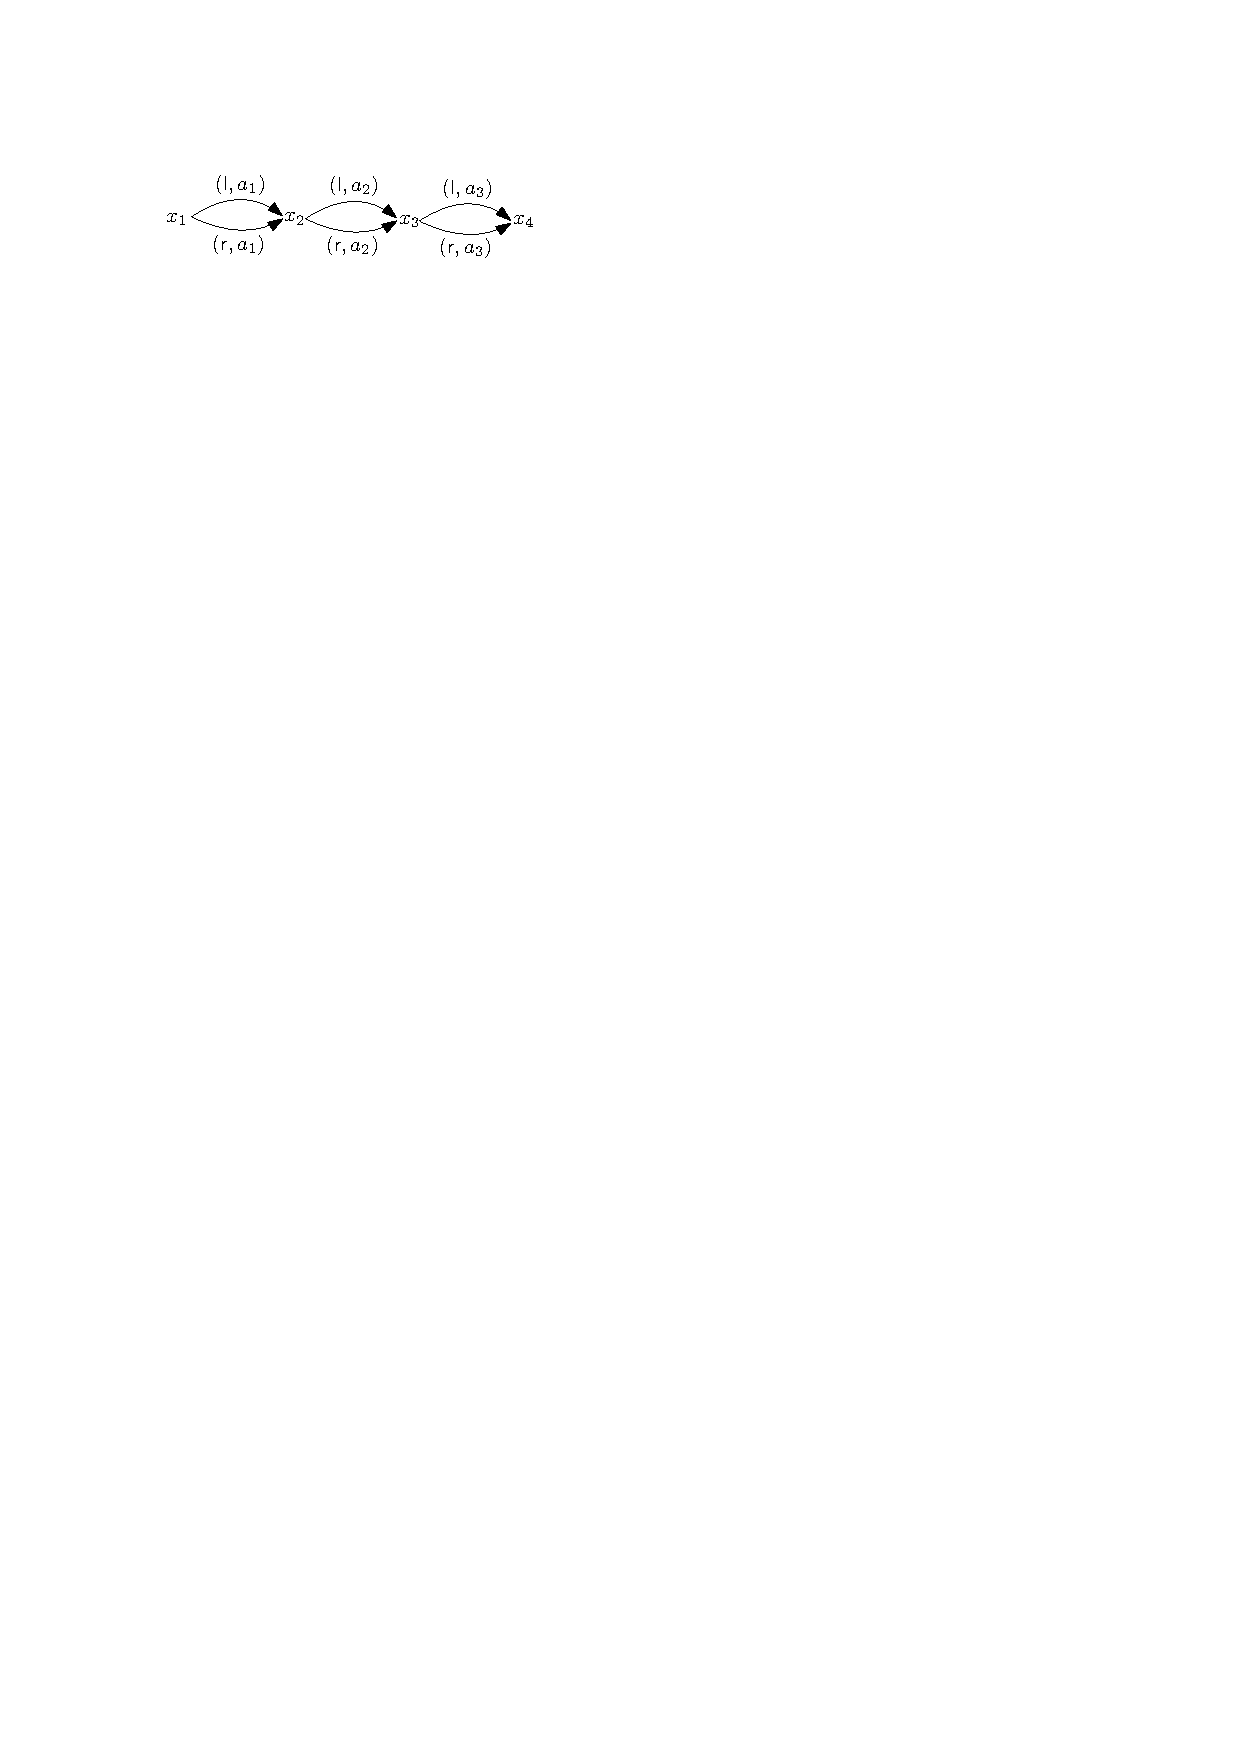
\includegraphics[scale=0.7]{dmdidx-example.pdf}
\end{center}
\caption{The diamond index  and the number of paths in $G_C$}\label{fig-dmdidx-exmp}
\end{figure}
\end{example}

In Section~\ref{sec:replaceallsl}--\ref{sec:replaceallre}, we will apply a refined analysis of the complexity of the decision procedures for proving Theorem~\ref{thm-main} and get the following results.

\begin{corollary}\label{cor-pspace}
The satisfiability problem is PSPACE-complete for the following fragments of $\strline[\replaceall]$:
\begin{itemize}
\item the single-letter case, plus the condition that the diamond indices of the dependency graphs are bounded by a constant $c$, 
%
\item the constant-string case, plus the condition that the $\rpleft$-lengths of the dependency graphs are bounded by a constant $c$, 

%
\item the regular-expression case, plus the condition that the $\rpleft$-lengths of the dependency graphs are at most $1$.
\end{itemize}
\end{corollary}

Corollary~\ref{cor-pspace} partially justifies our choice to present the decision procedures for the single-letter, constant-string, and regular-expression case separately. Intuitively, when the pattern parameters of $\replaceall$ terms become less restrictive, the decision procedures become more involved, and more constraints should be put on the dependency graphs in order to achieve the PSPACE upper bound. The PSPACE lower bound follows from the observation that the nonemptiness of the intersection of the regular expressions $e_1, \cdots, e_n$ over the alphabet $\{0,1\}$, which is a PSPACE-complete problem, can be reduced to the satisfiability of the formula $y = \replaceall((a b)^n, a, x) \wedge x \in (0+1)^\ast \wedge y \in e_1 \circ b  \circ \cdots \circ b \circ e_n$ (where $a, b \not \in \{0,1\}$), which belongs to all fragments in Corollary~\ref{cor-pspace}.\zhilin{Remark for the pspace lower bound, please check.}

%The proof of Theorem~\ref{thm-main} utilises a concept of dependency graphs defined below.



%Therefore,  in the following, without loss of generality, we assume that 
%in each $\strline[\replaceall]$ constraint $C=\varphi \wedge \psi$, the concatenation symbol $\concat$ does not occur in $\varphi$. 
 



%%%%%%%%%%%%%%%%%%%%%%%%%%%%%%%%%%%%%%%%%%%%%%%%%%%%%%%

\section{String-Manipulating Programs with Numeric Conditions}\label{sec:logic}

%!TEX root = main.tex

We consider symbolic execution of string-manipulating programs with numeric conditions (abbreviated as {\slint}), defined by the following rules, 
%
\[
\begin{array}{l c l}
S &::= &  x:= y \concat z \mid x:= \replaceall_{e,u}(y) \mid   x:=\reverse(y) \mid x:=\NFT(y) \mid \\
& & x := \substring(y, t_1, t_2)  \mid \ASSERT{\varphi}  \mid S;S, \\
\varphi &::= & x \in \NFA \mid t_1\ o\ t_2 \mid \varphi \vee \varphi \mid \varphi \wedge \varphi,
\end{array}
\]
where $e$ is a regular expression over $\Sigma$, $u \in \Sigma^*$, $\NFT$ is an FFT,  $\NFA$ is an NFA, $o \in \{=, \neq, \ge, \le, >, <\}$, and $t_1,t_2$ are integer terms defined by the following rules,
\[
t  ::= i \mid c \mid \length(x) \mid \indexof_v(x, i) \mid  ct  \mid t + t, \mbox{ where } c \in \Int, v \in \Sigma^+.
\]
%
%\[
%\begin{array}{l c l}
%t  &::=& i \mid c \mid \length(x) \mid \indexof_u(x, i) \mid  ct  \mid t + t,   \\
%S &::= &  x:= y \concat z \mid x:= \replaceall_{e,u}(y) \mid   x:=\reverse(y) \mid x:=\NFT(y) \mid \\
%& & x := \substring(y, t_1, t_2)  \mid S;S, \\
%A_r & ::= & x \in \NFA \mid A_r \wedge A_r,\\
%A_i & ::= & t\ o\ t \mid A_i \wedge A_i  \mid A_i \vee A_i,\\
%A & ::= &   A_r \wedge A_i,
%\end{array}
%\]
We require that the string-manipulating programs are in the {\bf single static assignment (SSA) form}. Note that the SSA form imposes restrictions only on the assignment statements, but not on the assertions. %conditional statements. 
%\tl{what does conditional statement mean? you mean assertions?}\zhilin{yes, I mean assertions. But actually they are not assertions we usually talk about, they are more like the conditions in the if-the-else statement.}
A string variable $x$ in a {\slint} program $S$ is called an \emph{input string variable} of $S$ if it does not appear on the left-hand side of the assignment statements of $S$. A variable in $S$ is called an \emph{input variable}  if it is either an input string variable or an integer variable.

\paragraph*{Semantics.}
The semantics of {\slint} is explained as follows. %mostly%self-explanatory, 
%if we know the semantics of the string-manipulating functions in {\slint}, 
%defined below. \tl{the semantics is not quite formal, so we may just **explain** them}
\begin{itemize}
\item The assignment $x:=y \cdot z$ denotes that $x$ is the concatenation of two strings $y$ and $z$.

\item The assignment $x:=\replaceall_{e,u}(y)$ denotes that $x$ is the string obtained by replacing all occurrences of $e$ in $y$ with $u$, where the \emph{leftmost and longest} matching of $e$ is used. For instance, $\replaceall_{(ab)^+,c}(aababaab) =ac \cdot \replaceall_{(ab)^+,c}(aab)= acac$, since the leftmost and longest matching of $(ab)^+$ in $aababaab$ is $abab$. Here we require that the language defined by $e$ does \emph{not} contain the empty string, in order to avoid the troublesome definition of the semantics of the matching of the empty string. We refer the reader to \cite{CCH+18} for the formal semantics of the $\replaceall$ function.
%
\item The assignment $x:=\reverse(y)$ denotes that $x$ is the reverse of $y$.
%
\item The assignment $x:=\NFT(y)$ denotes that $(y,x) \in \Tran(\NFT)$. %$x$ is an output of some accepting run of $\NFT$ on $y$.
%
\item The assignment $x:=\substring(y, t_1, t_2)$ denotes that $x$ is equal to the return value of $\substring(y, t_1, t_2)$, where 

\[ \substring(y, t_1, t_2)=
\begin{cases}
\epsilon & \mbox{if }t_1<0\vee t_1 \ge |y| \vee t_2=0 \\
y[t_1, \min\{t_1+t_2-1, |y|-1\}] & o/w
\end{cases}
\]
 %the substring of $y$ that begins at the position $t_1$ and extends to the length $t_2$. 
%$\substring(y, t_1, t_2)$ returns the empty string,  if $t_1$ is negative or $t_1$ is greater than or equal to the length of $y$, otherwise, if $t_2=0$, then it returns the empty string, otherwise, it returns the substring of $y$ from the position $t_1$ to the position $t_1+t_2-1$ (or to the last letter of $y$ if the length of $y$ is strictly less than $t_1+t_2$).  
For instance, $\substring(abaab, -1,1)=\varepsilon$, $\substring(abaab, 3,0)=\varepsilon$, $\substring(abaab, 3,2)=ab$, and $\substring(abaab, 3,3)=ab$.
%\tl{check the starting position}
%Note here we require that $t_2 \ge 0$. 
%
\item The conditional statement $\ASSERT{x \in \NFA}$ denotes that $x$ belongs to $\Lang(\NFA)$.
%
\item The conditional statement $\ASSERT{t_1 \ o\ t_2}$ denotes that the value of $t_1$ is equal to (not equal to, \dots) that of $t_2$, if $o\in \{ =, \neq, \geq, >, \leq, < \}$.
%
\item The integer term $\length(x)$ denotes the length of $x$. 
%
\item The function $\indexof_v(x, i)$ returns the starting position of the first occurrence of $v$ in $x$ after the position $i$, if such an occurrence exists, and $-1$ otherwise. Note that if $i<0$, then $\indexof_v(x, i)$ returns $\indexof_v(x, 0)$, and if $i \ge \length(x)$, then $\indexof_v(x, i)$ returns $-1$. For instance, $\indexof_{ab}(aaba, -1) = 1$, $\indexof_{ab}(aaba, 1) = 1$, $\indexof_{ab}(aaba, 2)=-1$, and $\indexof_{ab}(aaba, 4)=-1$.
\end{itemize}

\begin{example}\label{exmp:logic}
%\zhilin{adjust to the running example in the introduction}
After adapting the syntax of the program corresponding to the ``if'' branch of {\tt urlXssSanitise(url)} in Example~\ref{exmp:running}, we get the following {\slint} program $S$,
\[ 
\begin{array}{l}
    \ASSERT{\mathtt{prothostpath} \in \NFA_\varepsilon}; \ASSERT{\mathtt{querfrag} \in \NFA_\varepsilon};\\
    \mathtt{url1} := \NFT_{\rm trim}(\mathtt{url}); \ASSERT{\mathtt{qmarkpos} = \indexof_?(\mathtt{url1},0)};\\
    \ASSERT{\mathtt{sharppos} = \indexof_{\#}(\mathtt{url1}, 0)}; \ASSERT{\mathtt{qmarkpos} >= 0};\\ 
    \mathtt{prothostpath1} := \substring(\mathtt{url1}, 0, \mathtt{qmarkpos});\\
   \mathtt{querfrag1} := \substring(\mathtt{url1, qmarkpos}, \length(\mathtt{url1}) - \mathtt{qmarkpos});\\
    \mathtt{querfrag2} := \replaceall_{\mathtt{<script>+javascript:},\ \varepsilon}(\mathtt{querfrag1});\\
    \mathtt{url2} := \mathtt{prothostpath1} \concat \mathtt{querfrag2};\\
    \ASSERT{\mathtt{querfrag2} \in \NFA_{\mathtt{<script>+javascript:}}}
\end{array}
\]
where $\NFA_\varepsilon$ is the NFA defining $\{\varepsilon\}$, $\NFT_{\rm trim}$ is an NFT to model the sanitisation operation {\tt trim()}, and $\NFA_{\mathtt{<script>+javascript:}}$ is the NFA defining $\{\mbox{\tt <script>, javascript:}\}$. 
%
%
%In particular, {\tt qmarkpos = url1.indexof('?')} in $S$ is transformed into $\ASSERT{{\tt qmarkpos = \indexof_{?}(url1,0)}}$, and {\tt url1=url.trim()} is adapted into ${\tt url1}:=\NFT_{\rm trim}({\tt url})$, where $\NFT_{\rm trim}$ is an NFT to model the sanitisation operation {\tt trim()}, moreover,  
%{\tt
%\begin{minted}{javascript}
%querfrag2 = querfrag1.replace(/<script>|javascript:/g, '')
%\end{minted}
%}
%is changed into the statement ${\tt querfrag2}:=\replaceall_{e,\varepsilon}({\tt querfrag1})$, where $e$ is the regular expression {\tt $<$script$>$+javascript:} (where $+$ is the alternation).
%\[
%\begin{array}{l}
%y := \replaceall_{\Sigma \setminus ), \varepsilon}(x); z:= \replaceall_{\Sigma \setminus (, \varepsilon}(x);\\
%\ASSERT{\length(y) = \length(z)}; \ASSERT{\indexof_{"("}(x,0) < \indexof_{")"}(x,0)}
%\end{array}
%\] 
%is in {\slint}, where $\Sigma \setminus a$ (where $a \in \{(,)\}$) is the regular expression $(+b)_{b \in \Sigma \setminus \{a\}}$. Intuitively the program states that $x$ contains the same number of occurrences of ``('' and ``)''; and the first occurrence of ``('' is before the first occurrence of ``)''.
\end{example}


\begin{remark}
Note that %to ease the notation, we allow only variables in the string parameters of string operations in {\slint}, and 
for simplicity, strictly speaking, string constants are not allowed in the assignments. %therein. 
For instance, %string variables, instead of string constants, are required to appear as the string parameters of $\reverse$. This is not a real restriction, since 
$x:=\reverse({\mbox``}abc\mbox{''})$ is disallowed. However, this is not a real restriction because it can be written as $x:=\reverse(y); \ASSERT{y \in \NFA_{abc}}$, where $y$ is a fresh variable and $\NFA_{abc}$ is the NFA which accepts ``$abc$''  only.
\end{remark}


\begin{remark}
The function $\replaceall_{e,u}$ can be seen as a special case of FFT, although the transformation into the equivalent FFT $\NFT_{\replaceall_{e,u}}$ may incur an exponential blowup \cite{CCH+18}.
\end{remark}

To exemplify the expressiveness of our language, we note that the function $\charat(x, i)$ which returns $x[i]$ (i.e., the character of $x$ at the position $i$) can be seen as a special case of $\substring$, namely $\charat(x, i) \equiv \substring(x, i, 1)$. Furthermore, string inequality $x \neq y$ can be expressed as the following {\slint} program (denoted by $S_{x \neq y}$)
\[
\begin{array}{l}
z_1:=\charat(x,i); z_2 := \charat(y,i); \\
\ASSERT{\length(x) \neq \length(y) \vee \bigvee_{a \in \Sigma} (z_1 \in \NFA_a \wedge z_2 \in \NFA_{\Sigma \setminus a})},
\end{array}
\] 
where $z_1,z_2$ are two freshly introduced string variables, and $\NFA_a$ (resp. $\NFA_{\Sigma \setminus a}$) is the NFA accepting $\{a\}$ (resp. $\Sigma \setminus \{a\}$). Intuitively, two strings are different if their lengths are different or otherwise, there exists some position where the characters of the two strings are different.
 



%The logic {\slint} is defined as straight-line fragment of the aforementioned string constraints, specifically, {\slint} is defined as the collection of the formulae $S \wedge A$ satisfying that {\bf $S$ is in single static assignment (SSA) form}.  Note that in {\slint}, the straight-line restriction is applied only on $S$, which contains only the assignments to string variables (but not integer variables). No restrictions are put on the integer constraints in $A_i$.

\paragraph*{Path feasibility problem.} Given a {\slint} program $S$, decide whether there are valuations of input variables so that $S$ can execute to the end.

%\medskip
%
%In the sequel, we are going to design a decision procedure for the path feasibility problem of {\slint} programs. We will first lay down the theoretical foundations of the decision procedure in the next section, where the concepts of regular languages and recognisable relations are extended.
















%%%%%%%%%%%%%%%%%%%%%%%%%%%%%%%%%%%%%%%%%
%%%%%%%%%%% The original abstract logic definition %%%%%%%%%%%%
%%%%%%%%%%% The original abstract logic definition %%%%%%%%%%%%
%%%%%%%%%%%%%%%%%%%%%%%%%%%%%%%%%%%%%%%%%
%%%%%%%%%%%%%%%%%%%%%%%%%%%%%%%%%%%%%%%%%

\hide{
The string logic {\slint} defined by the following rules% satisfies the two semantic conditions,
\[
\begin{array}{l c l}
t  &::=& i \mid c \mid \length(x) \mid \indexof_u(x, i) \mid  ct  \mid t + t,   \\
S &::= &  x:= y \concat z \mid x:= \replaceall_{e,u}(y) \mid   x:=\reverse(y) \mid x:=T(y) \mid \\
& & x := \substring(y, t_1, t_2)  \mid S;S, \\
A & ::= &   A_r \wedge A_i,\\
A_r & ::= & x \in \NFA \mid A_r \wedge A_r,\\
A_i & ::= & t\ o\ t \mid A_i \wedge A_i  \mid A_i \vee A_i,
\end{array}
\]
where  $u \in \Sigma^+$, $e$ is a regular expression, $T$ is a finite-state transducer, and $o \in \{=, \neq, \ge, \le, >, <\}$.

We consider two types of functions, string functions that return strings and integer functions that return integers. Specifically, we consider 
\begin{itemize}
\item string functions $f(x_1, \vec{i_1}, \cdots, x_k, \vec{i_k})$, where $f$ is of the arity $\Sigma^* \times \intnum^{n_1} \times \cdots \times \Sigma^* \times \intnum^{n_k} \rightarrow 2^{\Sigma^*}$, and
\item  integer functions $g(x_1, \vec{i_1}, \cdots, x_k, \vec{i_k})$, where $g$ is of the arity $\Sigma^* \times \intnum^{n_1} \times \cdots \times \Sigma^* \times \intnum^{n_k} \rightarrow 2^\intnum$.
\end{itemize} 
Note that $f$ and $g$ can be nondeterministic.
%\subsection{The abstract version}

We consider string constraints where the formulae are of the form $S \wedge A$ defined by the following rules,
\[
\begin{array}{l c l}
t  &::=& i \mid c \mid  g(x_1, \vec{t_1}, \cdots, x_k, \vec{t_k}) \mid ct \mid t + t,   \\
S &::= &  x:=f(x_1, \vec{t_1}, \cdots, x_k, \vec{t_k}) \mid S;S, \\
A_r & ::= & x \in \NFA  \mid A_r \wedge A_r, \\
A_i & ::= & t\ o\ t \mid A_i \wedge A_i \mid A_i \vee A_i,\\
A & ::= &   A_r \wedge A_i, 
\end{array}
\]
where $f$ is a string function and $g$ is an integer function, $\vec{t_j} = t_{j,1}, \cdots, t_{j, n_j}$ for each $j \in [k]$, $\NFA$ is a finite-state automaton, and $o \in \{=, \neq, \ge, \le, >, <\}$.

The logic {\slint} is defined as straight-line fragment of the aforementioned string constraints, specifically, {\slint} is defined as the collection of the formulae $S \wedge A$ satisfying that {\bf $S$ is in single static assignment (SSA) form}.  Note that in {\slint}, the straight-line restriction is applied only on $S$, which contains only the assignments to string variables (but not integer variables). No restrictions are put on the integer constraints in $A_i$.
\[
\begin{array}{l c l}
A & ::= &   A_r \wedge A_i, \\
A_r & ::= & x \in \NFA \mid A_r \wedge A_r,\\
A_i & ::= & t\ o\ t \mid A_i \wedge A_i  \mid A_i \vee A_i
\end{array}
\]
where  $u \in \Sigma^+$, $e$ is a regular expression, $T$ is a finite-state transducer, and $o \in \{=, \neq, \ge, \le, >, <\}$.
\tl{decide later whether $\replaceall_{e,u}(y)$ is needed here.}

%%%%%%%%%%%%%%%  Temporally commented out %%%%%%%%%%%%%%%%%%%%%%%
%\subsection{The abstract version}

%We consider two types of functions, string functions that return strings and integer functions that return integers. Specifically, we consider 
%\begin{itemize}
%	\item string functions $f(x_1, \vec{i_1}, \cdots, x_k, \vec{i_k})$, where $f$ is of the signature $\Sigma^* \times \intnum^{n_1} \times \cdots \times \Sigma^* \times \intnum^{n_k} \rightarrow 2^{\Sigma^*}$, and
%	\item  integer functions $g(x_1, \vec{i_1}, \cdots, x_k, \vec{i_k})$, where $g$ is of the signature $\Sigma^* \times \intnum^{n_1} \times \cdots \times \Sigma^* \times \intnum^{n_k} \rightarrow 2^\intnum$.
%\end{itemize} 
%Note that $f$ and $g$ can be nondeterministic.
%
%We consider string constraints where the formulae are of the form $S \wedge A$ defined by the following rules,
%\[
%\begin{array}{l c l}
%t  &::=& i \mid c \mid  g(x_1, \vec{t_1}, \cdots, x_k, \vec{t_k}) \mid ct \mid t + t,   \\
%S &::= &  x:=f(x_1, \vec{t_1}, \cdots, x_k, \vec{t_k}) \mid S;S, \\
%A_r & ::= & x \in \NFA  \mid A_r \wedge A_r, \\
%A_i & ::= & t\ o\ t \mid A_i \wedge A_i \mid A_i \vee A_i,\\
%A & ::= &   A_r \wedge A_i, 
%\end{array}
%\]
%where $f$ is a string function and $g$ is an integer function, $\vec{t_j} = t_{j,1}, \cdots, t_{j, n_j}$ for each $j \in [k]$, $\NFA$ is a finite-state automaton, and $o \in \{=, \neq, \ge, \le, >, <\}$.
%%%%%%%%%%%%%%%  Temporally commented out %%%%%%%%%%%%%%%%%%%%%%%

%The logic {\slint} is defined as straight-line fragment of the aforementioned string constraints, specifically, 
We assume that {\bf  string constraints %{\slint} is defined as the collection of the formulae $S \wedge A$ satisfying that 
$S$ are in single static assignment (SSA) form}.  %Note that in {\slint}, the straight-line restriction 
Note that it is applied  to $S$ only while it is remitted from the integer constraints in $A_i$. 
%which contains only the assignments to string variables (but not integer variables). No restrictions are put on the integer constraints in $A_i$.
%Intuitively speaking, the integer constraints in $S \wedge A$ are split into the integer assignments in $S$ where the right-hand side is of the form $g(x_1, \vec{i_1}, \cdots, x_k, \vec{i_k})$ and the constraints $t\ o\ t$ in $A$ where the integer functions $g$ do not occur.
%\begin{itemize}
%\item $S$ is in single static assignment (SSA) form,
%\item all the assignments $i: = t$ in $S$ satisfy that either $t$ is of the form $g(x_1, \vec{i_1}, \cdots, x_k, \vec{i_k})$, or $t$ contains no occurrences of the functions of the form $g(x_1, \vec{i_1}, \cdots, x_k, \vec{i_k})$, namely, $t$ is an integer term built from integer variables and constants ,
%
%\item $A$ contains no occurrences of the functions $g(x_1, \vec{i_1}, \cdots, x_k, \vec{i_k})$,
%
%\item all the string variables in $A$ also occur in $S$.
%\end{itemize} 

\begin{example}
The formula $x:= y \concat z \wedge y := \substring(y', \indexof(x, c), j)  \wedge y' \in (ab)^* \wedge z \in a^* c b^* \wedge   j = 2 \indexof(x, c)$ belongs to \slint.
\end{example}


\subsection{Semantics}

The semantics of  {\slint}  is largely self-explanatory. In particular, $\length(x)$ returns the length of string $x$, $\indexof_u(x, i)$ returns the first index of $u$ in $x$ after $i$. 

$\substring(y, t_1, t_2)$ returns the string of $y$ between $t_1$ and $t_2$. 

Intuitively, $\substring(x_1, i, j)$ returns the substring of $x_1$ starting from the position $i$ and ending at the position $j$ (assuming that $i  < j$), with the letter at the position $j$ excluded.

tbc...

%The replaceAll function encompasses two parameters: the first parameter is the subject string, and the second parameter is the replacement
%string whereas $u$ the
%second parameter is a pattern that is a regular expression, . For the semantics of replaceAll function, in particular when the pattern is a regular expression,
%we adopt the leftmost and longest matching. For instance, replaceAll(aababaab, (ab)+, c) = ac ·
%replaceAll(aab, (ab)+, c) = acac, since the leftmost and longest matching of (ab)+ in aababaab is
%abab. Herewe require that the language defined by the pattern parameter does not contain the empty
%string, in order to avoid the troublesome definition of the semantics of the matching of the empty
%string. We refer the reader to [Chen et al. 2018] for the formal semantics of the replaceAll function.
%To be consistent with the notations in this paper, for each regular expression e, we define the string
%function replaceAlle : Σ∗ × Σ∗ → Σ∗ such that for u,v ∈ Σ∗, replaceAlle (u,v) = replaceAll(u, e,v),
%and we write replaceAll(x, e,y) as replaceAlle (x,y).

In the next section, we specify the semantic conditions for {\slint} in order to achieve decision procedures. For this purpose, we need the concepts of cost-enriched regular languages and recognisable relations. 

%\section{The semantic conditions}
}

%%%%%%%%%%%%%%%%%%%%%%%%%%%%%%%%%%%%%%%%%%%%%%%%%%%%%%%%

\section{Automata-Theoretic Foundations}\label{sec:cefa}

%!TEX root = main.tex


%In this section, we introduce cost-enriched regular languages and recognisable relations, as the extensions of regular languages and recognisable relations, moreover, we investigate the decidability and complexity of a related decision problem, thus laying down the theoretical foundations of the decision procedure in the next section. 

\subsection{Cost-Enriched Regular Languages and Recognisable Relations} \label{sect:ce}

Let $k \in \Nat$ with $k > 0$. A \emph{$k$-cost-enriched string} is $(w, (n_1, \cdots, n_k))$ where $w$ is a string and $n_i \in \intnum$ for all $i \in [k]$. 
A \emph{$k$-cost-enriched language} $L$ is a subset of $\Sigma^* \times \intnum^k$. For our purpose, we identify a ``regular" fragment of cost-enriched languages as follows. 
%Note that all the cost-enriched strings in $L$ are associated with the same number of costs (i.e., $k$).

\begin{definition}[Cost-enriched regular languages]
Let $k \in \Nat$ with $k > 0$. A $k$-cost-enriched language is \emph{regular} (abbreviated as CERL) if it can be accepted by a \emph{cost-enriched finite automaton}. 

A cost-enriched finite automaton (CEFA) $\CEFA$ is a tuple $(Q, \Sigma, R, \delta, I, F)$ where 
\begin{itemize}
\item $Q, \Sigma, I, F$ are defined as in NFAs, 
%
\item $R=(r_1, \cdots, r_k)$ is a vector of (mutually distinct) \emph{cost registers}, 
%
\item $\delta$ is the transition relation which is a finite set of tuples $(q, a, q', \eta)$ where $q, q' \in Q$, $a \in \Sigma$, and %$\eta: R \rightarrow \intnum$ 
$\eta: R \rightarrow \Int$
is a cost register update function. \\
For convenience, we usually write $(q, a, q', \eta) \in \Delta$ as $q \xrightarrow{a, \eta} q'$.
\end{itemize}
%
A \emph{run} of $\CEFA$ on a $k$-cost-enriched string $(a_1 \cdots a_m, (n_1, \cdots,n_k))$ is a  transition sequence $q_0 \xrightarrow{a_1, \eta_1} q_1 \cdots q_{m-1} \xrightarrow{a_m, \eta_m} q_m$ such that $q_0 \in I$ and $n_i = \sum \limits_{1\leq j\leq m}\eta_j(r_i)$ for each $i \in [k]$ (Note that the initial values of cost registers are zero). The run is \emph{accepting} if $q_m \in F$. A $k$-cost-enriched string $(w, (n_1, \cdots,n_k))$ is accepted by $\CEFA$ if there is an accepting run of $\CEFA$ on $(w, (n_1, \cdots,n_k))$. In particular, $(\varepsilon, n)$ is accepted by $\CEFA$ if $n=0$ and $I\cap F \neq \emptyset$.
The $k$-cost-enriched language defined by $\CEFA$, denoted by $\Lang(\CEFA)$, is the set of $k$-cost-enriched strings accepted by $\CEFA$. 
%A cost-enriched language $L \subseteq \Sigma^* \times \intnum^k$ is called a cost-enriched regular language (CERL) if there is a CEFA $\NFA$ such that $L = \Lang(\NFA)$.
\end{definition}
The \emph{size} of a CEFA $\CEFA=(Q, \Sigma, R, \delta, I, F)$, denoted by $|\CEFA|$, is defined as the sum of the sizes of its transitions, where the size of each transition $(q, a, q', \eta)$ is $\sum \limits_{r \in R} \lceil \log_2 (|\eta(r)|) \rceil +3$. Note here  the integer constants in $\CEFA$ are encoded in binary.

\begin{remark}
CEFAs can be seen as a variant of Cost Register Automata \cite{RLJ+13}, by admitting nondeterminism and discarding partial final cost functions. CEFAs are also closely related to monotonic counter machines \cite{LB16}. The main difference is that CEFAs discard guards in transitions and allow integers in cost updates, while monotonic counter machines allow guards in transitions but restrict the cost updates to being monotonic, i.e. $0,1$ only. Moreover, we explicitly define CEFAs as language acceptors for  cost-enriched languages.
\end{remark}

\begin{example}[CEFA for $\length$]\label{exm:len}
The string function $\length$ can be captured by CEFA. For any NFA $\NFA=(Q, \Sigma,  \delta, I, F)$, it is not difficult to see that the cost-enriched language $\{(w, \length(w)) \mid w\in \Lang(\NFA)\}$ is accepted by a CEFA, i.e., 
$(Q, \Sigma, (r_1), \delta', I, F)$  %$Q =I=F= \{q_0\}$, $R=(r_1)$, and 
such that for each $(q, a, q')\in \delta$, we let $(q, a, q', \eta)\in \delta'$, where $\eta(r_1) = 1$. 

For later use, we identify a special $\CEFA_{\rm len}= (\{q_0\}, \Sigma, (r_1), \{(q_0, a, q_0, \eta) \mid \eta(r_1) = 1\}, \{q_0\}, \{q_0\})$. In other words, $\CEFA_{\rm len}$ accepts $\{(w, \length(w)) \mid w\in \Sigma^*\}$.
%
%
%to denote the CEFA $(Q, \Sigma, (r_1), \delta', I, F)$ for the special NFA $\NFA$ such that $\Lang(\NFA)=\Sigma^*$, specifically, $\NFA_{\rm len} = (\{q_0\}, \Sigma, (r_1), \{(q_0, a, q_0, \eta) \mid \eta(r_1) = 1\}, \{q_0\}, \{q_0\})$.
%\tl{it is a bit vague; you mean for any RE $e$,  is a cerl?}
\end{example}

We can show that the function $\indexof_v(\cdot, \cdot)$ can be captured by CEFA as well, in the sense that, for any NFA $\NFA$ and constant string $v$, we can construct a CEFA %$\CEFA'$ such that 
accepting $\{(w, (n, \indexof_v(w, n)))\mid w\in \Lang(\NFA) \}$. %$R(\CEFA')=(r_1,r_2)$ and $\Lang(\CEFA')=\{(w, (n, \indexof_v(w, n)))\mid w\in \Lang(\NFA) \}$. 
The construction is slightly technical and can be found in Appendix, Section~\ref{appendix:cefa_indexof}.

For convenience, we use $\CEFA_{\indexof_v}$ which accepts $\{(w, (n, \indexof_v(w, n)))\mid w\in \Sigma^*, n \le \indexof_v(w, n) < |w| \}$. %to denote the constructed CEFA $\CEFA'$ for the special NFA $\NFA$ such that $\Lang(\NFA)=\Sigma^*$. 
Note that $\CEFA_{\indexof_v}$ does not model the corner cases in the semantics of $\indexof_v$, for instance, $\indexof_v(w, n) = -1$ if $v$ does not occur after the position $n$ in $w$.
In the sequel, we will exemplify the construction of $\CEFA_{\indexof_v}$ for the special case that $v$ is a single letter.  

\begin{example}[CEFA for $\indexof_a$]\label{exm:indexof}
Let $a \in \Sigma$. Then  $\CEFA_{\indexof_a} = (\{(q_0, q_1, q_2)\}, \Sigma, (r_1,r_2), \delta_{\indexof_a}, \{q_0\}, \{q_2\})$, where $\delta_{\indexof_a}$ comprises the tuples
\begin{itemize}
\item $(q_0, b, q_0, \eta)$ such that $b \in \Sigma$, $\eta(r_1)=1$, $\eta(r_2)=1$,
%
\item $(q_0, b, q_1, \eta)$ such that $b \in \Sigma$, $\eta(r_1)=0$, $\eta(r_2) = 1$,
%
\item $(q_0, a, q_2, \eta)$ such that $\eta(r_1)=0$, $\eta(r_2) = 0$,
%
\item $(q_1, b, q_1, \eta)$ such that $b \in \Sigma \setminus \{a\}$, $\eta(r_1)=0$, $\eta(r_2)=1$,
%
\item $(q_1, a, q_2, \eta)$ such that $\eta(r_1)=0$, $\eta(r_2)=0$,
%
\item $(q_2, b, q_2, \eta)$ such that $b \in \Sigma$, $\eta(r_1)=0$, $\eta(r_2)=0$.
\end{itemize}
Intuitively, $r_1$ corresponds to the starting position $i$ of $\indexof_a(x, i)$, $r_2$ corresponds to the output of $\indexof_a(x, i)$, $q_0$ specifies that the current position is before $i$, $q_1$ specifies that the current position is after $i$, while $a$ has not occurred yet, and $q_2$ specifies that $a$ has occurred after $i$. 
\end{example}


Given two CEFAs $\CEFA_1 = ( Q_1, \Sigma, R_1, \delta_1, I_1, F_1)$ and $\CEFA_2 = (Q_2, \Sigma, \delta_2, R_2, I_2, F_2)$ with $R_1 \cap R_2 = \emptyset$ (where %the notation is abused a bit, viewing 
$R_1$ and $R_2$ are treated as sets), the product of $\CEFA_1$ and $\CEFA_2$, denoted by $\CEFA_1 \times \CEFA_2$, is defined as $(Q_1 \times Q_2, \Sigma, R_1 \cup R_2, \delta, I_1 \times I_2, F_1 \times F_2)$, where $\delta$ comprises the tuples $((q_1, q_2), \sigma, (q'_1, q'_2), \eta)$ such that $(q_1, \sigma, q'_1, \eta_1) \in \delta_1$, $(q_2, \sigma, q'_2, \eta_2) \in \delta_2$, and $\eta = \eta_1\cup \eta_2$.  %for some $\eta_1, \eta_2$.


For a CEFA $\CEFA$, we use $R(\CEFA)$ to denote the vector of cost registers occurring in $\CEFA$. %Note that cost registers of $\CEFA$ are simply integer variables to store costs in $\CEFA$.
%Moreover, for a CEFA $\NFA$ and 
Suppose $\CEFA$ is  CEFA with $R(\CEFA)=(r_1,\cdots, r_k)$ and $\vec{i} = (i_1,\cdots, i_k)$ with $R(\NFA) \cap \vec{i} = \emptyset$. We use $\CEFA[\vec{i}/R(\CEFA)]$ to denote the CEFA obtained from $\CEFA$ by simultaneously replacing $r_j$ with $i_j$ for $j \in [k]$. 

\smallskip

%Let $(k_1,\cdots, k_l) \in \Nat^l$ with $k_j > 0$ for every $j \in [l]$. A  $(k_1,\cdots, k_l)$-cost-enriched relation $\cR$ is a subset of $(\Sigma^* \times \intnum^{k_1}) \times \cdots (\Sigma^* \times \intnum^{k_l})$.

%%%%%%%%%%%%%%%%%%%%%%%%%%%%%%%%%%%%%%%%%%%%%%%%%%%%%%%%%%%%%%%%%%%%%%%%%%%%%%%%%%%%%%%%%%%%%%%
\begin{definition}[Cost-enriched recognisable relations]
Let $(k_1,\cdots, k_l) \in \Nat^l$ with $k_j > 0$ for every $j \in [l]$. A cost-enriched recognisable relation (CERR)  $\cR \subseteq (\Sigma^* \times \intnum^{k_1}) \times \cdots  \times (\Sigma^* \times \intnum^{k_l})$ is a finite union of products of CERLs. Formally,
	\[\cR = \bigcup \limits_{i=1}^n L_{i,1 } \times \cdots \times L_{i, l},\]
	where for every $j \in [l]$, $L_{i,j} \subseteq \Sigma^* \times \intnum^{k_j}$ is a CERL. 
	A CEFA representation of $\cR$ is a collection of CEFA tuples $(\CEFA_{i,1}, \cdots, \CEFA_{i,l})_{i \in [n]}$ such that $\Lang(\CEFA_{i,j}) = L_{i,j}$ for every $i \in [n]$ and $j \in [l]$.
\end{definition}

\begin{example}\label{exm:CERR}
The relation 
\[\cR=\left\{((w_1, |w_1|), (w_2, |w_2|)) \mid  w_1 \in \Lang((aa)^*), w_2 \in \Lang(b(bb)^*), |w_1|+|w_2| \ge 2\right\}\] 
is a CERR since 
$\cR = L_{1,1} \times L_{1,2} \cup L_{2,1} \times L_{2,2}$, where 
\begin{itemize}
\item $L_{1,1}=\{(w_1, |w_1|) \mid w_1 \in \Lang((aa)^*)\}$, 
\item $L_{1,2}=\{(w_2, |w_2|) \mid  w_2 \in \Lang(bbb(bb)^*)\}$ , 
\item $L_{2,1}=\{(w_1, |w_1|) \mid w_1 \in \Lang(aa(aa)^*)\}$,  and
\item $L_{2,2}=\{(w_2, |w_2|) \mid  w_2 \in \Lang(b(bb)^*)\}$. 
\end{itemize}
Note that $L_{i,j}$ for $i,j\in[2]$ are CERLs, with corresponding CEFAs $\CEFA_{i,j}$ by  Example~\ref{exm:len}. It follows that %Moreover, 
$(\CEFA_{i,1}, \CEFA_{i,2})_{i \in [2]}$ gives a CEFA representation of $\cR$. %, where 
%\tl{to be simplified.}
%\begin{itemize}
%\item  $\CEFA_{1,1} = (\{p_0, p_1\}, \{a,b\}, (r_{1}), \delta_{1,1}, \{p_0\}, \{p_0\})$ defines $L_{1,1}$, such that $\delta_{1,1}= \{(p_0, a, p_1,\eta_1)$, $(p_1, a, p_0, \eta_1)\}$, with $\eta_1(r_{1})=1$,
%%
%\item $\CEFA_{1,2}=(\{q_0,q_1,q_2\}, \{a,b\}, (r_{2}), \delta_{1,2}, \{q_0\}, \{q_1\})$ defines $L_{1,2}$, such that $\delta_{1,2}=\{(q_0, b, q_1,\eta_2), (q_1, b, q_2, \eta_2), (q_2, b, q_1,\eta_2)\}$, with $\eta_2(r_{2})=1$,
%%
%\item $\CEFA_{2,1} = (\{p_0, p_1,p_2, p_3\}, \{a,b\}, (r_{1}), \delta_{2,1}, \{p_0\}, \{p_2\})$ defines $L_{2,1}$, such that $\delta_{2,1} = \{(p_0, a, p_1, \eta_1), (p_1, a, p_2, \eta_1), (p_2, a, p_3, \eta_1), (p_3, a, p_2, \eta_1)\}$, with $\eta_1(r_{1})=1$, and
%%
%\item $\CEFA_{2,2}=(\{q_0,q_1,q_2\}, \{a,b\}, (r_{2}), \delta_{2,2}, \{q_1\})$ defines $L_{2,2}$, such that $\delta_{2,2}= (q_0, b, q_1,\eta_2), (q_1, b, q_2, \eta_2), (q_2, b, q_1,\eta_2)\}$, with $\eta_2(r_{2})=1$.
%\end{itemize}
\end{example}

%\subsection{Satisfiability of Linear Integer Arithmetic Formula with respect to CEFAs}
%
%In the sequel, we consider a decision problem for CEFAs which will be used for the decision procedure of the path feasibility problem for {\slint} in the next section.
%
%\begin{definition}[{\lasat} Problem]\label{def-la-sat-cefa}
%	The satisfiability problem of LIA formulas w.r.t. CEFAs (abbreviated as {\lasat} problem) is defined as follows.
%	
%	\textbf{Input}: a given quantifier-free LIA formula $\phi$ and CEFAs $\CEFA_1,\cdots,\CEFA_m$, such that $\CEFA_i=(Q_i, \Sigma, R_i, \delta_i, I_i, F_i)$ for every $i\in [m]$, 
%  $R_i \cap R_j = \emptyset$ for every $1 \le i < j \le m$, and
% the free variables of $\phi$ are from $\bigcup_{i\in [m]} R_i$, 
% 
%Decide whether %$\phi$ is satisfiable w.r.t. $\CEFA_1, \cdots, \CEFA_m$, namely, whether 
%there are an assignment function $\theta: \bigcup \limits_{i \in [m]} R_i \rightarrow \Int$ and strings $w_1, \cdots, w_m$  
%	such that  $\phi[(\theta(R_i)/R_i)_{i \in [m]}]$ hold and $(w_i, \theta(R_i)) \in \Lang(\NFA_i)$ for every $i \in [m]$.
%\end{definition}
%%Note that in Definition~\ref{def-la-sat-cefa}, registers in $\NFA_i$'s may intersect. 
%
%\begin{example}
%Let $\phi \equiv r_1 = r_2$ and $\CEFA_{1,1}, \CEFA_{1,2}$ be two CEFAs in Example~\ref{exm:CERR} defining $L_{1,1}, L_{1,2}$ respectively. (Recall that $R(\CEFA_{1,1})=(r_1)$ and $R(\CEFA_{1,2})=(r_2)$.) Then it is easy to see that $\phi$ is unsatisfiable w.r.t. $\CEFA_{1,1}$ and $\CEFA_{1,2}$, since for each $(w_1, n_1) \in L_{1,1}$, $n_1$ must be even, while for each $(w_2, n_2) \in L_{1,2}$, $n_2$ must be odd. Hence $n_1$ and $n_2$ cannot be equal.
%\end{example}
%
%\begin{theorem}\label{thm-la-sat-cefa}
%	The {\lasat} problem is NP-complete.
%\end{theorem}
%The proof is given in Appendix, Section~\ref{appendix:thm-la-sat-cefa}.

%%%%%%%%%%%%%%%%%%%%%%%%%%%%%%%%%%%%%%%%%%%%%%%%%%%%%%%%

\section{Decision Procedure}\label{sec:dec}

%!TEX root = main.tex

%In this section, we show the main result of this paper. 

%\begin{theorem}\label{thm-main}
%The path feasibility of {\slint} programs is $\expspace$-complete.  
%\end{theorem}
%%
%The lower bound of Theorem~\ref{thm-main} follows from Theorem~5 in \cite{LB16}, where the satisfiability of straight-line sting constraints with concatenation and finite transducers is shown to be the $\expspace$-complete.
%
%For the upper bound, we will design a decision procedure for the path feasibility problem of {\slint} programs, based on the concepts of CERLs and CERRs introduced Section~\ref{sec:cefa}.
%\zhilin{I think we can use Proposition 16 in \cite{LB16} to get the expspace upper bound. But to use this result, we need restrict CEFA to monotonic counter automata.}

In this section, we present a decision procedure for the path feasibility problem of {\slint}. A distinguished feature of the decision procedure is that it carries out backward computation which is local and can be done in a modular way. To support this, we extend the regular language with quantitative information of the strings in the language, giving rise to cost-enriched regular language and corresponding finite automata (Section \ref{sect:ce}). The crux of the decision procedure is thus to %we will 
show that the %cost-enriched 
pre-images of cost-enriched regular languages under the string operations in {\slint} (i.e., concatenation $\concat$, $\replaceall_{e,u}$, $\reverse$, NFTs $\NFT$, and $\substring$) are representable by so called recognizable relations (Section \ref{sect:pre}). \tl{will improve writing later}

%!TEX root = main.tex


%In this section, we introduce cost-enriched regular languages and recognisable relations, as the extensions of regular languages and recognisable relations, moreover, we investigate the decidability and complexity of a related decision problem, thus laying down the theoretical foundations of the decision procedure in the next section. 

\subsection{Cost-Enriched Regular Languages and Recognisable Relations} \label{sect:ce}

Let $k \in \Nat$ with $k > 0$. A \emph{$k$-cost-enriched string} is $(w, (n_1, \cdots, n_k))$ where $w$ is a string and $n_i \in \intnum$ for all $i \in [k]$. 
A \emph{$k$-cost-enriched language} $L$ is a subset of $\Sigma^* \times \intnum^k$. For our purpose, we identify a ``regular" fragment of cost-enriched languages as follows. 
%Note that all the cost-enriched strings in $L$ are associated with the same number of costs (i.e., $k$).

\begin{definition}[Cost-enriched regular languages]
Let $k \in \Nat$ with $k > 0$. A $k$-cost-enriched language is \emph{regular} (abbreviated as CERL) if it can be accepted by a \emph{cost-enriched finite automaton}. 

A cost-enriched finite automaton (CEFA) $\CEFA$ is a tuple $(Q, \Sigma, R, \delta, I, F)$ where 
\begin{itemize}
\item $Q, \Sigma, I, F$ are defined as in NFAs, 
%
\item $R=(r_1, \cdots, r_k)$ is a vector of (mutually distinct) \emph{cost registers}, 
%
\item $\delta$ is the transition relation which is a finite set of tuples $(q, a, q', \eta)$ where $q, q' \in Q$, $a \in \Sigma$, and %$\eta: R \rightarrow \intnum$ 
$\eta: R \rightarrow \Int$
is a cost register update function. \\
For convenience, we usually write $(q, a, q', \eta) \in \Delta$ as $q \xrightarrow{a, \eta} q'$.
\end{itemize}
%
A \emph{run} of $\CEFA$ on a $k$-cost-enriched string $(a_1 \cdots a_m, (n_1, \cdots,n_k))$ is a  transition sequence $q_0 \xrightarrow{a_1, \eta_1} q_1 \cdots q_{m-1} \xrightarrow{a_m, \eta_m} q_m$ such that $q_0 \in I$ and $n_i = \sum \limits_{1\leq j\leq m}\eta_j(r_i)$ for each $i \in [k]$ (Note that the initial values of cost registers are zero). The run is \emph{accepting} if $q_m \in F$. A $k$-cost-enriched string $(w, (n_1, \cdots,n_k))$ is accepted by $\CEFA$ if there is an accepting run of $\CEFA$ on $(w, (n_1, \cdots,n_k))$. In particular, $(\varepsilon, n)$ is accepted by $\CEFA$ if $n=0$ and $I\cap F \neq \emptyset$.
The $k$-cost-enriched language defined by $\CEFA$, denoted by $\Lang(\CEFA)$, is the set of $k$-cost-enriched strings accepted by $\CEFA$. 
%A cost-enriched language $L \subseteq \Sigma^* \times \intnum^k$ is called a cost-enriched regular language (CERL) if there is a CEFA $\NFA$ such that $L = \Lang(\NFA)$.
\end{definition}
The \emph{size} of a CEFA $\CEFA=(Q, \Sigma, R, \delta, I, F)$, denoted by $|\CEFA|$, is defined as the sum of the sizes of its transitions, where the size of each transition $(q, a, q', \eta)$ is $\sum \limits_{r \in R} \lceil \log_2 (|\eta(r)|) \rceil +3$. Note here  the integer constants in $\CEFA$ are encoded in binary.

\begin{remark}
CEFAs can be seen as a variant of Cost Register Automata \cite{RLJ+13}, by admitting nondeterminism and discarding partial final cost functions. CEFAs are also closely related to monotonic counter machines \cite{LB16}. The main difference is that CEFAs discard guards in transitions and allow integers in cost updates, while monotonic counter machines allow guards in transitions but restrict the cost updates to being monotonic, i.e. $0,1$ only. Moreover, we explicitly define CEFAs as language acceptors for  cost-enriched languages.
\end{remark}

\begin{example}[CEFA for $\length$]\label{exm:len}
The string function $\length$ can be captured by CEFA. For any NFA $\NFA=(Q, \Sigma,  \delta, I, F)$, it is not difficult to see that the cost-enriched language $\{(w, \length(w)) \mid w\in \Lang(\NFA)\}$ is accepted by a CEFA, i.e., 
$(Q, \Sigma, (r_1), \delta', I, F)$  %$Q =I=F= \{q_0\}$, $R=(r_1)$, and 
such that for each $(q, a, q')\in \delta$, we let $(q, a, q', \eta)\in \delta'$, where $\eta(r_1) = 1$. 

For later use, we identify a special $\CEFA_{\rm len}= (\{q_0\}, \Sigma, (r_1), \{(q_0, a, q_0, \eta) \mid \eta(r_1) = 1\}, \{q_0\}, \{q_0\})$. In other words, $\CEFA_{\rm len}$ accepts $\{(w, \length(w)) \mid w\in \Sigma^*\}$.
%
%
%to denote the CEFA $(Q, \Sigma, (r_1), \delta', I, F)$ for the special NFA $\NFA$ such that $\Lang(\NFA)=\Sigma^*$, specifically, $\NFA_{\rm len} = (\{q_0\}, \Sigma, (r_1), \{(q_0, a, q_0, \eta) \mid \eta(r_1) = 1\}, \{q_0\}, \{q_0\})$.
%\tl{it is a bit vague; you mean for any RE $e$,  is a cerl?}
\end{example}

We can show that the function $\indexof_v(\cdot, \cdot)$ can be captured by CEFA as well, in the sense that, for any NFA $\NFA$ and constant string $v$, we can construct a CEFA %$\CEFA'$ such that 
accepting $\{(w, (n, \indexof_v(w, n)))\mid w\in \Lang(\NFA) \}$. %$R(\CEFA')=(r_1,r_2)$ and $\Lang(\CEFA')=\{(w, (n, \indexof_v(w, n)))\mid w\in \Lang(\NFA) \}$. 
The construction is slightly technical and can be found in Appendix, Section~\ref{appendix:cefa_indexof}.

For convenience, we use $\CEFA_{\indexof_v}$ which accepts $\{(w, (n, \indexof_v(w, n)))\mid w\in \Sigma^*, n \le \indexof_v(w, n) < |w| \}$. %to denote the constructed CEFA $\CEFA'$ for the special NFA $\NFA$ such that $\Lang(\NFA)=\Sigma^*$. 
Note that $\CEFA_{\indexof_v}$ does not model the corner cases in the semantics of $\indexof_v$, for instance, $\indexof_v(w, n) = -1$ if $v$ does not occur after the position $n$ in $w$.
In the sequel, we will exemplify the construction of $\CEFA_{\indexof_v}$ for the special case that $v$ is a single letter.  

\begin{example}[CEFA for $\indexof_a$]\label{exm:indexof}
Let $a \in \Sigma$. Then  $\CEFA_{\indexof_a} = (\{(q_0, q_1, q_2)\}, \Sigma, (r_1,r_2), \delta_{\indexof_a}, \{q_0\}, \{q_2\})$, where $\delta_{\indexof_a}$ comprises the tuples
\begin{itemize}
\item $(q_0, b, q_0, \eta)$ such that $b \in \Sigma$, $\eta(r_1)=1$, $\eta(r_2)=1$,
%
\item $(q_0, b, q_1, \eta)$ such that $b \in \Sigma$, $\eta(r_1)=0$, $\eta(r_2) = 1$,
%
\item $(q_0, a, q_2, \eta)$ such that $\eta(r_1)=0$, $\eta(r_2) = 0$,
%
\item $(q_1, b, q_1, \eta)$ such that $b \in \Sigma \setminus \{a\}$, $\eta(r_1)=0$, $\eta(r_2)=1$,
%
\item $(q_1, a, q_2, \eta)$ such that $\eta(r_1)=0$, $\eta(r_2)=0$,
%
\item $(q_2, b, q_2, \eta)$ such that $b \in \Sigma$, $\eta(r_1)=0$, $\eta(r_2)=0$.
\end{itemize}
Intuitively, $r_1$ corresponds to the starting position $i$ of $\indexof_a(x, i)$, $r_2$ corresponds to the output of $\indexof_a(x, i)$, $q_0$ specifies that the current position is before $i$, $q_1$ specifies that the current position is after $i$, while $a$ has not occurred yet, and $q_2$ specifies that $a$ has occurred after $i$. 
\end{example}


Given two CEFAs $\CEFA_1 = ( Q_1, \Sigma, R_1, \delta_1, I_1, F_1)$ and $\CEFA_2 = (Q_2, \Sigma, \delta_2, R_2, I_2, F_2)$ with $R_1 \cap R_2 = \emptyset$ (where %the notation is abused a bit, viewing 
$R_1$ and $R_2$ are treated as sets), the product of $\CEFA_1$ and $\CEFA_2$, denoted by $\CEFA_1 \times \CEFA_2$, is defined as $(Q_1 \times Q_2, \Sigma, R_1 \cup R_2, \delta, I_1 \times I_2, F_1 \times F_2)$, where $\delta$ comprises the tuples $((q_1, q_2), \sigma, (q'_1, q'_2), \eta)$ such that $(q_1, \sigma, q'_1, \eta_1) \in \delta_1$, $(q_2, \sigma, q'_2, \eta_2) \in \delta_2$, and $\eta = \eta_1\cup \eta_2$.  %for some $\eta_1, \eta_2$.


For a CEFA $\CEFA$, we use $R(\CEFA)$ to denote the vector of cost registers occurring in $\CEFA$. %Note that cost registers of $\CEFA$ are simply integer variables to store costs in $\CEFA$.
%Moreover, for a CEFA $\NFA$ and 
Suppose $\CEFA$ is  CEFA with $R(\CEFA)=(r_1,\cdots, r_k)$ and $\vec{i} = (i_1,\cdots, i_k)$ with $R(\NFA) \cap \vec{i} = \emptyset$. We use $\CEFA[\vec{i}/R(\CEFA)]$ to denote the CEFA obtained from $\CEFA$ by simultaneously replacing $r_j$ with $i_j$ for $j \in [k]$. 

\smallskip

%Let $(k_1,\cdots, k_l) \in \Nat^l$ with $k_j > 0$ for every $j \in [l]$. A  $(k_1,\cdots, k_l)$-cost-enriched relation $\cR$ is a subset of $(\Sigma^* \times \intnum^{k_1}) \times \cdots (\Sigma^* \times \intnum^{k_l})$.

%%%%%%%%%%%%%%%%%%%%%%%%%%%%%%%%%%%%%%%%%%%%%%%%%%%%%%%%%%%%%%%%%%%%%%%%%%%%%%%%%%%%%%%%%%%%%%%
\begin{definition}[Cost-enriched recognisable relations]
Let $(k_1,\cdots, k_l) \in \Nat^l$ with $k_j > 0$ for every $j \in [l]$. A cost-enriched recognisable relation (CERR)  $\cR \subseteq (\Sigma^* \times \intnum^{k_1}) \times \cdots  \times (\Sigma^* \times \intnum^{k_l})$ is a finite union of products of CERLs. Formally,
	\[\cR = \bigcup \limits_{i=1}^n L_{i,1 } \times \cdots \times L_{i, l},\]
	where for every $j \in [l]$, $L_{i,j} \subseteq \Sigma^* \times \intnum^{k_j}$ is a CERL. 
	A CEFA representation of $\cR$ is a collection of CEFA tuples $(\CEFA_{i,1}, \cdots, \CEFA_{i,l})_{i \in [n]}$ such that $\Lang(\CEFA_{i,j}) = L_{i,j}$ for every $i \in [n]$ and $j \in [l]$.
\end{definition}

\begin{example}\label{exm:CERR}
The relation 
\[\cR=\left\{((w_1, |w_1|), (w_2, |w_2|)) \mid  w_1 \in \Lang((aa)^*), w_2 \in \Lang(b(bb)^*), |w_1|+|w_2| \ge 2\right\}\] 
is a CERR since 
$\cR = L_{1,1} \times L_{1,2} \cup L_{2,1} \times L_{2,2}$, where 
\begin{itemize}
\item $L_{1,1}=\{(w_1, |w_1|) \mid w_1 \in \Lang((aa)^*)\}$, 
\item $L_{1,2}=\{(w_2, |w_2|) \mid  w_2 \in \Lang(bbb(bb)^*)\}$ , 
\item $L_{2,1}=\{(w_1, |w_1|) \mid w_1 \in \Lang(aa(aa)^*)\}$,  and
\item $L_{2,2}=\{(w_2, |w_2|) \mid  w_2 \in \Lang(b(bb)^*)\}$. 
\end{itemize}
Note that $L_{i,j}$ for $i,j\in[2]$ are CERLs, with corresponding CEFAs $\CEFA_{i,j}$ by  Example~\ref{exm:len}. It follows that %Moreover, 
$(\CEFA_{i,1}, \CEFA_{i,2})_{i \in [2]}$ gives a CEFA representation of $\cR$. %, where 
%\tl{to be simplified.}
%\begin{itemize}
%\item  $\CEFA_{1,1} = (\{p_0, p_1\}, \{a,b\}, (r_{1}), \delta_{1,1}, \{p_0\}, \{p_0\})$ defines $L_{1,1}$, such that $\delta_{1,1}= \{(p_0, a, p_1,\eta_1)$, $(p_1, a, p_0, \eta_1)\}$, with $\eta_1(r_{1})=1$,
%%
%\item $\CEFA_{1,2}=(\{q_0,q_1,q_2\}, \{a,b\}, (r_{2}), \delta_{1,2}, \{q_0\}, \{q_1\})$ defines $L_{1,2}$, such that $\delta_{1,2}=\{(q_0, b, q_1,\eta_2), (q_1, b, q_2, \eta_2), (q_2, b, q_1,\eta_2)\}$, with $\eta_2(r_{2})=1$,
%%
%\item $\CEFA_{2,1} = (\{p_0, p_1,p_2, p_3\}, \{a,b\}, (r_{1}), \delta_{2,1}, \{p_0\}, \{p_2\})$ defines $L_{2,1}$, such that $\delta_{2,1} = \{(p_0, a, p_1, \eta_1), (p_1, a, p_2, \eta_1), (p_2, a, p_3, \eta_1), (p_3, a, p_2, \eta_1)\}$, with $\eta_1(r_{1})=1$, and
%%
%\item $\CEFA_{2,2}=(\{q_0,q_1,q_2\}, \{a,b\}, (r_{2}), \delta_{2,2}, \{q_1\})$ defines $L_{2,2}$, such that $\delta_{2,2}= (q_0, b, q_1,\eta_2), (q_1, b, q_2, \eta_2), (q_2, b, q_1,\eta_2)\}$, with $\eta_2(r_{2})=1$.
%\end{itemize}
\end{example}

%\subsection{Satisfiability of Linear Integer Arithmetic Formula with respect to CEFAs}
%
%In the sequel, we consider a decision problem for CEFAs which will be used for the decision procedure of the path feasibility problem for {\slint} in the next section.
%
%\begin{definition}[{\lasat} Problem]\label{def-la-sat-cefa}
%	The satisfiability problem of LIA formulas w.r.t. CEFAs (abbreviated as {\lasat} problem) is defined as follows.
%	
%	\textbf{Input}: a given quantifier-free LIA formula $\phi$ and CEFAs $\CEFA_1,\cdots,\CEFA_m$, such that $\CEFA_i=(Q_i, \Sigma, R_i, \delta_i, I_i, F_i)$ for every $i\in [m]$, 
%  $R_i \cap R_j = \emptyset$ for every $1 \le i < j \le m$, and
% the free variables of $\phi$ are from $\bigcup_{i\in [m]} R_i$, 
% 
%Decide whether %$\phi$ is satisfiable w.r.t. $\CEFA_1, \cdots, \CEFA_m$, namely, whether 
%there are an assignment function $\theta: \bigcup \limits_{i \in [m]} R_i \rightarrow \Int$ and strings $w_1, \cdots, w_m$  
%	such that  $\phi[(\theta(R_i)/R_i)_{i \in [m]}]$ hold and $(w_i, \theta(R_i)) \in \Lang(\NFA_i)$ for every $i \in [m]$.
%\end{definition}
%%Note that in Definition~\ref{def-la-sat-cefa}, registers in $\NFA_i$'s may intersect. 
%
%\begin{example}
%Let $\phi \equiv r_1 = r_2$ and $\CEFA_{1,1}, \CEFA_{1,2}$ be two CEFAs in Example~\ref{exm:CERR} defining $L_{1,1}, L_{1,2}$ respectively. (Recall that $R(\CEFA_{1,1})=(r_1)$ and $R(\CEFA_{1,2})=(r_2)$.) Then it is easy to see that $\phi$ is unsatisfiable w.r.t. $\CEFA_{1,1}$ and $\CEFA_{1,2}$, since for each $(w_1, n_1) \in L_{1,1}$, $n_1$ must be even, while for each $(w_2, n_2) \in L_{1,2}$, $n_2$ must be odd. Hence $n_1$ and $n_2$ cannot be equal.
%\end{example}
%
%\begin{theorem}\label{thm-la-sat-cefa}
%	The {\lasat} problem is NP-complete.
%\end{theorem}
%The proof is given in Appendix, Section~\ref{appendix:thm-la-sat-cefa}.

%Before presenting the decision procedure, we introduce an additional concept, i.e., cost-enriched pre-images of CERLs under string operations. Moreover, 

\subsection{Pre-images of CERLs under string operations} \label{sect:pre}

To unify the presentation of the decision procedure, %in this section, we usually keep the string operations abstract by only mentioning the input and output data types, namely, 
we consider string operations $f: (\Sigma^* \times \Int^{k_1}) \times \cdots \times (\Sigma^* \times \Int^{k_l}) \rightarrow 2^{\Sigma^*}$. (If there is no integer input parameter, then $k_1,\cdots,k_l$ are zero.)  
%where each integer input parameter (if there is any) is assumed to be affiliated to a unique string input parameter. 
Note that  in general $f$ can be nondeterministic, namely, on one input, $f$ may output several  strings.

\begin{definition}[Cost-enriched pre-images of CERLs] \label{def:preimage}
Suppose that $f: (\Sigma^* \times \Int^{k_1}) \times \cdots \times (\Sigma^* \times \Int^{k_l}) \rightarrow 2^{\Sigma^*}$ is a string operation, $L \subseteq \Sigma^* \times \Int^{k_0}$ is a CERL defined by a CEFA $\CEFA=(Q, \Sigma, R, \delta, I, F)$ with $R= (r_1, \cdots, r_{k_0})$. Then the $R$-cost-enriched pre-image of $L$ under $f$, denoted by $f^{-1}_R(L)$, is a pair $(\cR, \vec{t})$ such that 
\begin{itemize}
\item $\cR \subseteq (\Sigma^* \times \Int^{k_1 + k_0}) \times \cdots \times (\Sigma^* \times \Int^{k_l + k_0})$;
\item $\vec{t} = (t_1, \cdots ,t_{k_0})$ is a vector of linear integer terms where for each $i \in [k_0]$, $t_i$ is a term whose variables are from $\{r^{(1)}_i, \cdots, r^{(l)}_i\}$ which are fresh cost registers and are disjoint from $R$ in $\CEFA$;

%[intuitively, each cost register $r_i$ is split into $l$ cost registers $r^{(1)}_i, \cdots,r^{(l)}_i$, one for each string input parameter, and $t_i$ tells how to compute $r_i$ from $r^{(1)}_i, \cdots,r^{(l)}_i$]
\item $L$ is equal to the language comprising the $k_0$-cost-enriched strings
%
\[\left(w_0, t_1\left[d^{(1)}_{1}/r^{(1)}_1, \cdots, d^{(l)}_{1}/r^{(l)}_1\right], \cdots, t_{k_0}\left[d^{(1)}_{k_0}/r^{(1)}_{k_0}, \cdots, d^{(l)}_{k_0}/r^{(l)}_{k_0}\right]
\right), \]
%
such that 
\[w_0 \in f\left((w_1, \vec{c_1}), \cdots, (w_l, \vec{c_l}\right)) \mbox{ for some } ((w_1, (\vec{c_1}, \vec{d_1})), \cdots, (w_l, (\vec{c_l}, \vec{d_l}))) \in \cR,\]
where $\vec{c_j} \in \Int^{k_j}$, $\vec{d_j} = (d^{(j)}_{1}, \cdots, d^{(j)}_{k_0}) \in \Int^{k_0}$ for $j\in [l]$.
%
%$\vec{c_1} \in \Int^{k_1}$, $\cdots$, $\vec{c_l} \in \Int^{k_l}$, $\vec{d_1} = (d^{(1)}_{1}, \cdots, d^{(1)}_{k_0}) \in \Int^{k_0}$, $\cdots$, and $\vec{d_l} = (d^{(l)}_{1},\cdots, d^{(l)}_{k_0}) \in \Int^{k_0}$.
\end{itemize}
The $R$-cost-enriched pre-image of $L$ under $f$, say $f^{-1}_R(L)=(\cR, \vec{t})$, is said to be CERR-definable if $\cR$ is a CERR. 
\end{definition}

Definition~\ref{def:preimage} is essentially a semantic definition of the pre-images. For the decision procedure, one desires an effective representation of $(\cR, \vec{t})$ in terms of CEFAs. Namely,
a CEFA representation of %a CERR-definable $f^{-1}_R(L)=
$(\cR, \vec{t})$ (where $t_j$ is over $\{r^{(1)}_j, \cdots, r^{(l)}_j\}$ for $j\in [k_0]$)
is a tuple $((\CEFA_{i,1}, \cdots, \CEFA_{i, l})_{i \in [n]}, \vec{t})$ such that $(\CEFA_{i,1}, \cdots, \CEFA_{i, l})_{i \in [n]}$ is a CEFA representation of $\cR$, where $R(\CEFA_{i,j})=(r'_{j,1}, \cdots, r'_{j,k_j}, r^{(j)}_1, \cdots,r^{(j)}_{k_0})$ for each $i \in [n]$ and $j \in [l]$. (The cost registers $r'_{1,1}, \cdots, r'_{1,k_1},\cdots, r'_{l,1}, \cdots, r'_{l,k_l}$ %, r^{(1)}_1, \cdots,r^{(1)}_{k_0}, \cdots, r^{(l)}_1, \cdots,r^{(l)}_{k_0}$ 
are mutually distinct and freshly introduced.) %\tl{$r^{(1)}_1, \cdots,r^{(1)}_{k_0}, \cdots, r^{(l)}_1, \cdots,r^{(l)}_{k_0}$ are actually introduced above?}


\begin{example}\label{exm:pre-image}
Let $L = \{(w, |w|) \mid w \in \Lang((aa)^*b(bb)^*) \}$. Evidently $L$  is a CERL defined by a CEFA $\CEFA = (Q, \{a,b\}, (r_1), \delta, I, F)$. Since the concatenation operation $\concat$  is a string function from $\Sigma^* \times \Sigma^*$ to $\Sigma^*$, $\concat^{-1}_R(L)$, the $R$-cost-enriched pre-image of $L$ under concatenation $\concat$, is the pair $(\cR, t)$, where $t=r^{(1)}_1+r^{(2)}_1$ (note that in this case $l=2$, $k_0=1$, and $k_j=0$ for $j\in [l]$) and 
\[\cR = L_{1,1} \times L_{1,2} \cup L_{2,1} \times L_{2,2} \cup L_{3,1} \times L_{3,2} \cup L_{4,1} \times L_{4,2} \cup L_{5,1} \times L_{5,2},\]
such that
\begin{itemize}
\item $L_{1,1} = \{(w_1, |w_1|) \mid w_1 \in \Lang((aa)^*)\}$ and $L_{1,2} = \{(w_2, |w_2|) \mid w_2 \in \Lang(b(bb)^*)\}$,
%
\item $L_{2,1} = \{(w_1, |w_1|) \mid w_1 \in \Lang((aa)^*)\}$ and $L_{2,2} = \{(w_2, |w_2|) \mid w_2 \in \Lang((aa)^*b(bb)^*)\}$,
%
\item $L_{3,1} = \{(w_1, |w_1|) \mid w_1 \in \Lang(a(aa)^*)\}$ and $L_{3,2} = \{(w_2, |w_2|) \mid w_2 \in \Lang(a(aa)^*b(bb)^*)\}$,
%
\item $L_{4,1} = \{(w_1, |w_1|) \mid w_1 \in \Lang((aa)^*b(bb)^*)\}$ and $L_{4,2} = \{(w_2, |w_2|) \mid w_2 \in \Lang((bb)^*)\}$,
%
\item $L_{5,1} = \{(w_1, |w_1|) \mid w_1 \in \Lang((aa)^*(bb)^*)\}$ and $L_{5,2} = \{(w_2, |w_2|) \mid w_2 \in \Lang(b(bb)^*)\}$.
\end{itemize}

It is easy to see that $\cR$ is a CERR. Thus $\concat^{-1}_R(L)$ is CERR-definable.
\end{example}

It turns out that for each string operation $f$ in {\slint}, the cost-enriched pre-images of CERLs under $f$ are CERR-definable.

\begin{proposition}\label{prop:pre-image}
Let $L$ be a CERL defined by a CEFA $\CEFA = (Q, \Sigma, R, \delta, I, F)$. Then for each string operation $f$ ranging over $\concat$, $\replaceall_{e,u}$, $\reverse$, NFTs $\NFT$, and $\substring$, $f^{-1}_R(L)$ is CERR-definable. In addition,
\begin{itemize}
\item a CEFA representation of $\concat^{-1}_R(L)$ can be computed in time $\bigO(|\CEFA|^2)$, 
%
\item a CEFA representation of $\reverse^{-1}_R(L)$ (resp. $\substring^{-1}_R(L)$) can be computed in time $\bigO(|\CEFA|)$,
%
\item a CEFA representation of  $(\Tran(\NFT))^{-1}_R(L)$ can be computed in time polynomial in $|\CEFA|$ and exponential in $|\NFT|$,
%
\item a CEFA representation of  $(\replaceall_{e,u})^{-1}_R(L)$ can be computed in time polynomial in $|\CEFA|$ and exponential in $|e|$ and $|u|$.
\end{itemize}
\end{proposition}

\begin{proof}
Let $\CEFA=(Q, \Sigma, R, \delta, I, F)$ be a CEFA with $R= (r_1, \cdots, r_k)$. We show how to construct a CEFA representation of $f^{-1}_R(L)$ for each function $f$ in {\slint}.

%%%%%%%%%%%%%%%%%%%%%%%%%%%%%%%%%%%%%%%%%%%%%%%%%%%%%%%%%%%%%%%%%%%%%%%%%%%%%%
\paragraph*{$\concat^{-1}_R(L)$.}
%
A CEFA representation of $\concat^{-1}_R(L)$ is given by $((\CEFA_{I, q}, \NFA_{q, F})_{q \in Q}, \vec{t})$, where 
\begin{itemize}
\item $\CEFA_{I, q}=(Q, \Sigma, R^{(1)}, \delta^{(1)}, I, \{q\})$ and  $\CEFA_{q, F}=(Q, \Sigma, R^{(2)}, \delta^{(2)}, \{q\}, F)$ such that 
\begin{itemize}
\item $R^{(1)} = (r^{(1)}_1, \cdots, r^{(1)}_k)$, $R^{(2)} = (r^{(2)}_1, \cdots, r^{(2)}_k)$, 
\item $\delta^{(1)}$ comprises the tuples $(q, a, q', \eta')$ satisfying that there exists $\eta$ such that $(q, a, q', \eta) \in \delta$ and for each $j \in [k]$, and $\eta'(r^{(1)}_j)=\eta(r_j)$,  similarly for $\delta^{(2)}$,
\end{itemize}
\item and $\vec{t} = (r^{(1)}_1 + r^{(2)}_1, \cdots, r^{(1)}_k + r^{(2)}_k)$.
\end{itemize}
Note that the size of $((\CEFA_{I, q}, \NFA_{q, F})_{q \in Q}, \vec{t})$ is $\bigO(|\CEFA|^2)$.
%
%%%%%%%%%%%%%%%%%%%%%%%%%%%%%%%%%%%%%%%%%%%%%%%%%%%%%%%%%%%%%%%%%%%%%%%%%%%%%%
%
\paragraph*{$\reverse^{-1}_R(L)$.} 
%
A CEFA representation of $\reverse^{-1}_R(L)$ is given by $(\CEFA^{(r)}, \vec{t})$, where 
\begin{itemize}
\item $\CEFA^{(r)}=(Q, \Sigma, R^{(1)}, \delta', F, I)$ such that 
\begin{itemize}
\item $R^{(1)}=(r^{(1)}_1,\cdots,r^{(1)}_k)$, and 
\item $\delta'$ comprises the tuples $(q', a, q, \eta')$ satisfying that there exists $\eta$ such that $(q, a, q', \eta) \in \delta$, and $\eta'(r^{(1)}_i) = \eta(r_i)$ for each $i \in [k]$,
\end{itemize}
%
\item and $\vec{t}=(r^{(1)}_1, \cdots, r^{(1)}_k)$. 
\end{itemize}
Note that $\Lang(\CEFA^{(r)}) = \{(w^{(r)}, \vec{n}) \mid (w, \vec{n}) \in \Lang(\CEFA)\}$, and the size of $(\CEFA^{(r)}, \vec{t})$ is $\bigO(|\CEFA|)$.

%%%%%%%%%%%%%%%%%%%%%%%%%%%%%%%%%%%%%%%%%%%%%%%%%%%%%%%%%%%%%%%%%%%%%%%%%%%%%%

\paragraph*{$\substring^{-1}_R(L)$.}
A CEFA representation of $\substring^{-1}_R(L)$ is given by $(\cB, \vec{t})$, where 
\begin{itemize}
\item $\cB = (Q', \Sigma, R', \delta', I', F')$ such that 
\begin{itemize}
\item $Q' = Q \times \{p_0, p_1, p_2\}$, (intuitively, $p_0$, $p_1$, and $p_2$ denote that the current position is before the starting position, between the starting position and ending position, and after the ending position respectively)
%
\item $R' = \left(r^{(1)}_1,\cdots, r^{(1)}_k, r'_1, r'_2 \right)$, (intuitively, $r'_1$ denotes the starting position, and $r'_2$ denotes the length of the substring)
%
\item $I'=I \times \{p_0\}$, $F'=F \times \{p_2\}$,
%
\item and $\delta'$ comprises 
\begin{itemize}
\item the tuples $((q, p_0), a, (q, p_0), \eta')$ such that $q \in I$, $a \in \Sigma$, and $\eta'$ satisfies that $\eta'(r^{(1)}_j)=0$ for each $j \in [k]$, $\eta'(r'_1)= 1$, and $\eta'(r'_2) = 0$,
%
\item the tuples $((q, p_0), a, (q', p_1), \eta')$ such that there exists $\eta$ satisfying that $(q, a, q', \eta) \in \delta$, $\eta'(r^{(1)}_j)=\eta(r_j)$ for each $j \in [k]$,  $\eta'(r'_1)=0$ (recall that the positions of strings start at $0$), and $\eta'(r'_2) = 1$,
%
\item the tuples $((q, p_0), a, (q', p_2), \eta')$ such that there exists $\eta$ satisfying that $(q, a, q', \eta) \in \delta$, $q' \in F$, $\eta'(r^{(1)}_j)=\eta(r_j)$ for each $j \in [k]$,  $\eta'(r'_1)=0$ (recall that the positions of strings start at $0$), and $\eta'(r'_2) = 1$,
%
\item the tuples $((q, p_1), a, (q', p_1), \eta')$ such that there exists $\eta$ satisfying that $(q, a, q', \eta) \in \delta$ and $\eta'(r^{(1)}_j)=\eta(r_j)$ for each $j \in [k]$, $\eta'(r'_1) = 0$, and $\eta'(r'_2) = 1$,
%
\item the tuples $((q, p_1), a, (q', p_2), \eta')$ such that there exists $\eta$ satisfying that $(q, a, q', \eta) \in \delta$, $q' \in F$, and $\eta'(r^{(1)}_j)=\eta(r_j)$ for each $j \in [k]$, $\eta'(r'_1) = 0$, and $\eta'(r'_2) = 1$,
%
%\item the tuples $((q, p_1), a, (q, p_2), \eta')$ such that $q \in F$ and $\eta'(r^{(1)}_j)=0$ for each $j \in [k]$, $\eta'(r'_1) = 0$, and $\eta'(r'_2) = 1$,
%
\item the tuples $((q, p_2), a, (q, p_2), \eta')$ such that $q \in F$ and $\eta'(r^{(1)}_j)=0$ for each $j \in [k]$, $\eta'(r'_1) = 0$, and $\eta'(r'_2) = 0$,
%
\end{itemize}
\end{itemize}
\item $\vec{t}=(r^{(1)}_1, \cdots, r^{(1)}_k)$.
\end{itemize}
Note that the size of $(\cB, \vec{t})$ is $\bigO(|\CEFA|)$.
%%%%%%%%%%%%%%%%%%%%%%%%%%%%%%%%%%%%%%%%%%%%%%%%%%%%%%%%%%%%%%%%%%%%%%%%%%%%%%
%
%
\paragraph*{$(\Tran(\NFT))^{-1}_R(L)$.}
%
Suppose $\NFT = (Q', \Sigma, \delta', I', F')$. Then a CEFA representation of $(\Tran(\NFT))^{-1}_R(L)$ is given by 
$(\cB, \vec{t})$, where 
\begin{itemize}
\item $\cB$ simulates the run of $\NFT$ on the input string, meanwhile, it simulates the run of $\CEFA$ on the output string of $\NFT$, formally, $\cB= (Q' \times Q, \Sigma, R^{(1)}, \delta'', I' \times I, F' \times F)$ such that 
\begin{itemize}
\item $R^{(1)}  = (r^{(1)}_1, \cdots, r^{(1)}_k)$, and
\item $\delta''$ comprises the tuples $((q'_1, q_1), a, (q'_2, q_2), \eta')$ satisfying one of the following conditions,
\begin{itemize}
\item there exist $u = a_1 \cdots a_n \in \Sigma^+$ and a transition sequence $p_0 \xrightarrow[\delta]{a_1, \eta_1} p_2 \cdots p_{n-1} \xrightarrow[\delta]{a_n, \eta_n} p_{n}$ in $\CEFA$ such that $(q'_1, a, q'_2, u) \in \delta'$, $p_0 = q_1$, $p_{n}= q_2$, and for each $j \in [k]$,  $\eta'(r^{(1)}_j) = \eta_1(r_j) + \cdots + \eta_n(r_j)$,
%
\item $(q'_1, a, q'_2, \varepsilon) \in \delta'$, $q_1 = q_2$, and $\eta'(r^{(1)}_j) =0$ for each $j \in [k]$,
\end{itemize}
\end{itemize}
%
\item $\vec{t}=(r^{(1)}_1, \cdots, r^{(1)}_k)$.
\end{itemize}
Note that the number of transitions of $\cB$ can be exponential in the worst case, since it summarises the updates of cost registers of $\CEFA$ on the output strings of the transitions of $\NFT$. More precisely,  let
\begin{itemize}
\item $\ell$ be the maximum length of the output strings of transitions of $\NFT$, 
\item $N$ be the maximum number of transitions between a given pair of states of $\CEFA$, and
\item  $C$ be the maximum absolute value of the integer constants occurring in $\CEFA$,
\end{itemize}
then $|\delta''|$, the cardinality of $\delta''$, is bounded by $|\delta'| \times |Q|^2 \times N^\ell $, and the integer constants occurring in each transition of $\delta''$ are bounded by $\ell C$. Therefore, 
the size of $(\cB, \vec{t})$ is 
\[
\bigO(|\delta'| \times |Q|^2 \times N^\ell \times k \log_2 (\ell C)).
\] 
Since $|\delta'|, \ell \le |\NFT|$, $|Q|, N, k \le |\CEFA|$, and $C \le 2^{|\CEFA|}$, we deduce that the size of $(\cB, \vec{t})$ is 
$
\bigO( |\NFT| \times  |\CEFA|^2 \times |\CEFA|^{|\NFT|} \times |\CEFA|^2 \log_2(|\NFT|))= |\CEFA|^{\bigO(|\NFT|)} |\NFT| \log_2(|\NFT|).$
%

%%%%%%%%%%%%%%%%%%%%%%%%%%%%%%%%%%%%%%%%%%%%%%%%%%%%%%%%%%%%%%%%%%%%%%%%%%%%%%
\paragraph*{$(\replaceall_{e,u})^{-1}_R(L)$.}
%
From the result in \cite{CCH+18}, we know that  a NFT $\NFT_{e,u}=(Q', \Sigma, \delta', I', F')$ can be constructed to capture $\replaceall_{e,u}$.  Moreover, 
\begin{itemize}
\item $|Q'|$, as well as $|\delta'|$, is $2^{\bigO(|e|)}$,
\item $\ell$, the maximum length of the output strings of transitions of $\NFT_{e,u}$, is $|u|$.
\end{itemize}
Then a CEFA representation of $(\replaceall_{e,u})^{-1}_R(L)$ can be constructed as that of $(\Tran(\NFT_{e,u}))^{-1}_R(L)$.
Let $N$ denote the maximum number of transitions between a given pair of states of $\CEFA$, and $C$ be the maximum absolute value of the integer constants occurring in $\CEFA$, which is bounded by $2^{|\CEFA|}$. Then the CEFA representation of $(\replaceall_{e,u})^{-1}_R(L)$ is of size 
\[
\bigO(|\delta'| \times |Q|^2 \times N^\ell \times k \log_2 (\ell C)) = 2^{\bigO(|e|)} |\CEFA|^2 |\CEFA|^{|u|} |\CEFA|^2 \log_2 |u|=2^{\bigO(|e|)} |\CEFA|^{\bigO(|u|)}.
\]
%
according to the aforementioned discussion for NFTs.
% 
%
\end{proof}

%%%%%%%%%%%%%%%%%%%%%%%%%%%%%%%
\subsection{The Decision Procedure}
%%%%%%%%%%%%%%%%%%%%%%%%%%%%%%%%
%
Let $S$  be a {\slint} program. %We show how to decide the path feasibility of $S$. 
We present a decision procedure for the path feasibility problem of $S$. %is nondeterministic and divided into three steps. 
%\begin{description}
%\item[Step I: Preprocessing.] 
%
%\item 

\medskip
\noindent {\bf Step I: Removing $\length$ and $\indexof$}.

\smallskip

Repeat the following procedure until there are no occurrences of $\length$ and $\indexof$.
\begin{itemize}
\item For  $\length(x)$ in $S$, we introduce a \emph{fresh} integer variable $i$, replace every occurrence of $\length(x)$ by $i$, and add the statement $\ASSERT{x \in \CEFA_{\rm len}[i/r_1]}$ to $S$. (See Example~\ref{exm:len} for the definition of $\CEFA_{\rm len}$.)  
%
\item 
For each term $\indexof_v(x, i)$ occurring in $S$, introduce two fresh integer variables $i_1$ and $i_2$, replace every occurrence of $\indexof_v(x, i)$ by $i_2$, and add the statements $\ASSERT{i=i_1}; \ASSERT{x \in \CEFA_{\indexof_v}[i_1/r_1, i_2/r_2]}$ to $S$.  (See Example~\ref{exm:indexof} for the definition of $\CEFA_{\rm \indexof_v}$.)
\end{itemize}
%
%\item 

\medskip
\noindent {\bf Step II: Removing the assignment statements}.

\smallskip

Repeat the following procedure until $S$ contains no assignment statements.
%
\begin{quote}
Suppose $y := f(x_1, \vec{i_1}, \cdots, x_l, \vec{i_l})$ is the last assignment of $S$, where $f: (\Sigma^* \times \Int^{k_1}) \times \cdots \times (\Sigma^* \times \Int^{k_l}) \rightarrow 2^{\Sigma^*}$ is a string function. %from $\concat$, $\replaceall_{e,u}$, $\reverse$, $\NFT$, and $\substring$.
\\
Let $\rho := \{\CEFA_1, \cdots, \CEFA_s\}$ be the set of all CEFAs such that $\ASSERT{y \in \CEFA_j}$ occurs in $S$ for every $j \in [s]$. Construct $\NFA = \NFA_1 \times \cdots \times \NFA_s$\footnote{Since the cost registers of CEFAs are always freshly introduced, it holds that $R(\CEFA_1)$, $\cdots$,  $R(\CEFA_s)$ are mutually disjoint.} 
with $R(\CEFA) = (r_1, \cdots, r_{k_0})$. Then from Proposition~\ref{prop:pre-image}, 
a CEFA representation of $f^{-1}_{R(\CEFA)}(\Lang(\CEFA))$, $((\cB_{j, 1}, \cdots, \cB_{j, l})_{j \in [m]}, \vec{t})$, can be effectively computed from $\NFA$ and $f$, where we write
\[
R(\cB_{j,j'})=\left(r'_{j',1}, \cdots, r'_{j',k_j}, r^{(j')}_1, \cdots,r^{(j')}_{k_0} \right)
\]
for each $j \in [m]$ and $j' \in [l]$, and $\vec{t}=(t_1,\cdots, t_{k_0})$. Note that the cost registers $r'_{1,1}, \cdots, r'_{1,k_1},\cdots, r'_{l,1}, \cdots, r'_{l,k_l}, r^{(1)}_1, \cdots,r^{(1)}_{k_0}, \cdots, r^{(l)}_1, \cdots,r^{(l)}_{k_0}$ are mutually distinct and freshly introduced.\\
%
We remove $y := f(x_1, \vec{i_1}, \cdots, x_k, \vec{i_k})$ from $S$, nondeterministically choose $j \in [m]$, and add the following statements to $S$, 
%
\[
\begin{array}{l}
\ASSERT{x_1 \in \cB_{j, 1}};\ \cdots;\ \ASSERT{x_l \in \cB_{j, l}}; \\
\ASSERT{\bigwedge \limits_{j' \in [l], j'' \in [k_j]} i_{j', j''} = r'_{j', j''}}; \ASSERT{\bigwedge \limits_{j' \in [k_0]} r_{j'} = t_{j'}}.
\end{array}
\]
%
\end{quote}


\medskip
\noindent{\bf Step III: Solving the {\lasat} problem}.

\smallskip

In this step, $S$ %is a {\slint} program containing 
contains assertions of the form $\ASSERT{x \in \NFA}$ and  $\ASSERT{t_1\ o\ t_2}$  only. %no assignment statements and all the integer terms are linear integer arithmetic terms. 
%
Let $X$ denote the set of string variables occurring in $S$.
For each $x \in X$, let $\CEFA_x$ denote the product of all CEFAs $\CEFA$ such that $\ASSERT{x \in \CEFA}$ appears in $S$ where the vector of the cost registers in $\CEFA_x$ is denoted by $R_x$. Let $\phi$ denote the conjunction of all the LIA formulas occurring in $S$. It is straighforward to observe that $\phi$ is over %the set of integer variables 
$\bigcup_{x\in X}R_x$. Then the path feasibility of $S$ is reduced to deciding whether $\phi$ is satisfiable w.r.t. $(\CEFA_x)_{x \in X}$, namely,  %\begin{definition}[{\lasat} Problem]\label{def-la-sat-cefa}
	%The satisfiability problem of LIA formulas w.r.t. CEFAs (abbreviated as {\lasat} problem) is defined as follows.
%	
%	\textbf{Input}: a given quantifier-free LIA formula $\phi$ and CEFAs $\CEFA_1,\cdots,\CEFA_m$, such that $\CEFA_i=(Q_i, \Sigma, R_i, \delta_i, I_i, F_i)$ for every $i\in [m]$, 
%	$R_i \cap R_j = \emptyset$ for every $1 \le i < j \le m$, and
%	the free variables of $\phi$ are from $\bigcup_{i\in [m]} R_i$, 
to decide whether %$\phi$ is satisfiable w.r.t. $\CEFA_1, \cdots, \CEFA_m$, namely, whether 
there are an assignment function $\theta: \bigcup_{x\in X}R_x \rightarrow \Int$ and strings $(w_x)_{x \in X}$ such that  $\phi[(\theta(R_x)/R_x)_{x \in X}]$ holds and $(w_x, \theta(R_x)) \in \Lang(\NFA_x)$ for every $x \in X$.
%\end{definition}

%From Theorem~\ref{thm-la-sat-cefa}, we know that there is a nondeterministic polynomial time algorithm to solve this problem.


\paragraph*{Complexity analysis.} Step I can be fulfilled in linear time. The complexity analysis of Step II is similar to that in \cite{CHL+19}. Roughly speaking, during Step II, for each input string variable $x$ in $S$, at most exponentially many CEFAs are introduced for $x$, with each of them of at most exponential size. Therefore, Step II can be fulfilled in nondeterministic exponential time. For Step III, for each input string variable $x$, we compute the product of all CEFAs for $x$, then solve the {\lasat} problem. Since the product CEFA for each input string variable is of size at most doubly exponential, and the {\lasat} problem is $\np$-complete according to  Theorem~\ref{thm-la-sat-cefa}, we deduce that Step III can be fulfilled in  nondeterministic doubly exponential time. Therefore, we conclude that the path feasibility problem is in 2$\nexptime$. \zhilin{The complexity analysis is for deterministic string operations.}



\paragraph*{Functional string operations.}
We would like to remark that if all the string operations $f$ in $S$ are \emph{deterministic}, then the product of  the CEFAs in $\rho$ can be avoided and the pre-image can be computed \emph{distributively} for every CEFA in $\rho$. \zhilin{I think we should only present the decision procedure for deterministic string operations, since this is the case for {\slint}.}

%\subsection{Satisfiability of Linear Integer Arithmetic Formula with respect to CEFAs}

%In the sequel, we consider a decision problem for CEFAs which will be used for the decision procedure of the path feasibility problem for {\slint} in the next section.


%Note that in Definition~\ref{def-la-sat-cefa}, registers in $\NFA_i$'s may intersect. 

%\begin{example}
%	Let $\phi \equiv r_1 = r_2$ and $\CEFA_{1,1}, \CEFA_{1,2}$ be two CEFAs in Example~\ref{exm:CERR} defining $L_{1,1}, L_{1,2}$ respectively. (Recall that $R(\CEFA_{1,1})=(r_1)$ and $R(\CEFA_{1,2})=(r_2)$.) Then it is easy to see that $\phi$ is unsatisfiable w.r.t. $\CEFA_{1,1}$ and $\CEFA_{1,2}$, since for each $(w_1, n_1) \in L_{1,1}$, $n_1$ must be even, while for each $(w_2, n_2) \in L_{1,2}$, $n_2$ must be odd. Hence $n_1$ and $n_2$ cannot be equal.
%\end{example}

%\begin{theorem}\label{thm-la-sat-cefa}
%	The {\lasat} problem is NP-complete.
%\end{theorem}
%The proof is given in Appendix, Section~\ref{appendix:thm-la-sat-cefa}.



%%%%%%%%%%%%%%%%%%%%%%%%%%%%%%%%%%%%%%%%%%%%%%%%
%%%%%%%%%%%%%%%%CERR linear integer functions removed%%%%%%%%%%%%%
%%%%%%%%%%%%%%%%CERR linear integer functions removed%%%%%%%%%%%%%
%%%%%%%%%%%%%%%%%%%%%%%%%%%%%%%%%%%%%%%%%%%%%%%%

\hide{
\begin{definition}[CERR linear integer functions]
An integer function $g: \Sigma^* \times \Int^{k_1} \times \Sigma^* \times \Int^{k_l} \rightarrow 2^\Int$ is  \emph{linear} if there is a pair $(\cR, t)$ such that $\cR \subseteq \Sigma^* \times \Int^{k_1+1} \times \Sigma^* \times \Int^{k_l+1}$ is a CERR and $t$ a linear integer term over $r^{(1)}, \cdots, r^{(l)}$ such that for all $\vec{c_1} \in \Int^{k_1}, \cdots, \vec{c_l} \in \Int^{k_l}$, and $d_1, \cdots, d_l \in \Int$, it holds that $(w_1, (\vec{c_1}, d_1), \cdots, w_l, (\vec{c_l}, d_l)) \in \cR$ iff $t[d_1/r^{(1)}, \cdots, d_l/r^{(l)}] \in g(w_1, \vec{c_1}, \cdots, w_l, \vec{c_l})$.  

For a CERR linear integer function $g$ witnessed by the pair $(\cR, t)$, a CEFA representation of $g$ is a tuple $((\NFA_{i,1}, \cdots, \NFA_{i, l})_{i \in [n]}, t)$, where $(\NFA_{i,1}, \cdots, \NFA_{i, l})_{i \in [n]}$ is a CEFA representation of $\cR$.

\end{definition}

\begin{example}
The string functions $\length$ and $\indexof_u$ are CERR linear integer functions, whose CEFA representations can be found in Section~\ref{sec-cslint}.
\end{example}

Suppose $A = A_r \wedge A_i$, where $A_r$ is a conjunction of atomic formulae of the form $x \in \NFA$, and $A_i$ is linear arithmetic formula (containing no integer functions). By computing the product construction of CEFAs, $A_r$ can be rewritten as $x_1 \in \NFA_1 \wedge \cdots \wedge x_n \in \NFA_n$, where $x_1,\cdots, x_n$ are mutually distinct. Therefore, the path feasibility of $S \wedge A$ is exactly the satisfiability of $A_i$ w.r.t. the CEFAs $\NFA_1, \cdots, \NFA_n$. From Theorem~\ref{thm-incra-la-sat}, we conclude that the path feasibility of  {\slint} is decidable.




Without loss of generality, we assume that string operations only apply to string variables.


Let $S':=S$ and $A':=A$. Moreover, let $A'':= \ltrue$. Then execute the following procedure to (partially) flatten the integer terms.
\begin{description}
\item[Step 1.] Recursively apply the following transformation until $S' \wedge A'$ contains no more occurrences of integer functions: Select an occurrence of integer functions, say $g(x_1, \vec{t_1}, \cdots, x_k, \vec{t_k})$, such that 
%it is a \emph{proper} subterm of the other integer term and 
{\it none} of $\vec{t_1}, \cdots, \vec{t_k}$ contains occurrences of integer functions, introduce a fresh integer variable $i$, let $S' \wedge A'$ be the formula obtained by replacing $g(x_1, \vec{t_1}, \cdots, x_k, \vec{t_k})$ with $i$, moreover, let $A'':= A'' \wedge i = g(x_1, \vec{t_1}, \cdots, x_k, \vec{t_k})$.
%
\item[Step 2.] It comprises the following two substeps. 
\begin{enumerate}
\item For each occurrence of string functions in $S'$, say $f(x_1, \vec{t_1}, \cdots, x_k, \vec{t_k})$, suppose $\vec{t_j} = (t_{j,1}, \cdots, t_{j, l_j})$ for each $j \in [k]$, introduce fresh integer variables $i_{j, j'}$ for $j \in [k]$ and $j' \in [l_j]$, replace $f(x_1, \vec{t_1}, \cdots, x_k, \vec{t_k})$ with $f(x_1, \vec{i_1}, \cdots, x_k, \vec{i_k})$ in $S'$, where $\vec{i_j} = (i_{j,1}, \cdots, i_{j, l_j})$ for each $j \in [k]$, and let $A':=A' \wedge \bigwedge \limits_{j \in [k], j' \in [l_j]} i_{j, j'} = t_{j, j'}$. 
\item For each occurrence of integer functions in $A''$, say $g(x_1, \vec{t_1}, \cdots, x_k, \vec{t_k})$, suppose $\vec{t_j} = (t_{j,1}, \cdots, t_{j, l_j})$ for each $j \in [k]$, introduce fresh integer variables $i_{j, j'}$ for $j \in [k]$ and $j' \in [l_j]$, replace $g(x_1, \vec{t_1}, \cdots, x_k, \vec{t_k})$ with $g(x_1, \vec{i_1}, \cdots, x_k, \vec{i_k})$ in $A''$, where $\vec{i_j} = (i_{j,1}, \cdots, i_{j, l_j})$ for each $j \in [k]$, and let $A':=A' \wedge \bigwedge \limits_{j \in [k], j' \in [l_j]} i_{j, j'} = t_{j, j'}$. 
\end{enumerate}
%
\item[Step 3.] Let $S:=S'$ and $A:=A'' \wedge A' $.
\end{description}
The aforementioned flattening procedure is a bit technical, for simplicity, we may assume that the integer terms are fully flattened, including the arithmetic operations.

Note that after the aforementioned flattening procedure, the resulting formula $S \wedge A$ satisfies the following property: 
\begin{quote}
The integer terms in all the occurrences of string and integer functions  are integer variables, moreover, each integer variable occurs at most once in these string and integer functions.  \hfill ($*$)
\end{quote}
Therefore, in the sequel, we assume that $S \wedge A$ satisfies the property ($*$).

\begin{theorem}\label{thm-sl-int-dec}
Path feasibility of {\slint} satisfying the semantic conditions is decidable.
\end{theorem}

\begin{proof}
In the following, we extend the generic decision procedure in \cite{CHL+19}, where NFA is replaced by CEFA.

Let $S \wedge A$ be an {\slint} formula (satisfying the property ($*$)).

For each occurrence of $i = g(x_1, \vec{i'_1}, \cdots, x_k, \vec{i'_k})$ in $A$ with $g$ an integer function, apply the following nondeterministic transformation to $A$: 
\begin{quote}
According to the 1st semantic condition, $g$ is a CERR linear integer function and a CEFA representation of $g$, say $((\NFA_{j,1}, \cdots, \NFA_{j, k})_{j \in [m]}, t)$, can be computed effectively from $g$. Consider $((\NFA'_{j,1}, \cdots, \NFA'_{j, k})_{j \in [m]}, t')$, where $\NFA'_{j,1}=\NFA_{j,1}[\vec{i'_1}/R(\NFA_{j,1})]$, $\cdots$, $\NFA'_{j,k}=\NFA_{j,k}[\vec{i'_k}/R(\NFA_{j,k})]$, and $t' = t[i^{(1)}/r^{(1)}, \cdots, i^{(k)}/r^{(k)}]$.
Nondeterministically choose $j \in [m]$, and replace $i = g(x_1, \vec{i'_1}, \cdots, x_k, \vec{i'_k})$ by $x_1 \in \NFA'_{j,1} \wedge \cdots \wedge x_k \in \NFA'_{j,k} \wedge i = t'$ in $A$.
\end{quote}
Note that after this transformation, $S \wedge A$ contains no occurrences of integer functions, moreover, as a result of the property ($*$), for every variable $x$, all the CEFAs to which $x$ belongs satisfy that their sets of registers are  mutually disjoint.

Then repeat the following procedure until $S$ becomes empty.
%
\begin{quote}
Suppose $y := f(x_1, \vec{i_1}, \cdots, x_k, \vec{i_k})$ is the last assignment of $S$. 
\\
Let $\rho := \{\NFA_1, \cdots, \NFA_s\}$ be the set of all CEFAs such that $y \in \NFA_j$ occurs in $A$ for each $j \in [s]$. Construct $\NFA = \NFA_1 \times \cdots \times \NFA_s$ (Recall that the sets of registers of $\NFA_1$, $\cdots$, $\NFA_s$ are mutually disjoint). Let  the vector of registers in $\NFA$ be $R = (r'_1, \cdots, r'_n)$. Then according to the 2nd semantic condition, 
a CEFA representation of the $R$-cost enriched pre-image of $\Lang(\NFA)$ under $f$, say $((\cB_{j, 1}, \cdots, \cB_{j, k})_{j \in [\ell]}, \vec{t})$, can be effectively computed from $\NFA$ and $f$. Consider $((\cB'_{j, 1}, \cdots, \cB'_{j, k})_{j \in [\ell]}, \vec{t'})$, where $\cB'_{j, 1} = \cB_{j, 1}[\vec{i_1}/R(\cB_{j,1}), \vec{(r')^{(1)}}/\vec{r^{(1)}}]$, $\cdots$, $\cB'_{j,k}=\cB_{j,k}[\vec{i_k}/R(\cB_{j,k}), \vec{(r')^{(k)}}/\vec{r^{(k)}}]$ (with $\vec{r^{(1)}}= (r^{1}_1, \cdots, r^{(1)}_n)$, similarly for $\vec{r^{(2)}}$ and so on), and $\vec{t'} = \vec{t}[\vec{r'_1}/\vec{r_1}, \cdots, \vec{r'_n}/\vec{r_n}]$ (with $\vec{r_1} = (r^{(1)}_1, \cdots, r^{(k)}_1)$, similarly for $\vec{r^{(2)}}$ and so on). 
\\
Nondeterministically choose $j \in [\ell]$ and let 
$$A:= A \wedge x_1 \in \cB'_{j, 1} \wedge \cdots \wedge x_k \in \cB'_{j, k}  \wedge \bigwedge \limits_{j' \in [n]} r'_{j'} = t'_{j'}.$$
%
Remove $y := f(x_1, \vec{i_1}, \cdots, x_k, \vec{i_k})$ from $S$.
\end{quote}

We would like to remark that if all the string functions $f$ in $S \wedge A$ are \emph{deterministic}, then the product of CEFAs before the pre-image computation can be avoided and the pre-image can be computed \emph{distributively} for CEFAs in $\rho$.

In the end, we get a formula $S \wedge A$ where $S$ is empty. Suppose $A = A_r \wedge A_i$, where $A_r$ is a conjunction of atomic formulae of the form $x \in \NFA$, and $A_i$ is linear arithmetic formula (containing no integer functions). By computing the product construction of CEFAs, $A_r$ can be rewritten as $x_1 \in \NFA_1 \wedge \cdots \wedge x_n \in \NFA_n$, where $x_1,\cdots, x_n$ are mutually distinct. Therefore, the path feasibility of $S \wedge A$ is exactly the satisfiability of $A_i$ w.r.t. the CEFAs $\NFA_1, \cdots, \NFA_n$. From Theorem~\ref{thm-incra-la-sat}, we conclude that the path feasibility of  {\slint} is decidable.
\qed
\end{proof}

\begin{corollary}
Path feasibility of {\cslint} is decidable.
\end{corollary}
}

%%%%%%%%%%%%%%%%%%%%%%%%%%%%%%%%%%%%%%%%%%%%%%%%%%%%%%%%

\section{Implementation}

%!TEX root = main.tex



the pseudo-code

\begin{algorithm}[htbp]
  \small
  \KwIn{Sets~$\mathit{active}, \mathit{passive}$ of regex constraints, 
    $x \in L$,
    acyclic set~$\mathit{funApps}$ of assignments $x := f(\bar y)$, constraints $LC$ of Linear Integer Constraints.}
  \KwResult{$\mathit{sat}$ if input constraints are satisfiable;\newline
  $\mathit{unsat}$ if input constraints are not satisfiable;\newline
   }

  \Begin{
    \eIf{$\mathit{active} = \emptyset$}{
      \tcc{use symbolic tool to check whether regex constraints are consistent with Linear Integer Constraints}
      \Return{$\mathit{symbolicCheckSat(passive, LC)} $} 
    }{
      \tcc{Compute the pre-image of one function}
      \eIf{there is an assignment~$x := f(y_1, \ldots, y_r)$ defining $x$
        in $\mathit{funApps}$}{
        $\mathit{funApps} \leftarrow \mathit{funApps} \backslash \{x := f(y_1, \ldots, y_r)\}  $\;
        \eIf{ $x$ is string varible}
        {choose all constraint $x\in L$ in $\mathit{active}$\;
        compute the pre-image $f^{-1}(L) = \bigcup_{i=1}^n (L_1^{(i)} \times \cdots \times L_r^{(i)} , preLC^{(i)} ) $\;
        $\mathit{act} \leftarrow \mathit{active} \setminus \{x \in L\}$
         }{
         \tcc{$x$ is integer varible}
          compute the pre-image $f^{-1}(x) = \bigcup_{i=1}^n (L_1^{(i)} \times \cdots \times L_r^{(i)}, preLC^{(i)} ) $\;
          }
    
        \For{$i \leftarrow 1$ \KwTo $n$}{
          $\mathit{newRegexes} \leftarrow
          \{y_1 \in L_1^{(i)}, \ldots, y_r \in L_r^{(i)}\} $\;
          $ \mathit{newLC} \leftarrow \mathit{LC} \cup \mathit{preLC^{(i)} } $\;
          \eIf{$\mathit{act} \cup \mathit{pas} \cup \mathit{newRegexes}$ is inconsistent}{
            \Return{unsat}
          }{
          \Switch{$\mathit{checkSat}(\mathit{act}
            \cup \mathit{newRegexes},\;
          \mathit{pas},\;
          \mathit{funApps},\;
           \mathit{newLC} )$}{
          \uCase{$sat$}{
            \Return{$sat$}\;
          }
          \Case{$unsat$}{
            $CONTINUE $ \tcc*{backtrack}
          }
          }
        }}
        \Return{unsat} 
      }{
        \tcc{funApps is null }
        \Return{$\mathit{checkSat}(\mathit{active \backslash \{x\in L\} },\;
          \mathit{passive \cup \{x\in L\}},\;
          \mathit{funApps},\;
           \mathit{LC} )$}
      }
%      , and
%      the function application~$x = f(\bar y)$ in $\mathit{funApps}$\;
%      $\mathit{active} \leftarrow \mathit{active} \setminus \{x \in L\}$\;
%      $\mathit{passive} \leftarrow \mathit{passive} \cup \{x \in L\}$\;
    }
  }

  \caption{Recursive function~$\mathit{checkSat}$
    defining depth-first satisfiable check for
    $SL_{int}$ \label{alg:dfs}}
\end{algorithm}


Written in Scala.

Extension of NFA to CEFA. Extend the Class $State$, transition set $\delta(q) \subseteq  \Sigma \times Q$ changed into  $\delta(q) \subseteq \Sigma \times Q \times \Int^k$. 

reduce the number of registers
\begin{itemize}
\item $\substring(x, 0, i)$, $\indexof_v(x, 0)$, remove the input register,
%
\item CEFAs without registers: product + minimization 

CEFAs with one register updated with $+1$: product + minimization

Other CEFAs: no optimization
\end{itemize}

$prefixOf(x, u), suffixOf(x,u), contains(x, u)$: transformed into regular constraints

using nuxmv to avoid state explosion of the product operation.

introduction to nuxmv

introduction to the encoding into nuxmv instances

\begin{example}
An example for the nuxmv encoding.
\end{example}

start two threads, one guessing sat, another one guessing unsat, run concurrently

three strategies: 

product + parikh image

product + nuxmv

nuxmv




%%%%%%%%%%%%%%%%%%%%%%%%%%%%%%%%%%%%%%%%%%%%%%%%%%%%%%%%

\section{Evaluation}

%!TEX root = main.tex

We have compared {\ostrich}+ with the state-of-the-art solvers on a wide range of benchmarks. The solvers we considered include {\cvc} \cite{cvc4}, {\zthree} \cite{Z3-str}, and two latest variants of Trau (i.e., {\trauplus} \cite{AbdullaA+19} and {\zthreetrau} \cite{Z3-trau}).
% and SLENT \cite{WC+18}. 

 %
%OSTRICH implements the optimised
%decision procedure for string functions as described in Section 5.1 (i.e. using distributivity of regular
%constraints across pre-images of functions) and has built-in support for concatenation, reverse, FFT,
%and replaceAll. Moreover, since the optimisation only requires that string operations are functional,
%we can also support additional functions that satisfy RegInvRel, such as replacee which replaces
%only the first (leftmost and longest) match of a regular expression. OSTRICH is extensible and new
%string functions can be added quite simply (Section 6.3).
%Our implementation adds a new theory solver for conjunctive formulas representing path
%feasibility problems to Princess (Section 6.1). This means that we support disjunction as well as
%conjunction in formulas, as long as every conjunction of literals fed to the theory solver corresponds
%to a path feasibility problem. OSTRICH also implements a number of optimisations to efficiently
%compute pre-images of relevant functions (Section 6.2). OSTRICH is entirely written in Scala and is
%open-source. We report on our experiments with OSTRICH in Section 6.4. The tool is available on
%GitHub6.  


\subsection{Benchmarks}
 
%In
%particular, we compared  with CVC4 1.6 \cite{}, SLOTH \cite{},
%and Z3 configured to use the Z3-str3 string solver \cite{}. 

%We considered several sets
%of benchmarks which are described in the next sub-section. The results are given in Section 6.4.2.
%
%
%In [Holík et al. 2018] SLOTH was compared with S3P [Trinh et al. 2016] where inconsistent
%behaviour was reported. We contacted the S3P authors who report that the current code is unsupported;
%moreover, S3P is being integrated with Z3. Hence, we do not compare with this tool.
%
%
%The first set of benchmarks we call \textbf{Transducer}. It combines the benchmark
%sets of Stranger [Yu et al. 2010] and the mutation XSS benchmarks of [Lin and Barceló 2016]. The
%first (sub-)set appeared in [Holík et al. 2018] and contains instances manually derived from PHP
%programs taken from the website of Stranger [Yu et al. 2010]. It contains 10 formulae (5 sat, 5
%unsat) each testing for the absence of the vulnerability pattern .*<script.* in the program output.
%These formulae contain between 7 and 42 variables, with an average of 21. The number of atomic
%constraints ranges between 7 and 38 and averages 18. These examples use disjunction, conjunction,
%regular constraints, and concatenation, replaceAll. They also contain several one-way functional
%transducers (defined in SMTLIB in [Holík et al. 2018]) encoding functions such as addslashes and
%trim used by the programs. Note that transducers have been known for some time to be a good
%framework for specifying sanitisers and browser transductions (e.g., see the works by Minamide,
%Veanes, Saxena, and others [D’Antoni and Veanes 2013; Hooimeijer et al. 2011; Minamide 2005;
%Weinberger et al. 2011]), and a library of transducer specifications for such functions is available
%(e.g. see the language BEK [Hooimeijer et al. 2011]).
%
%The second (sub-)set was used by [Holík et al. 2018; Lin and Barceló 2016] and consists of 8
%formulae taken from [Kern 2014; Lin and Barceló 2016]. These examples explore mutation XSS
%vulnerabilities in JavaScript programs. They contain between 9 and 12 variables, averaging 9.75, and
%9-13 atomic constraints, with an average of 10.5. They use conjunctions, regular constraints, concatenation,
%replaceAll, and transducers providing functions such as htmlEscape and escapeString.
%Our next set of benchmarks, SLOG, came from the SLOG tool [Wang et al. 2016] and consist of
%3,392 instances. They are derived from the security analysis of real web applications and contain 1-
%211 string variables (average 6.5) and 1-182 atomic formula (average 5.8).We split these benchmarks
%into two sets SLOG (replace) and SLOG (replaceall). Each use conjunction, disjunction, regular
%constraints, and concatenation. The set SLOG (replace) contains 3,391 instances and uses replace.
%SLOG (replaceall) contains 120 instances using the replaceAll operation.
%
%
%Our next set of benchmarks Kaluza is the well-known set of Kaluza benchmarks [Saxena et al.
%2010] restricted to those instances which satisfy our semantic conditions (roughly 80\% of the
%benchmarks). Kaluza contains concatenation, regular constraints, and length constraints, most of
%which admit regular monadic decomposition. There are 37,090 such benchmarks (28 032 sat).
%We also considered the benchmark set of [Chen 2018a,b]. This contains 42 hand-crafted benchmarks
%using regular constraints, concatenation, and replaceAll with variables in both argument
%positions. The benchmarks contain 3-7 string variables and 3-9 atomic constraints.
% 

We consider the following four sets of benchmarks.

The first benchmark suite {\transducerbench+} is derived from the {\transducerbench} benchmark suite of {\ostrich} \cite{CHL+19}.  The {\transducerbench} suite involves the following seven transducers: toUpper (replacing all lowercase letters with their uppercase ones) and its dual toLower, htmlEscape \cite{htmlEscape} and its dual htmlUnescape, escapeString \cite{escapeString}, addslashes \cite{addslashes}, and trim \cite{trim}. The {\transducerbench+} suite is generated from these transducers by encoding the idempotence (given $\NFT$, whether $\forall x.\ \NFT(\NFT(x)) = \NFT(x)$), duality (given $\NFT_1$ and $\NFT_2$, whether $\forall x.\ \NFT_2(\NFT_1(x)) = x$), commutativity (given $\NFT_1$ and $\NFT_2$, whether $\forall x.\ \NFT_2(\NFT_1(x)) = \NFT_1(\NFT_2(x))$), and equivalence (given $\NFT_1$ and $\NFT_2$, whether $\forall x.\ \NFT_1(x) = \NFT_2(x)$) problems \footnote{These problems have been investigated for transducers in \cite{BEK}.} into the path feasibility of {\slint} programs. For instance, we encode the non-idempotence of $\NFT$ into the path feasibility of the {\slint} program $y:=\NFT(x); z:=\NFT(y); S_{y \neq z}$, where $y$ and $z$ are two fresh string variables, and $S_{y \neq z}$ is the {\slint} program encoding $y \neq z$, which uses $\length$ and $\charat$ (see Section~\ref{sec:logic} for the details of $S_{y \neq z}$). In total, we get 91 instances for the {\transducerbench+} benchmark suite. 
%\begin{description}
%\item[Idempotence.] For each FFT $\NFT$,  we encode the non-idempotence of $\NFT$, namely deciding whether $\exists x.\ \NFT(\NFT(x)) \neq \NFT(x)$, into the path feasibility of the {\slint} program $y:=\NFT(x); z:=\NFT(y); S_{y \neq z}$, where $y$ and $z$ are two fresh string variables, and $S_{y \neq z}$ is the {\slint} program encoding $y \neq z$, which uses $\length$ and $\charat$ (see Section~\ref{sec:logic} for the details of $S_{y \neq z}$).
%
%\item[Duality.] For each pair of distinct FFTs $\NFT_1$ and $\NFT_2$, we encode the non-duality of $\NFT_1$ and $\NFT_2$, namely deciding whether $\exists x.\ \NFT_2(\NFT_1(x)) \neq x$, into the path feasibility of the {\slint} program $y:=\NFT_1(x); z: = \NFT_2(y); S_{x \neq z}$.
%
%\item[Commutativity.] For each pair of distinct FFTs $\NFT_1$ and $\NFT_2$, we encode the non-commutativity of $\NFT_1$ and $\NFT_2$, namely deciding whether $\exists x.\ \NFT_2(\NFT_1(x)) \neq \NFT_1(\NFT_2(x))$, into the path feasibility of the {\slint} program $y:=\NFT_1(x); z: = \NFT_2(y); y':= \NFT_2(x); z': = \NFT_1(y'); S_{z \neq z'}$.
%
%\item[Equivalence.] For each pair of distinct FFTs $\NFT_1$ and $\NFT_2$, we encode the non-equivalence of $\NFT_1$ and $\NFT_2$, namely deciding whether $\exists x.\ \NFT_1(x) \neq \NFT_2(x)$, into the path feasibility of the {\slint} program $y:=\NFT_1(x); z: = \NFT_2(x); S_{y \neq z}$.
%
%\end{description}

The second benchmark suite {\slogbench} is adapted from the SLOG benchmark suite used by the SLOG tool~\cite{fang-yu-circuits} and contains 3,511 instances. 
%The SLOG are derived from the security analysis of real web applications and contain 1-211 string variables (average 6.5) and 1-182 atomic formula (average 5.8).
Since the SLOG benchmark suite does not contain the integer data type,
we obtain the {\slogbench} suite by choosing for each SLOG benchmark instance an output string variable\footnote{A string variable is called the output variable if it occurs in the left-hand side of an assignment statement, but does not appear in the right-hand sides of the assignment statements.}, say $x$, and add the statement $\ASSERT{2\ \indexof_{a}(x, 0) < \length(x)}$ for some $a \in \Sigma$.
% and $c \in \Nat$ with $c > 1$.
We further split the {\slogbench} benchmark suite into two sub-suites \slogbenchr\ and \slogbenchra, which comprises 3,391 instances and 120 instances respectively. In addition to the aforementioned $\indexof$ and $\length$ functions, both  \slogbenchr\ and \slogbenchra\ benchmarks use regular constraints and concatenation, the difference is in that {\slogbenchr} benchmarks use the $\replace$ function (replacing the first occurrence), while {\slogbenchra} benchmarks use the $\replaceall$ function (replacing all occurrences).

%Each use conjunction, disjunction, regular constraints, and concatenation.
%The \slogbenchr\ sub-suite contains 3,391 instances \zhilin{the number to be checked}, while \slogbenchra\ sub-suite contains 120 instances \zhilin{the number to be checked}.

The third benchmark suite is the {\pyexbench} suite from \cite{ReynoldsWBBLT17}, which comprises 25,421 instances. 
This suite is derived from the PyEx tool, a symbolic executor for Python programs. The {\pyexbench} suite was generated by the CVC4 group on four popular Python packages: httplib2, pip, pymongo, and requests. These instances use regular constraints, concatenation, $\length$, $\substring$, and $\indexof$ functions. Moreover, in  \cite{ReynoldsWBBLT17}, the {\pyexbench} suite is further divided into the three sub-suites: {\pyextdbench} comprising 5,569 instances, {\pyexztbench} comprising 8,414 instances, and {\pyexzzbench} comprising 11,438 instances.

The fourth benchmark suite {\kaluzabench} is the well-known Kaluza benchmark suite~\cite{Berkeley-JavaScript}.
{\kaluzabench} contains 47,284 instances, which use regular constraints, concatenation, and $\length$ function.





\subsection{Experimental results}

The experiments are executed on a virtual machine with the CPU \zhilin{xxx} and 2GB main memory, with the timeout period set as 30 seconds. The experimental results are summarised in Table~\ref{tab-experiment}.

%From the experimental results, we can see that \ostrich+ is the only solver that 



\definecolor{Gray}{gray}{0.9}
%\newcolumntype{g}{>{\columncolor{Gray}}c}
\begin{table}[htbp]
\begin{center}
\begin{tabular}{|c|c|c|c|c|c|c|}
\hline
& &  \cvc & \zthree & \trauplus & \zthreetrau & \ostrich+\\
\hline
\multirow{4}{*}{\transducerbench+(91)} & \cellcolor{Gray} sat &  \cellcolor{Gray} & \cellcolor{Gray} & \cellcolor{Gray} & \cellcolor{Gray} & \cellcolor{Gray}\\
\cline{2-7}
 & unsat &  &  &  & &\\
\cline{2-7}
 & \cellcolor{Gray}  timeout & \cellcolor{Gray} & \cellcolor{Gray} &  \cellcolor{Gray} &\cellcolor{Gray} &\cellcolor{Gray} \\
\cline{2-7}
 & error/unknown &    &  &  & &\\
\hline
\multirow{4}{*}{\slogbenchr(3391)} & \cellcolor{Gray} sat &  \cellcolor{Gray}1309 & \cellcolor{Gray} & \cellcolor{Gray} & \cellcolor{Gray} 0 & \cellcolor{Gray} \\
\cline{2-7}
 & unsat & 2082 &   &  & 1900 &\\
\cline{2-7}
 & \cellcolor{Gray}  timeout & \cellcolor{Gray}0 &  \cellcolor{Gray} & \cellcolor{Gray} &\cellcolor{Gray} 1491 &\cellcolor{Gray} \\
\cline{2-7}
 & error/unknown &0  &    &  & 0 &\\
\hline
\multirow{4}{*}{\slogbenchra(120)} & \cellcolor{Gray} sat &  \cellcolor{Gray} 43 & \cellcolor{Gray}$-$ & \cellcolor{Gray} & \cellcolor{Gray}$-$  & \cellcolor{Gray}\\
\cline{2-7}
 & unsat & 7 &$-$   &  &$-$ &\\
\cline{2-7}
 & \cellcolor{Gray}  timeout & \cellcolor{Gray} 70 & \cellcolor{Gray}$-$ & \cellcolor{Gray} &\cellcolor{Gray}$-$  &\cellcolor{Gray} \\
\cline{2-7}
 & error/unknown & 0  &$-$  &  &$-$ &\\
\hline
\multirow{4}{*}{\pyextdbench(5569)} & \cellcolor{Gray} sat & \cellcolor{Gray} 4224 & \cellcolor{Gray} 4068 &  \cellcolor{Gray} & \cellcolor{Gray} 4266 & \cellcolor{Gray}\\
\cline{2-7}
 & unsat & 1284 & 1289 &    & 1295 &\\
\cline{2-7}
 & \cellcolor{Gray}  timeout & \cellcolor{Gray} 61 & \cellcolor{Gray} 212 & \cellcolor{Gray} &\cellcolor{Gray} 8 &\cellcolor{Gray} \\
\cline{2-7}
 & error/unknown & 0 & 0   &  & 0 &\\
\hline
\multirow{4}{*}{\pyexztbench(8414)} & \cellcolor{Gray} sat & \cellcolor{Gray} 6346 & \cellcolor{Gray} 6040 & \cellcolor{Gray} & \cellcolor{Gray}7003 & \cellcolor{Gray}\\
\cline{2-7}
 & unsat & 1358  & 1370 &    &1394 &\\
\cline{2-7}
 & \cellcolor{Gray}  timeout & \cellcolor{Gray} 710 & \cellcolor{Gray} 1004 &  \cellcolor{Gray} &\cellcolor{Gray} 17 &\cellcolor{Gray} \\
\cline{2-7}
 & error/unknown & 0 &  0   &  & 0 &\\
\hline
\multirow{4}{*}{\pyexzzbench(11438)} & \cellcolor{Gray} sat & \cellcolor{Gray} 10078 & \cellcolor{Gray} 8804 & \cellcolor{Gray} & \cellcolor{Gray} 10129 & \cellcolor{Gray}\\
\cline{2-7}
 & unsat & 1204 & 1207 &  &   1222 &\\
\cline{2-7}
 & \cellcolor{Gray}  timeout & \cellcolor{Gray} 156 & \cellcolor{Gray} 1427 & \cellcolor{Gray} &\cellcolor{Gray} 87& \cellcolor{Gray} \\
\cline{2-7}
 & error/unknown & 0 & 0  &  & 0 &\\
\hline
\multirow{4}{*}{\kaluzabench(47284)} & \cellcolor{Gray} sat &  \cellcolor{Gray} 35264 & \cellcolor{Gray} 33438 & \cellcolor{Gray} & \cellcolor{Gray} 34769 & \cellcolor{Gray}\\
\cline{2-7}
 & unsat & 12014 &  11799 &    &12014  &\\
\cline{2-7}
 & \cellcolor{Gray}  timeout & \cellcolor{Gray} 6 & \cellcolor{Gray} 2047 &  \cellcolor{Gray} &\cellcolor{Gray} 501 &\cellcolor{Gray} \\
\cline{2-7}
 & error/unknown & 0 &  0 &    & 0 &\\
\hline
\multirow{2}{*}{Total(76,307)} & \cellcolor{Gray} solved & \cellcolor{Gray}  & \cellcolor{Gray} & \cellcolor{Gray} & \cellcolor{Gray} & \cellcolor{Gray}\\
\cline{2-7}
 & \cellcolor{Gray}  unsolved & \cellcolor{Gray} &  \cellcolor{Gray} & \cellcolor{Gray} &\cellcolor{Gray} &\cellcolor{Gray} \\
\hline
\end{tabular}
\end{center}
\caption{Comparison of OSTRICH+ with the other solvers, with timeout period 30 seconds.}
\label{tab-experiment}
\end{table}%

%%%%%%%%%%%%%%%%%%%%%%%%%%%%%%%%%%%%%%%%%%%%%%%%%%%%%%%%%
\section{Conclusion}

%%%%%%%%%%%%%%%%%%%%%%%%%%%%%%%%%%%%%%%%%%%%%%%%%%%%%%%%%%%%%%%%%%%%%%%%%%%%%%%

\newpage 
\bibliographystyle{abbrv}
\bibliography{string}

%\iffalse
\newpage
%\setcounter{page}{1}

\begin{appendix}
%!TEX root = popl2018.tex

\appendix
 

%%%%%%%%%%%%%%%%%%%%%%%%%%%%%%%%%%%%%%%%%%%%%%%%%%%%%%%%%
%%%%%%%%%%%%%%%%%%%%%%%%%%%%%%%%%%%%%%%%%%%%%%%%%%%%%%%%%
\hide{
\noindent {\it Proposition~\ref{prop-num-path}}.
{\it Let $G=(V,E)$ be a DAG such that the out-degree of each vertex is at most two. Then there are $n^{O(\dmdidx(G))}$ different paths  in $G$.
}

\begin{proof}
\end{proof}
}
%%%%%%%%%%%%%%%%%%%%%%%%%%%%%%%%%%%%%%%%%%%%%%%%%%%%%%%%%
%%%%%%%%%%%%%%%%%%%%%%%%%%%%%%%%%%%%%%%%%%%%%%%%%%%%%%%%%
\def\refpropundpat{\ref{prop-und-pat-var}}

\section{Proof of Proposition~\protect\refpropundpat}
\label{sec:prop-und-pat-var-proof}

We recall Proposition~\ref{prop-und-pat-var} and then give its proof.

\noindent \textsc{Proposition}~\ref{prop-und-pat-var}
{\em The satisfiability problem of $\strline[\replaceall]$ is undecidable, if the second parameters of the $\replaceall$ terms are allowed to be variables.
}

\begin{proof}
	We reduce from the Post Correspondence Problem (PCP). Recall that the input of the problem consists of two finite lists $\alpha_{1},\ldots ,\alpha_{N}$ and $\beta_1,\ldots ,\beta_N$ of nonempty strings over $\Sigma$. A solution to this problem is a sequence of indices $(i_{k})_{1\leq k\leq K}$ with $ K\geq 1$ and $ 1\leq i_{k}\leq N$ for all $k$, such that
	$	\alpha _{{i_{1}}}\ldots \alpha _{{i_{K}}}=\beta _{{i_{1}}}\ldots \beta _{{i_{K}}}.
	$
	The PCP problem is to decide whether such a solution exists or not.
	
	Without loss of generality, suppose $\Sigma \cap [N] = \emptyset$ and $\$ \not \in \Sigma \cup [N]$. Let $\Sigma' = \Sigma \cup [N] \cup \{\$\}$. We will construct an $\strline[\replaceall]$ formula $C$ over $\Sigma'$ such that the PCP instance has a solution iff $C$ is satisfiable. To this end, the formula $C$ utilises the capability that the second parameter of the $\replaceall$ terms may be variables.
	
	Let $x_1, \cdots, x_N, y_1, \cdots, y_N, z$ be mutually distinct string variables. Then the formula $C = \varphi \wedge \psi$, where 
	%
	$$
	\begin{array}{l c l}
	\varphi & = & \bigwedge \limits_{i \in [N]} (x_i = \replaceall(x_{i-1}, i, \alpha_i) \wedge y_i = \replaceall(y_{i-1}, i, \beta_i)) \wedge  z = \replaceall(x_N, y_N, \$), \\
	\psi & = & x_0 \in (1 + \cdots + N)^+ \wedge z \in \$.
	\end{array}
	$$
	
	It is not hard to see that $\varphi$ is a straight-line relational constraint, thus $C$ is an $\strline[\replaceall]$ formula. Note that in $\replaceall(x_N, y_N, \$)$, the second parameter is a variable. We show that $C$ is satisfiable iff the PCP instance has a solution: $C$ is satisfiable iff there is a string $i_1 \cdots i_K \in \Ll((1 + \cdots + N)^+)$ such that when $x_0$ is assigned with $i_1 \cdots i_K$, the value of $z$ is $\$$.
	Since $z = \replaceall(x_N, y_N, \$)$ and $x_N, y_N \in \Sigma^+$, we know that $z$ is $\$$ iff the values of $x_N$ and $y_N$ are the same. Therefore, $C$ is satisfiable iff there is a string $i_1 \cdots i_K \in \Ll((1 + \cdots + N)^+)$ such that when $x_0$ is assigned with $i_1 \cdots i_K$, the values of $x_N$ and $y_N$ are the same. Therefore, $C$ is satisfiable iff there is a sequence of indices $i_1 \cdots i_K$ such that $\alpha_{i_1} \cdots \alpha_{i_K} = \beta_{i_1} \cdots \beta_{i_K}$, that is, the PCP instance has a solution.
	%
	%
	%Suppose the PCP instance has a solution. Then there is a sequence of indices $i_1 \cdots i_K$ such that $\alpha _{{i_{1}}}\ldots \alpha _{{i_{K}}}=\beta _{{i_{1}}}\ldots \beta _{{i_{K}}}$. Let $x_0$ be $i_1 \cdots i_K$. Then from the construction of $C$, we know that the values of $x_N$ and $y_N$ are $\alpha _{{i_{1}}}\ldots \alpha _{{i_{K}}}$ and  $\beta _{{i_{1}}}\ldots \beta _{{i_{K}}}$ respectively. Thus the values of $x_N$ and $y_N$ are the same. Therefore, the value of $z=\replaceall(x_N, y_N, \$)$ is $\$$. The formula $C$ is satisfiable. 
	%
	%
	%Since $x_0 \in (1 + \cdots + N)^+$, we know that $x_N, y_N$ can only be strings over the alphabet $\Sigma$. Therefore, $z \in \$$ iff $x_N = y_N$.
	%
	%	
	%	We then introduce, for $i=1,\cdots, N$, 
	%	$x_{i+1}=\replaceall(x_0, \alpha_i, i)$ and $y_{i+1}=\replaceall(y_0, \beta_i, i)$, 
	%	$x_0'=\replaceall(x_0, \sharp, \epsilon)$ and $y_0'=\replaceall(y_0, \sharp, \epsilon)$
	%	
	%	$x_{N+1}=y_{N+1}$, $x_0'=y'_0$
	%	
	%	
	%	with regular constraints $x_0\in \sharp((\sum_{i=1}^N\alpha_i)\sharp)^*$ and $y_0\in \sharp((\sum_{i=1}^N\beta_i)\sharp)^*$,
	%	
	%	where $z=z'$ can be encoded by 
	%		$z''=\replaceall(z, z', \$)$ and $z''\in \$$. 
\end{proof}

\def\refsecreplaceallsl{\ref{sec:replaceallsl}}

\section{Section~\protect\refsecreplaceallsl: The Correctness of the decision procedure}
\label{sec:dp-sl-correctness}

We argue that the procedure in Section~\ref{sec:dp-sl-general} is correct.
Note that Proposition~\ref{prop-sat-sl-case} removed a single $\replaceall(\cdots)$ to obtain only regular constraints.
Each step of our decision procedure effectively eliminates a $\replaceall(\cdots)$.
Similar to Proposition~\ref{prop-sat-sl-case}, each step maintains the satisfiability from the preceding step.

In more detail, from each $G_i$ we can define a constraint $C_i$. This constraint is a conjunction of the following atomic constraints.
\begin{itemize}
\item For each variable $x$ such that $(x, (\rpleft, a), y)$ and $(x, (\rpright,a), z)$ are the edges in $G_i$, we assert in $C_i$ that $x = \replaceall(y, a, z)$.
\item In addition, for each variable $x$ such that $\cE_i(x)$ is not empty, moreover, \emph{either $x$ is a source variable in $G_C$ (not $G_i$) or there are (incoming or outgoing) edges connected to $x$ in $G_i$}, let $e_i(x)$ be the regular expression equivalent to the conjunction of all constraints in $\cE_i(x)$ (Note that the conjunction of multiple regular expressions still defines a regular language). We assert in $C_i$ that $x \in e_i(x)$. Note that if $x$ is not a source variable in $G_C$ and there are no edges connected to $x$ in $G_i$, then the regular constraints in $\cE_i(x)$ are not included into $C_i$.
\end{itemize}

%This constraint is a conjunction of the following clauses.
%For each variable $x$ such that $\cE_i(x)$ is not empty, we let $e_i(x)$ be the regular expression equivalent to the conjunction of all constraints in $\cE_i(x)$.
%Since this is the conjunction of multiple regular expressions (NFAs), it is regular.
%We assert in $C_i$ that $x \in e_i(x)$.

It is immediate that $C_0$ is equivalent to $C$.
We require the following proposition, which gives us the correctness of the decision procedure by induction.
Note that the final $C_i$ when exiting the loop will be a conjunction of regular constraints on the source variables.

\begin{proposition}
    For each $i$,  let the $\rpleft$-edge and the $\rpright$-edge from $x$ to $y$ and $z$ respectively be the two edges removed from $G_i$ to construct $G_{i+1}$. Then $C_i$ is satisfiable iff there are sets $T_{j, z}$ such that $C_{i+1}$ is satisfiable.
\end{proposition}

We can see the above proposition by observing that, in each step, $C_i$ is of the form
\[
    x = \replaceall(y, a, z) \wedge x \in e_i(x) \wedge y \in e_i(y) \wedge z \in e_i(z) \wedge C'
\]
where $C'$ does not contain $x$, and $C_{i+1}$ is of the form
\[
    y \in e_{i+1}(y) \wedge z \in e_{i+1}(z) \wedge C' \ .
\]
Note that $C'$ remains unchanged since only the two edges out $x$ are removed from $G_i$ and $\cE_{i+1}(x') = \cE_i(x')$ for all $x'$ distinct from $x$, $y$, and $z$.
First assume $y \neq z$.
Supposing $C_i$ is satisfiable, an argument similar to that of Proposition~\ref{prop-sat-sl-case} shows that there are sets $T_{j,z}$ such that the same values of $y$ and $z$ also satisfy $e_{i+1}(y)$ and $e_{i+1}(z)$.
Since $C'$ is unchanged, all $x'$ distinct from $x$, $y$, and $z$ can also keep the same value.
Thus, $C_{i+1}$ is also satisfiable.
In the other direction, suppose that there are sets $T_{j, z}$ such that $C_{i+1}$ is satisfiable. Take a satisfying assignment to $C_{i+1}$.
From the assignment to $y$ and $z$ we obtain as in Proposition~\ref{prop-sat-sl-case} an assignment to $x$ that satisfies $\replaceall(y, a, z) \wedge x \in e_i(x)$.
Furthermore, the assignments for $y$ and $z$ also satisfy $e_i(y)$ and $e_i(z)$ since $\cE_i(y)$ and $\cE_i(z)$ are subsets of $\cE_{i+1}(y)$ and $\cE_{i+1}(z)$.
Finally, since $C'$ is unchanged, the assignments to all other variables also transfer, giving us a satisfying assignment to $C_i$ as required.
In the case where $y = z$, the arguments proceed analogously to the case $y \neq z$.


\section{The product automaton $\cA_1 \times \cA_u$ for $u = 010$}

In Figure~\ref{fig-cs-exmp} we give the product automaton $\cA_1 \times \cA_u$ for $u = 010$.
This is a straightforward product construction, but may be useful for reference when understanding Figure~\ref{fig-cs-exmp-2} which shows the automaton $\cB_{\cA_1, u, T_z}$ which is derived from the product.

\begin{figure}[htbp]
\begin{center}
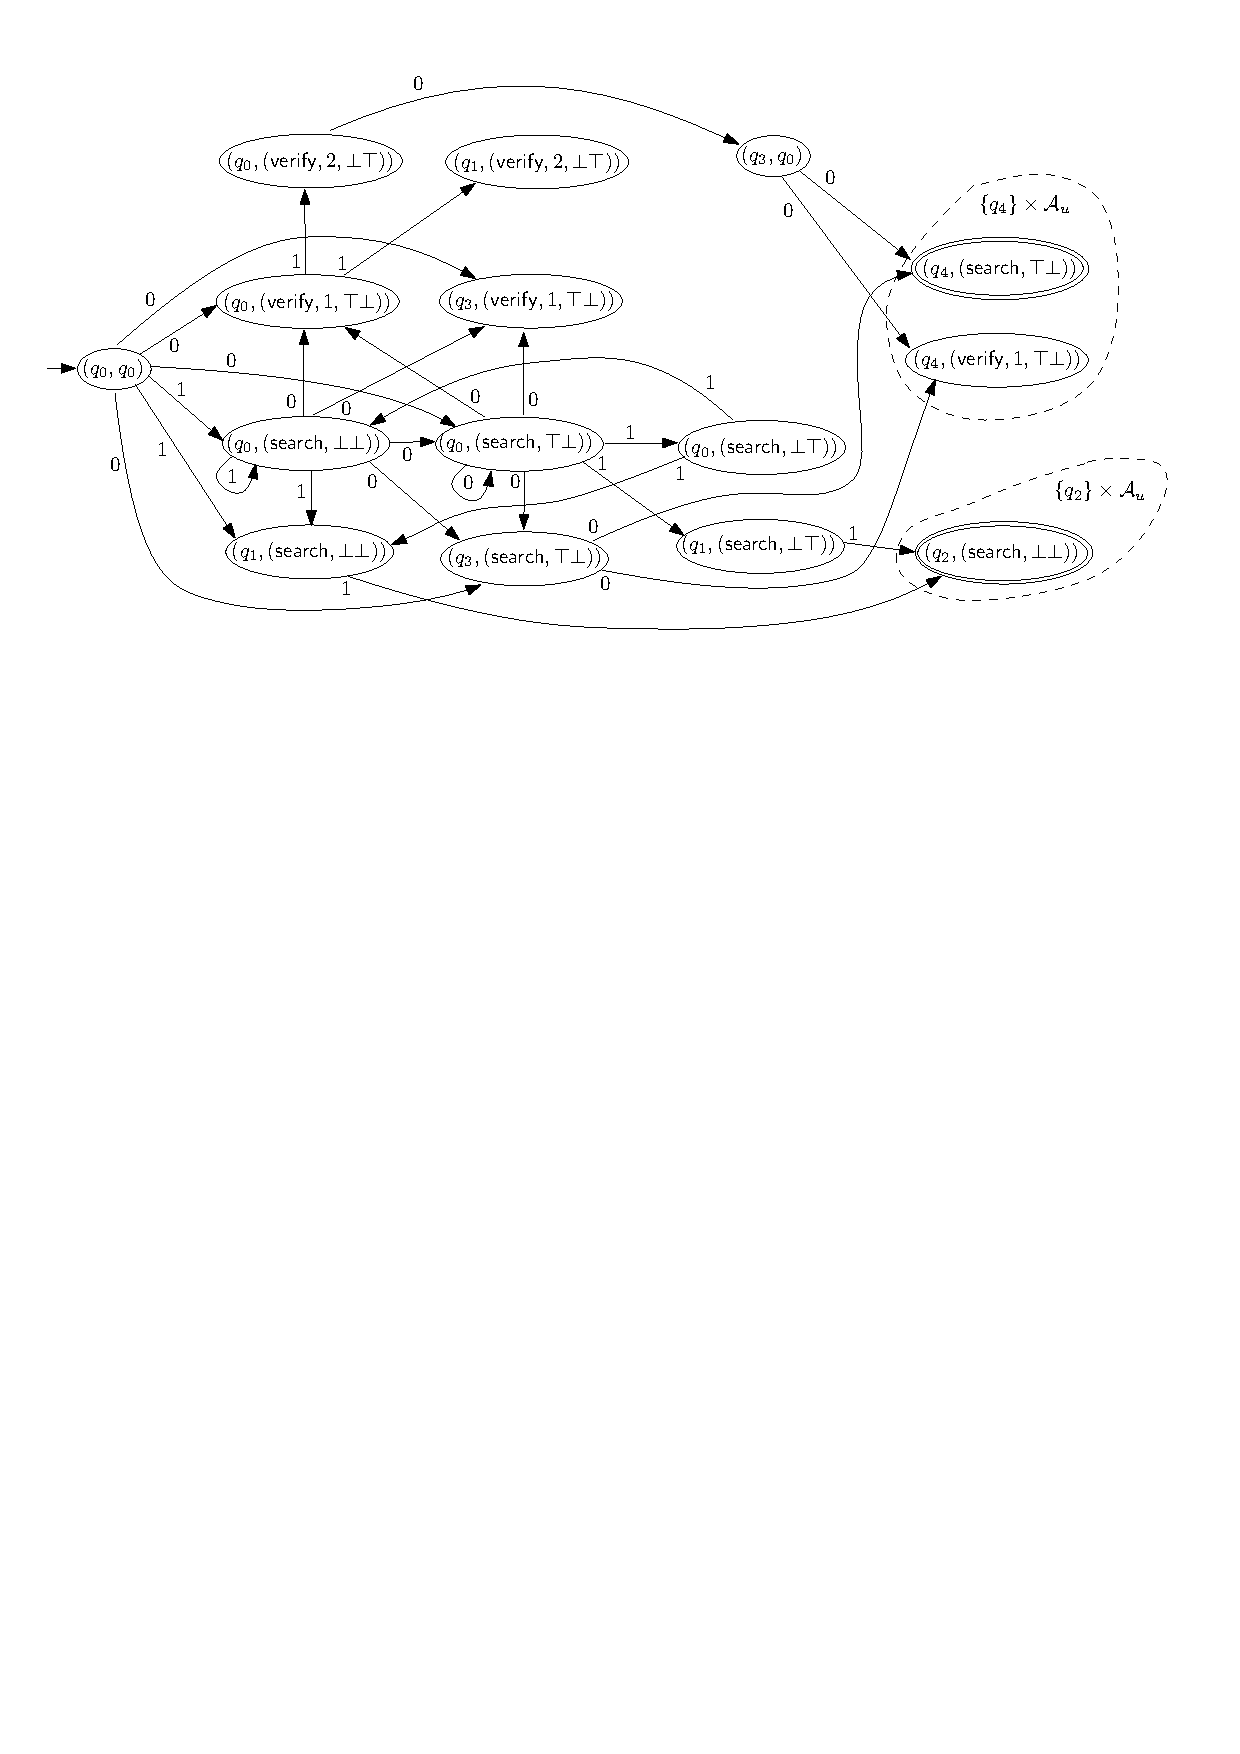
\includegraphics[scale=0.65]{constant-string-example.pdf}
\end{center}
\caption{The NFA $\cA_1 \times \cA_u$ for $u = 010$}\label{fig-cs-exmp}
\end{figure}
%

\def\refsecreplaceallcs{\ref{sec:replaceallcs}}
\section{Complexity analysis in Section~\protect\refsecreplaceallcs}
\label{sec:cs-complexity-full}

We provide a more detailed analysis of the complexity of the algorithm for the constant string case, described in Section~\ref{sec:replaceallcs}.
A summary of this argument already appears in Section~\ref{sec:replaceallcs}.

When constructing $G_{i+1}$ from $G_i$, suppose the two edges from $x$ to $y$ and $z$ respectively are currently removed, let the labels of the two edges be $({\sf l}, u)$ and $({\sf r}, u)$ respectively, then each element $(\cT, \cP)$ of $\cE_i(x)$ may be transformed into an element $(\cT', \cP')$ of $\cE_{i+1}(y)$ such that $|\cT'| = O(|u||\cT|)$, meanwhile, it may also be transformed into an element $(\cT'', \cP'')$ of $\cE_{i+1}(z)$ such that $\cT''$ has the same state space as $\cT$. Thus, for each source variable $x$, $\cE(x)$ contains at most exponentially many elements, and each of them may have a state space of at most exponential size. For instance, for a path from $x'$ to $x$ where the constant strings $u_1,\cdots, u_n$ occur in the labels of edges, an element $(\cT,\cP) \in \cE_0(x')$ may induce an element $(\cT', \cP')$ of $\cE(x)$ such that $|\cT'| \le |\cT| |u_1| \cdots |u_n|$, which is exponential in the worst case. 
%
To solve the nonemptiness problem of the intersection of all these regular constraints, the exponential space is sufficient. Consequently, in this case, we still obtain an EXPSPACE upper bound. 

Let us now consider the special situation that the $\rpleft$-length of $G_C$ is bounded by a constant $c$.
Since $\dmdidx(G_C) \le \lftlen(G_C)$, we know that $\dmdidx(G_C)$ is also bounded by $c$. Therefore, according to Proposition~\ref{prop-di}, there are at most polynomially different paths in $G_C$, we deduce that for each source variable $x$, $\cE(x)$ contains at most polynomially many elements. In addition, since the number of $\rpleft$-edges in each path is bounded by $c$, during the execution of the decision procedure, the number of times when $(\cT, \cP)$ of $\cE_i(x)$ may be transformed into an element $(\cT', \cP')$ of $\cE_{i+1}(y)$ such that $|\cT'| = O(|u||\cT|)$ is bounded by $c$.
Therefore, for each source variable $x$ and each element $(\cT'', \cP'')$ in $\cE(x)$,  $|\cT''|$ is at most polynomial in the size of $C$. We then conclude that for each source variable $x$, $\cE(x)$ corresponds to the intersection of polynomially many regular constraints such that each of them has a state space of polynomial size. Therefore, the nonemptiness of the intersection of all the regular constraints in $\cE(x)$ can be solved in polynomial space. In this situation, we obtain a PSPACE upper bound.


\def\refsecreplaceallre{\ref{sec:replaceallre}}
\section{Complexity analysis in Section~\protect\refsecreplaceallre}
\label{sec:re-complexity-full}

We provide a more detailed analysis of the complexity of the algorithm for the regular-expression case, described in Section~\ref{sec:replaceallre}.
A summary of this argument already appears in Section~\ref{sec:replaceallre}.

In each step of the reduction, suppose the two edges out of $x$ are currently removed, let the two edges be from $x$ to $y$ and $z$ and labeled by $({\sf l}, e)$ and $({\sf r}, e)$ respectively, then each element of $(\cT, \cP)$ of $\cE_i(x)$ may be transformed into an element $(\cT',\cP')$ of $\cE_{i+1}(y)$ such that $|\cT'| = |\cT| \cdot 2^{O(p(|e|))}$, meanwhile, it may also be transformed into an element $(\cT'',\cP'')$ of $\cE_{i+1}(y)$ such that $\cT''$ has the same state space as $\cT$. Thus, after the reduction, for each source variable $x$, $\cE(x)$ may contain exponentially many elements, and each of them may have a state space of exponential size, more precisely, if we start from a vertex $x$ without predecessors, with an element $(\cT,\cP)$ in $\cE_0(x)$, and go to a source variable $y$ through a path where $k$ edges have been traversed and removed, let $e_1,\cdots, e_k$ be the regular expressions occurring in the labels of these edges, then the resulting element in $\cE(y)$ has a state space of size $|\cT| \cdot 2^{O(p(|e_1|))} \cdot 2^{O(p(|e_2|))} \cdot \cdots \cdot 2^{O(p(|e_k|))}$ in the worst case. To solve the nonemptiness problem of the intersection of all these regular constraints, the exponential space is sufficient. Consequently, for the most general case of regular expressions, we still obtain a EXPSPACE upper bound. 

On the other hand, for the situation that the $\rpleft$-length of $G_C$ is at most one, we wan to show that the algorithm runs in polynomial space. Suppose the $\rpleft$-length of $G_C$ is at most one. Then the diamond index of $G_C$ is at most one as well. According to Proposition~\ref{prop-di}, there are only polynomially many paths in $G_C$. Nevertheless, for each source variable $x$, $\cE(x)$ may contain an element $(\cT,\cP)$ such that $|\cT|$ is exponential. Since $|\cP|$ may be exponential, $(\cT,\cP)$ may correspond to the intersection of exponentially many regular constraints. However, we can show that $|\cP|$ is at most polynomial, as a result of the fact that the $\rpleft$-length of $G_C$ is at most one. The arguments proceed as follows: Suppose two edges from $x$ to $y, z$ respectively are removed, and an element $(\cT', \cP')$ of $\cE_{i+1}(y)$ such that $|\cT'|$ is exponential and $|\cP'|$ is polynomial, is generated from an element of $(\cT, \cP)$ of $\cE_i(x)$. Then $y$ must be a source variable in $G_C$. Otherwise, there is an $\rpleft$-edge out of $y$ and the $\rpleft$-length of $G_C$ is at least two, a contradiction. Therefore, $y$ is a source variable in $G_C$, $(\cT', \cP')$  will not be used to generate the regular constraints for the other variables. In other words, $y$ is a source variable in $G_C$, and $(\cT', \cP') \in \cE(y)$ with $|\cP'|$ polynomial. We then conclude that for each source variable $x$, $|\cE(x)|$  is at most polynomial in the size of $C$ and for each element $(\cT, \cP) \in \cE(x)$, $|\cP|$ is polynomial in the size of $C$. Therefore, for each source variable $x$,  $\cE(x)$ corresponds to the intersection of polynomially many regular constraints, where each of them has a state space at most exponential size. To solve the nonemptiness of the intersection of these regular constraints, the polynomial space is sufficient. We obtain a PSPACE upper bound for the situation that the $\rpleft$-length of $G_C$ is at most one.


\def\refsecext{\ref{sec-ext}}
\section{Undecidability Proofs for Section~\protect\refsecext}
\label{sec:ext-undec-proofs}

\subsection{Proof of Theorem~\ref{thm-ext-int}}

\begin{proof}
	The basic idea of the reduction is to simulate the two polynomials $f(x_1,\cdots, x_n)$ and $g(x_1,\cdots, x_n)$, where $x_1,\cdots,x_n$ range over the set of natural numbers, with two $\strline[\concat,\replaceall]$ formulae $C_f, C_g$ over a unary alphabet $\{a\}$, with the output string variables $y_f, y_g$ respectively, and simulate the equality $f(x_1,\cdots, x_n) = g(x_1,\cdots, x_n)$ with the integer constraint $|y_f|=|y_g|$ (which is equivalent to $y_f = y_g$, since $y_f, y_g$ represent strings over the unary alphabet $\{a\}$). 
	
	A polynomial $f(x_1,\cdots, x_n)$ or $g(x_1,\cdots, x_n)$ where $x_1, \cdots, x_n$ range over the set of natural numbers, can be simulated by an $\strline[\concat,\replaceall]$ formula over an unary alphabet $\{a\}$ as follows: The natural numbers are represented by the strings over the alphabet $\{a\}$. A string variable is introduced for each subexpression of $f(x_1,\cdots, x_n)$. The numerical addition operator $+$ is simulated by the string operation $\concat$ 
	%\mat{$\concat$ is not part of $\strline[\replaceall]$, can it be simulated when the string alphabet is unary, or do we need two extra characters?}\zhilin{changed to $\strline[\concat,\replaceall]$.}
	and the multiplication operator $*$ is simulated by $\replaceall$. Since it is easy to figure out how the simulation proceeds, we will only use an example to illustrate it and omit the details here. Let us consider $f(x_1,x_2) = x_1^2 + 2 x_1 x_2 + 5$. By abusing the notation, we also use $x_1,x_2$ as string variables in the simulation. We will introduce a string variable for each subexpression in $f(x_1,x_2)$, namely the variables $y_{x_1^2}, y_{x_1x_2}, y_{2x_1x_2}, y_{x_1^2+2x_1x_2}, y_{f(x_1,x_2)}$. Then $f(x_1,x_2)$ is simulated by the $\strline[\concat,\replaceall]$ formula
	\[
	\begin{array} {l c l }
	C_f & \equiv & y_{x_1^2} = \replaceall(x_1,a, x_1)\ \wedge y_{x_1x_2} = \replaceall(x_1, a, x_2)\ \wedge \\
	& & y_{2x_1x_2} = \replaceall(aa, a, y_{x_1x_2})\ \wedge y_{x_1^2+2x_1x_2} = y_{x_1^2} \concat y_{2x_1x_2}\ \wedge  \\
	& & y_{f(x_1,x_2)}=y_{x_1^2+2x_1x_2} \concat a a a a a\ \wedge x_1 \in a^*\ \wedge x_2 \in a^*.
	\end{array}
	\]
	Then according to Proposition~\ref{prop-concat}, $C_f, C_g$ can be turned into equivalent $\strline[\replaceall]$ formula $C'_f, C'_g$ by introducing fresh letters.
	%\mat{But we may have to give up the unary alphabet?}\zhilin{yes, you are  right, it is fine.}
	
	Since $C'_f$ and $C'_g$ share only source variables $x_1,\cdots, x_n$, we know that $C'_f \wedge C'_g$ is still an $\strline[\replaceall]$ formula.
	From the construction of $C'_f, C'_g$, it is evident that for every pair of polynomials $f(x_1,\cdots, x_n)$ and $g(x_1,\cdots, x_n)$, $f(x_1,\cdots, x_n) = g(x_1,\cdots, x_n)$ has a solution in natural numbers iff $C'_f \wedge C'_g \wedge |y_f| = |y_g|$ is satisfiable. The proof is complete.
	%
	%%%%%%%%%%%%%%%%%%%%%%%%%%%%%%%%%%%%%%%%%%%%%%%%%%%%%%%%%%%
	%%%%%%%%%%%%%%%%%%%%%%%%%%%%%%%%%%%%%%%%%%%%%%%%%%%%%%%%%%%
	\hide{
		We shall reduce from the aforementioned version of the Hilbert tenth problem. For any polynomial with positive integral  $f(x_1, \cdots, x_n)$ where each coefficient is a positive, we can construct a (division-free) arithmetic circuit (AC) is a directed  acyclic graph with nodes labelled with constants from $\mathbb{Z}$, or with some indeterminates $X_1, \cdots, X_m$, or with the operators $+, -, *$. The nodes labelled with constants are called constant nodes, while those labelled with indeterminates are called input nodes. Both constant and input nodes do not have incoming edges. Internal nodes are those labelled with $+,-,*$. Output node is the one which does not have out-going edges. Without loss of generality we assume that each internal node has in-degree 2, and there is only one output node. Each node in the circuit represents a multivariate polynomial $\mathbb{Z}[X_1, \cdots, X_m]$. Vice verse, each polynomial $f\in \mathbb{Z}[X_1, \cdots, X_m]$ can be represented as an AC, and, if the polynomial has only positive (integral) coefficients, the corresponding AC does not contain nodes labelled by $-$ or negative constants.  
		
		We observe that, given an AC, one can construct an SL[$\concat, \replaceall$] formula over the alphabet $\Sigma=\{a\}$ as follows. Each node $n$ of the AC is associated with a string variable $x_n$. As a result, each input node of the AC labelled by $X_i$ (i.e., the indeterminate) corresponds to a  source variable.   
		\begin{itemize}
			\item For each internal node $n$ labelled by $+$, suppose that $n$ has two children nodes $n_l$ and $n_r$, we introduce a string constraint $x_n= x_{n_l}\concat x_{n_l}$.  
			
			\item For each internal node $n$ labelled by $*$, suppose that $n$ has two children nodes $n_l$ and $n_r$, we introduce a string constraint $x_n= \replaceall(x_{n_l}, a, x_{n_l})$.  		
		\end{itemize}
		Furthermore, we introduce, for each node $n$ labelled by a constant $c$, a regular constraint $x_n=a^c$. 
		
		It is straightforward to verify, according to the semantics of SL[$\concat, \replaceall$], that:
		\begin{itemize}
			\item for relational constraint $x_n= x_{n_l}\concat x_{n_l}$, $|x_n|= |x_{n_l}|+|x_{n_l}|$; 
			\item for relational constraint $x_n= \replaceall(x_{n_l}, a, x_{n_l})$,  $|x_n|= |x_{n_l}|\cdot |x_{n_l}|$; and 
			\item for regular $x_n=a^c$, $|x_n|=c$. 
		\end{itemize}
		
		It follows that for each polynomial $f(x_1, \cdots, x_m)$ with positive integral coefficients, we can construct a straight-line string constraint $\varphi_{f}\wedge\psi_g$ over $\Sigma=\{a\}$ with $y_f$ as the output variant and $y_1, \cdots, y_n$ as source variables such that
		$f(c_1, \cdots, c_m)=|y|$ and, for each $1\leq i\leq m$, $|y_i|= c_i$ (i.e., $y_i=a^{c_i}$).  
		
		Consequently, when given two polynomials $f(x_1, \cdots, x_m)$ and $g(x_1, \cdots, x_m)$, we have straight-line string constraints $\varphi_{f}\wedge \varphi_{g}\wedge \psi_{f}\wedge \psi_g$ with two distinguished two variables  $y_f$ and $y_g$ such that  
		\[\exists x_1, \cdots, x_m. f(x_1, \cdots, x_m)=g(x_1, \cdots, x_m)\mbox{ iff } |y_f|=|y_g|\wedge \varphi_{f}\wedge \varphi_{g}\wedge \psi_{f}\wedge \psi_g\mbox{ is satisfiable} \]
		
		Finally, note that any  SL[$\concat, \replaceall$] constraints can be transformed into SL[$\replaceall$] constraints, we obtain a reduction from the Hilbert's 10th problem to the satisfiability problem of  SL[$\replaceall$] with length constraints, which entail that the latter problem is undecidable. The proof is completed. 
	}
	%%%%%%%%%%%%%%%%%%%%%%%%%%%%%%%%%%%%%%%%%%%%%%%%%%%%%%%%%%%
	%%%%%%%%%%%%%%%%%%%%%%%%%%%%%%%%%%%%%%%%%%%%%%%%%%%%%%%%%%%
\end{proof}

\subsection{Undecidability of Depth-1 dependency graph}

A \emph{linear polynomial} (resp.\ quadratic polynomial) is a polynomial with degree at most one (resp.\ with degree at most two) where each coefficient is an integer. %of the form $a_0 + a_1x_1 + \cdots + a_n x_n$ (resp. a polynomial with degree at most two) where each coefficient $a_i\in \mathbb{Z}$  for $0 \leq i \leq n$. A quadratic polynomial

\begin{theorem}[\cite{ID04}]\label{thm-quad-eq}
	%	There exists some (fixed) $k$ such that no algorithm can solve Diophantine systems in the following form
	%	\[y_1F_1=G_1, t_1H_1=I_1, \cdots, t_kF_k = G_k, t_kH_k = I_k,\] 
	%
	%	where $F_i, G_i, H_i, I_i$ for $1\leq i\leq k$ are nonnegative linear polynomials over natural number variables  $s_1, \cdots, s_m$.
	The following problem is undecidable: Determine whether a system of equations of the following form has a solution in natural numbers, 
	\[
	\begin{array} {l l }
	A_i = B_i, & i =1, \cdots, k,\\
	y_iF_i=G_i \wedge y_i H_i = I_i, & i =1, \cdots, m, 
	\end{array}
	\] 
	%
	where $A_i, B_i, F_i, G_i$ are linear polynomials on the variables $x_1,\cdots, x_n$ (Note that each variable $y_i$ occurs in exactly two quadratic equations).
\end{theorem}

We can get a reduction from the problem in Theorem~\ref{thm-quad-eq} to the satisfiability of the extension of $\strline[\replaceall]$ with integer constraints as follows: For each monomial $y_i x_j$ in the quadratic polynomials, we use an $\strline[\replaceall]$ formula $z_{y_i x_j} = \replaceall(y_i, a, x_j)$ to simulate $y_i x_j$, where $z_{y_i x_j}$ are freshly introduced string variables. Since each equation $y_iF_i=G_i$ or $y_i H_i = I_i$ can be seen as a linear combination of the terms $y_i x_j$ and $x_j$ for $i \in [m]$ and $j \in [n]$, we can replace each variable $x_j$ with $|x_j|$, and each term $y_ix_j$ with $|z_{y_i x_j}|$,  thus transform them into the (linear) integer constraints $F'_i = G'_i$ or $H'_i = I'_i$. Similarly, after replacing each variable $x_j$ with $|x_j|$, we transform each equation $A_i= B_i$ into an integer constraint $A'_i = B'_i$. Therefore, we get a formula 
$$
\begin{array}{l c l }
\bigwedge \limits_{i \in [m], j \in [n]} z_{y_i x_j} = \replaceall(y_i, a, x_j) \wedge \bigwedge \limits_{i \in [m]} y_i \in a^*\ \wedge  \bigwedge \limits_{j \in [n]} x_j \in a^* \  \wedge\\
\hspace{2cm} \bigwedge \limits_{i \in [k]} A'_i = B'_i \wedge \bigwedge \limits_{i \in [m]} (F'_i = G'_i \wedge H'_i = I'_i),
\end{array}
$$
where the dependency graph of the $\strline[\replaceall]$ subformula is of depth at most one.

%%%%%%%%%%%%%%%%%%%%%%%%%%%%%%%%%%%%%%%%%%%%%%%%%
%%%%%%%%%%%%%%%%%%%%%%%%%%%%%%%%%%%%%%%%%%%%%%%%%
\hide{
	From this class of quadratic Diophantine equations, we can introduce string variables $x_1, \cdots, x_k$ and $y_1, \cdots, y_m$, together with relational string constraints 
	\[z_{i,j}=\replaceall(x_i, a, y_j)\]
	for $1\leq i\leq k$ and $1\leq j\leq m$. Note that, for each $i$,  $t_i F_i=G_i$ can be written as
	\begin{equation} \label{eq:dio}
	t_i\cdot \left(a_0+\sum_{j=1}^s a_j s_j\right) =  b_0+\sum_{j=1}^s b_j s_j
	\end{equation}
	where $a$'s and $b$'s are all natural numbers. Moreover, \eqref{eq:dio} holds iff 
	\[a_0\cdot |y_i|+ \sum_{j=1}^s a_j |z_{i,j}| =  b_0+ \sum_{j=1}^s b_j |x_j| \] 
	which is an integer constraint defined in Definition~\ref{def:intconst}. This entails that
}
%%%%%%%%%%%%%%%%%%%%%%%%%%%%%%%%%%%%%%%%%%%%%%%%%
%%%%%%%%%%%%%%%%%%%%%%%%%%%%%%%%%%%%%%%%%%%%%%%%%

\subsection{Undecidability of the character constraints}

\begin{proposition}\label{prop-ext-char}
	For the extension of $\strline[\replaceall]$ with character constraints, the satisfiability problem is undecidable. 
\end{proposition}

The arguments for Proposition~\ref{prop-ext-char} proceed as follows. Recall that in the proof of Theorem~\ref{thm-ext-int}, we get a formula $C_f \wedge C_g \wedge |y_f| = |y_g|$ such that $f(x_1,\cdots, x_n) = g(x_1,\cdots, x_n)$ has a solution in natural numbers iff $C_f \wedge C_g \wedge |y_f| = |y_g|$ is satisfiable. Let $\$ \neq a$. Suppose  $z_f = y_f \concat \$$, and $z_g = y_g \concat \$$. Then $|y_f| = |y_g|$ can be captured by $z_f[\mathfrak{n}] = \$[1] \wedge  z_g[\mathfrak{n}] = \$[1]$, where $\mathfrak{n}$ is a variable of type $\intnum$. More precisely, 
%
we have 
\begin{quote}
	\centering
	$C_f \wedge C_g \wedge |y_f|= |y_g|$ is satisfiable \\
	%
	iff \\
	%
	$C_f \wedge C_g \wedge z_f = y_f \concat \$ \wedge z_g = y_g \concat \$ \wedge z_f[\mathfrak{n}] = \$[1] \wedge  z_g[\mathfrak{n}] = \$[1]$ is satisfiable. 
\end{quote}
Therefore, we get a reduction from Hilbert's tenth problem to the satisfiability problem for the extension of $\strline[\replaceall]$ with character constraints. 

%For any two string variables $x,y$ on the unary alphabet $\{a\}$, let $x' = x \concat \$$ and $y' = y \concat \$$, then $|x| = |y|$ iff .
%
% $|x|=|y|$ iff $\exists n. x[n]=y[n]=\$$. 
%
%
%\begin{lemma}
%	For any two strings $x,y\in a^*\$$, $|x|=|y|$ iff $\exists n. x[n]=y[n]=\$$. 
%\end{lemma}
%
%As SL[$\replaceall$] with length constraints is undecidable, we conclude that 
%
%
%
%\tl{I am not satisfied with this as the quantifier is used}

\subsection{Undecidability of the $\indexof$ constraints}

\begin{proposition}\label{prop-indexof}
	For the extension of $\strline[\replaceall]$ with the $\indexof$ constraints, the satisfiability problem is undecidable. 
\end{proposition}

Proposition~\ref{prop-ext-char} follows from the following observation and Theorem~\ref{thm-ext-int}: For any two string variables $x,y$ over a unary alphabet, 
$1= \indexof(x,y)$ iff $x$ is a prefix of $y$. Therefore, $|x| = |y|$ iff $1=  \indexof(x,y) \wedge 1= \indexof(y,x)$. This implies that in the proof of Theorem~\ref{thm-ext-int}, we can replace $|y_f| = |y_g|$ with $1=\indexof(y_f, y_g) \wedge 1 = \indexof(y_g, y_f)$ and get a reduction from Hilbert's tenth problem to the satisfiability problem for the extension of $\strline[\replaceall]$ with the $\indexof$ constraints.
Note that $=$ can be simulated as a conjunction of $\leq$ and $\geq$.


%We have the following observation: 
%\begin{lemma}
%	For any two strings $x,y$ over $\{a\}$, $x=y$ iff $1=\indexof(x,y)=\indexof(y,x)$.  
%\end{lemma}
%
%It follows that 

%\subsection*{Further undecidability results}


\def\refsecreplaceallre{\ref{sec:replaceallre}}
\section{Examples in Section~\protect\refsecreplaceallre}

\begin{example}\label{exmp-pa-re}
	Let $e_0 = 0^*0 1(1^* + 0^*)$. Then $\cA_{0}$ and $\cA_{e_0}$ are illustrated in Figure~\ref{fig-pa-re}, where ${\sf sleft}$ and ${\sf slong}$ are the abbreviations of $\searchleft$ and $\searchlong$ respectively. Let us use the state $(\{q_{0,1}\}\{q_{0,0}\}, {\sf sleft}, \emptyset)$ to illustrate the construction. Since $\big(\delta_0(\{q_{0,1}\}, 0) \cup \delta_0(\{q_{0,0}\}, 0)\big) \cap F_0 = \{q_{0,1}\} \cap F_0 = \emptyset$, $\delta_0(\emptyset, 0) \cap F_0 = \emptyset$, and $\red(\delta_0(\{q_{0,1}\}, 0) \delta_0(\{q_{0,0}\}, 0))=\{q_{0,1}\}$, we deduce that the transition $((\{q_{0,1}\}\{q_{0,0}\}, {\sf sleft}, \emptyset), 0, (\{q_{0,1}\} \{q_{0,0}\}, {\sf sleft}, \emptyset)) \in \delta_{e_0}$. On the other hand, it is impossible to go from the state $(\{q_{0,1}\}\{q_{0,0}\}, {\sf sleft}, \emptyset)$ to the ``$\searchlong$'' mode. This is due to the fact that $\delta_0(\{q_{0,0}\}, 0)=\{q_{0,1}\} \subseteq \delta_0(\{q_{0,1}\},0)=\{q_{0,1}\}$. In addition, there are no $1$-transitions out of $(\{q_{0,1}\}\{q_{0,0}\}, {\sf sleft}, \emptyset)$. This is due to the fact that $\delta_0(\{q_{0,1}\}, 1) \cap F_0 = \{q_{0,2}, q_{0,3}\} \cap F_0 \neq \emptyset$.
	%
	\begin{figure}[htbp]
		\begin{center}
			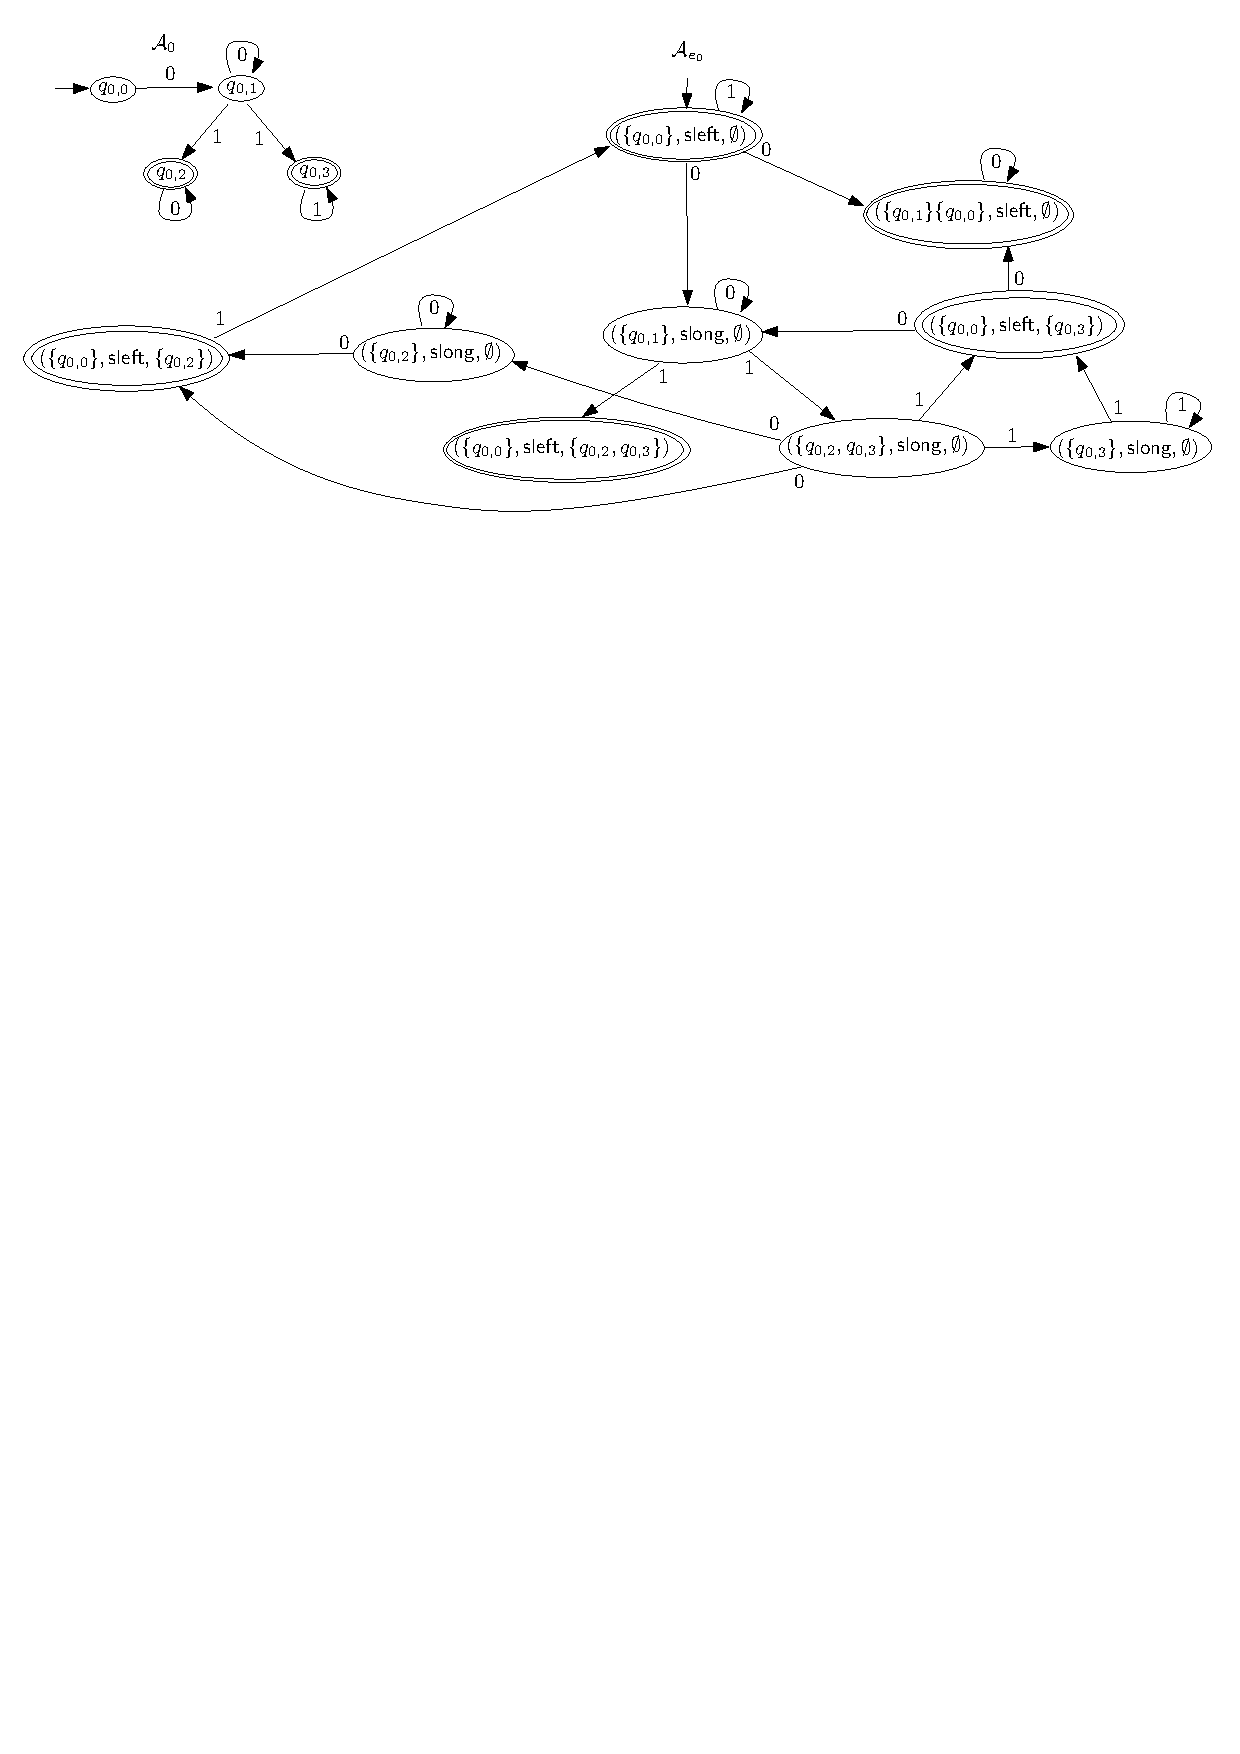
\includegraphics[scale=0.7]{regular-expression-example.pdf}
		\end{center}
		\caption{The NFA $\cA_0$ and $\cA_{e_0}$ for $e_0 = 0^*0 1(1^* + 0^*)$}\label{fig-pa-re}
	\end{figure} 
\end{example}

\begin{example}
	Let $C \equiv x = \replaceall(y, e_0, z) \wedge x \in e_1 \wedge y \in e_2 \wedge z \in e_3$, where $e_1,e_2,e_3$ are as in Example~\ref{exmp-sl} (cf. Figure~\ref{fig-sl-exmp}) and $e_0$ is as in Example~\ref{exmp-pa-re} (cf. Figure~\ref{fig-pa-re}). Suppose $T_z = \{(q_0, q_0), (q_1, q_2)\}$. Then the NFA $\cB_{\cA_1, e_0, T_z}$ is as illustrated in Figure~\ref{fig-re-exmp}, where the thick edges denote the added transitions. Let us use the state $(q_1, (\{q_{0,0}\}, \searchleft, \emptyset))$ to exemplify the construction. The transition $((q_1, (\{q_{0,0}\}, \searchleft, \emptyset)), 1, (q_2, (\{q_{0,0}\}, \searchleft, \emptyset)))$ is  in $\cA_1 \times \cA_{e_0}$. Since $\delta_0(q_{0,0}, 1) \cap F_0 = \emptyset$, this transition is not removed and is thus in $\cB_{\cA_1, e_0, T_z}$. On the other hand, since there are no $0$-transitions out of $q_1$ in $\cA_1$, there are no $0$-transitions from $(q_1, (\{q_{0,0}\}, \searchleft, \emptyset))$ to some state from $Q_{\searchleft}$ in $\cB_{\cA_1, e_0, T_z}$. 
	Moreover, because $((\{q_{0,0}\}, \searchleft, \emptyset), 0, (\{q_{0,1}\}, \searchlong, \emptyset)) \in \delta_{e_0}$ and $(q_1, q_2) \in T_z$, the transition $((q_1, (\{q_{0,0}\}, \searchleft, \emptyset)), 0, (q_1, (\{q_{0,1}\}, \searchlong, \emptyset)))$ is added. 
	One may also note that there are no 0-transitions from $(q_2, (\{q_{0,0}\}, \searchleft, \emptyset))$ to the state $(q_2, (\{q_{0,1}\}, \searchlong, \emptyset))$, because there are no pairs $(q2,-) \in T_z$.
	It is not hard to see that $010101 \in \Ll(\cA_2) \cap \Ll(\cB_{\cA_1, e_0, T_z})$. In addition, $10 \in \Ll(\cA_3) \cap \Ll(\cA_1(q_0,q_0)) \cap \Ll(\cA_1(q_1,q_2))$. Let $y$ be $010101$ and $z$ be $10$. Then $x$ takes the value $\replaceall(010101, e_0, 10)=10 \cdot \replaceall(101, e_0, 10)=10110$, which is accepted by $\cA_1$. Therefore, $C$ is satisfiable.
	\begin{figure}[htbp]
		\begin{center}
			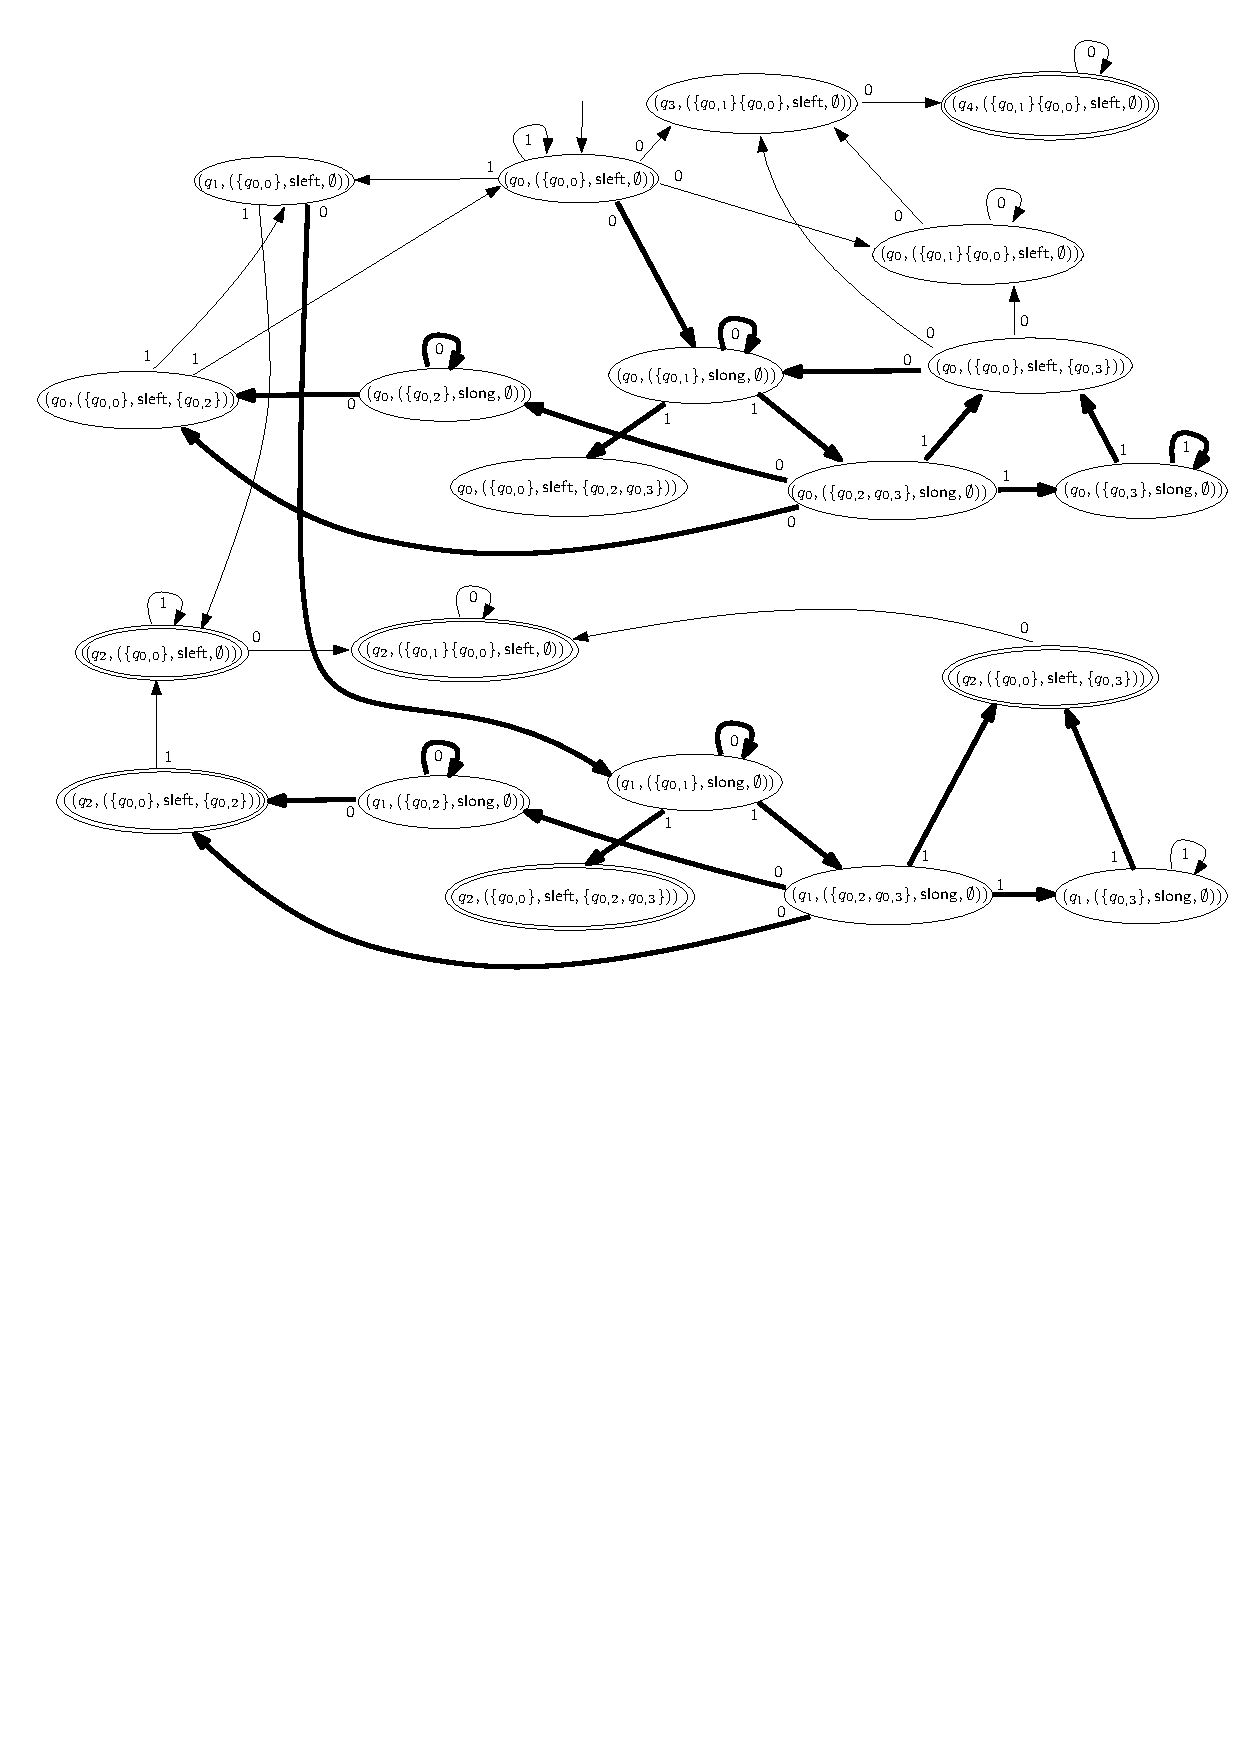
\includegraphics[scale=0.68]{regular-expression-example-2.pdf}
		\end{center}
		\caption{The NFA $\cB_{\cA_1, e_0, T_z}$}\label{fig-re-exmp}
	\end{figure} 
\end{example}


\end{appendix}

%\fi

\end{document}
